\documentclass[11pt]{article}
\usepackage[margin=1in]{geometry}
\usepackage[T1]{fontenc}
\usepackage[utf8]{inputenc}
\usepackage{amsmath, amssymb, amsfonts}
\usepackage{graphicx}
\usepackage{booktabs}
\usepackage{float}
\usepackage{hyperref}
\title{Scientific Analysis of Moral Judgments using Tobit and Cluster-Aware Non-Parametric Robustness Models}
\author{Automated Research Pipeline}
\date{marzo 28, 2026}
\begin{document}
\maketitle

\section{Dataset and Sample Description}
The empirical foundation of this project rests on two primary experimental datasets: FLORIDA and BUC.  The sample consists of students from the Bucaramanga Campus.  These datasets capture incentivized moral judgments from distinct socio-economic contexts. Participants were presented  with standardized negotiation scenarios where a negotiator's decision resulted in varying degrees of payoff for  themselves, their own group, and a victim group. Under  Option 2: explicit case-configuration modeling , each judgment is treated as relational and indexed by an explicit victim x negotiator scenario configuration rather than by isolated ingroup/outgroup attributes.

\section{Datacard and Variable Definitions}
The following table defines the primary symbols and variables used in the mathematical specifications and hypothesis tests.
\begin{table}[H]
\centering
\caption{Symbols and Variable Dictionary.}
\label{tab:symbols}
\resizebox{\textwidth}{!}{%
\begin{tabular}{ll}
\toprule
Symbol & Definition \\
\midrule
$y_{ij}$ & Observed moral judgment of scenario $j$ by participant $i$. \\
$y^*_{ij}$ & Latent moral preference score (unbounded). \\
$\beta_1$ & Regression coefficient representing the marginal effect of the predictor. \\
$\beta_{0.5}$ & Median-regression coefficient from the non-parametric censored robustness model. \\
$Q_{0.5}(y^*_{ij} \mid \mathbf{x}_{ij})$ & Conditional median of the latent bounded outcome given the predictors. \\
$\text{IRI}_i$ & Empathy score (Average composite of the Interpersonal Reactivity Index). \\
$\text{CaseConfig}_{ij}$ & Explicit victim x negotiator case-configuration factor capturing relational scenarios such as \texttt{Hum\_x\_Hum}, \texttt{Hum\_x\_Ing}, \texttt{Hum\_x\_Control}, \texttt{Ing\_x\_Hum}, \texttt{Ing\_x\_Ing}, \texttt{Ing\_x\_Control} . \\
$\text{Role}_{ij}$ & Scenario-role conditioning indicator distinguishing Observer from Victim judgments. \\
$\text{Decision}_{ij}$ & Decision-context conditioning indicator distinguishing Accept from Reject judgments. \\
$\text{ICC}$ & Intraclass Correlation: ratio of between-cluster variance to total variance. \\
\bottomrule
\end{tabular}
}
\end{table}
Option 2: explicit case-configuration modeling frames each judgment as a relational victim x negotiator case. The paired-group structure generates interpretable configurations such as Hum\_x\_Hum, Hum\_x\_Ing, Hum\_x\_Control, Ing\_x\_Hum, Ing\_x\_Ing, and Ing\_x\_Control, with role (Observer/Victim) and decision context (Accept/Reject) available as further conditioning dimensions.

\section{Hypotheses to Test}
\begin{itemize}
  \item \textbf{H1 (Empathy):} Higher empathy predicts lower moral-judgment scores for harmful decisions after conditioning on explicit victim x negotiator case configurations.
  \item \textbf{H2a (Relational Betrayal):} Same-faculty and cross-faculty betrayal cases are evaluated through explicit victim x negotiator configurations rather than a single same-group indicator.
  \item \textbf{H2b (Case Configuration):} Relational judgments are interpreted through explicit case contrasts such as \texttt{Hum\_x\_Hum}, \texttt{Hum\_x\_Ing}, \texttt{Hum\_x\_Control}, \texttt{Ing\_x\_Hum}, \texttt{Ing\_x\_Ing}, \texttt{Ing\_x\_Control}.
  \item \textbf{H3 (Moderation):} The empathy effect may vary across explicit victim x negotiator case configurations.
\end{itemize}

\section{Mathematical Approach and Theoretical Foundations}
The analysis employs two complementary estimators for bounded moral judgments. The primary specification is a Two-Limit Tobit model, which is theoretically appropriate for dependent variables that are 
strictly bounded within a known interval. In this context, moral judgments ($y_{ij}$) are observed on a scale from -9 to 9. 
The Tobit model assumes the existence of a latent, unobserved preference index ($y^*_{ij}$) that follows a linear relationship. 
Option 2 replaces isolated ingroup/outgroup indicators with explicit relational case configurations built from the paired-group structure of each judgment. The current project records the victim group first and the judged negotiator label second, so configurations such as \texttt{Hum\_x\_Hum}, \texttt{Hum\_x\_Ing}, \texttt{Hum\_x\_Control}, \texttt{Ing\_x\_Hum}, \texttt{Ing\_x\_Ing}, \texttt{Ing\_x\_Control} refer to victim x negotiator combinations rather than detached attributes.
 The core design vector therefore includes empathy, explicit case-configuration contrasts, and contextual conditioning terms such as role and decision context:

$$y^*_{ij} = \beta_0 + \beta_1 \text{IRI}_i + \boldsymbol{\gamma}'\text{CaseConfig}_{ij} + \boldsymbol{\delta}'\text{Context}_{ij} + \epsilon_{ij}, \quad \epsilon_{ij} \sim N(0, \sigma^2)$$

The actual observed judgment $y_{ij}$ relates to this latent variable via the censoring transformation:

$$y_{ij} = \max(-9, \min(9, y^*_{ij}))$$

This approach prevents the 'ceiling' and 'floor' effects from biasing the linear coefficients, as would occur in standard OLS regression.

Because the Tobit model relies on a Gaussian latent-error assumption, the pipeline also fits a distribution-robust censored median specification implemented as interval-censored quantile regression ($p = 0.5$). 
This complementary estimator targets the conditional median of the latent bounded outcome and is less sensitive to heavy tails and non-normal disturbances:

$$Q_{0.5}(y^*_{ij} \mid \mathbf{x}_{ij}) = \mathbf{x}_{ij}'\beta_{0.5}$$

The non-parametric branch preserves the censoring structure while relaxing the parametric normality assumption. The Tobit and robustness results should therefore be interpreted jointly: Tobit provides the clustered parametric benchmark with participant-clustered standard errors by id, while the non-parametric branch first establishes a converged full-sample censored median fit and then, in the default pipeline, adds participant-level cluster bootstrap inference that resamples ids with replacement and retains all repeated observations from each sampled participant. In both branches, id is used only to account for within-participant dependence and is not a substantive explanatory variable.

\section{Analysis of Sample Size Impact}
The statistical validity of our inferences depends on the trade-off between False Positives (Type I error, $\alpha$) 
and False Negatives (Type II error, $\beta$). Given the clustered nature of our data, sample size impact is not 
merely a count of observations, but a function of cluster correlation.

\subsubsection{Step-by-Step Sensitivity Analysis}
To determine the impact of our sample size on our ability to detect effects, we follow these steps:

1. Calculate the Design Effect (Deff): As multiple judgments are nested within individuals, we adjust for the Intraclass Correlation (ICC).
$$Deff = 1 + (m - 1) \times ICC$$
where $m$ is the average number of scenarios per participant. 

2. Determine the Effective Sample Size (ESS): The ESS represents the number of independent observations that would provide the same statistical power as our clustered sample.
$$ESS = \frac{n_{total}}{Deff}$$

3. Inference Impact: A higher ICC reduces the ESS, thereby increasing the Standard Error of our Tobit coefficients. 
If the ESS is low, our models become 'conservative', increasing the risk of Type II errors (failing to support a hypothesis). 
By using clustered robust standard errors for Tobit and participant-level cluster bootstrap inference for the non-parametric robustness model after each converged full-sample fit, we ensure that both sets of p-values acknowledge this reduced information density, 
protecting the integrity of our Type I error threshold ($\alpha = 0.05$).

Based on the current run, the observed Intraclass Correlation (ICC) is 0.717, with an Effective Sample Size (ESS) of 266.9.

\section{Descriptive Statistics}
The empathy profile of the sample is visualized in Figure \ref{fig:radar}, showing the average scores across the four IRI latent variables.
\begin{figure}[H]
\centering
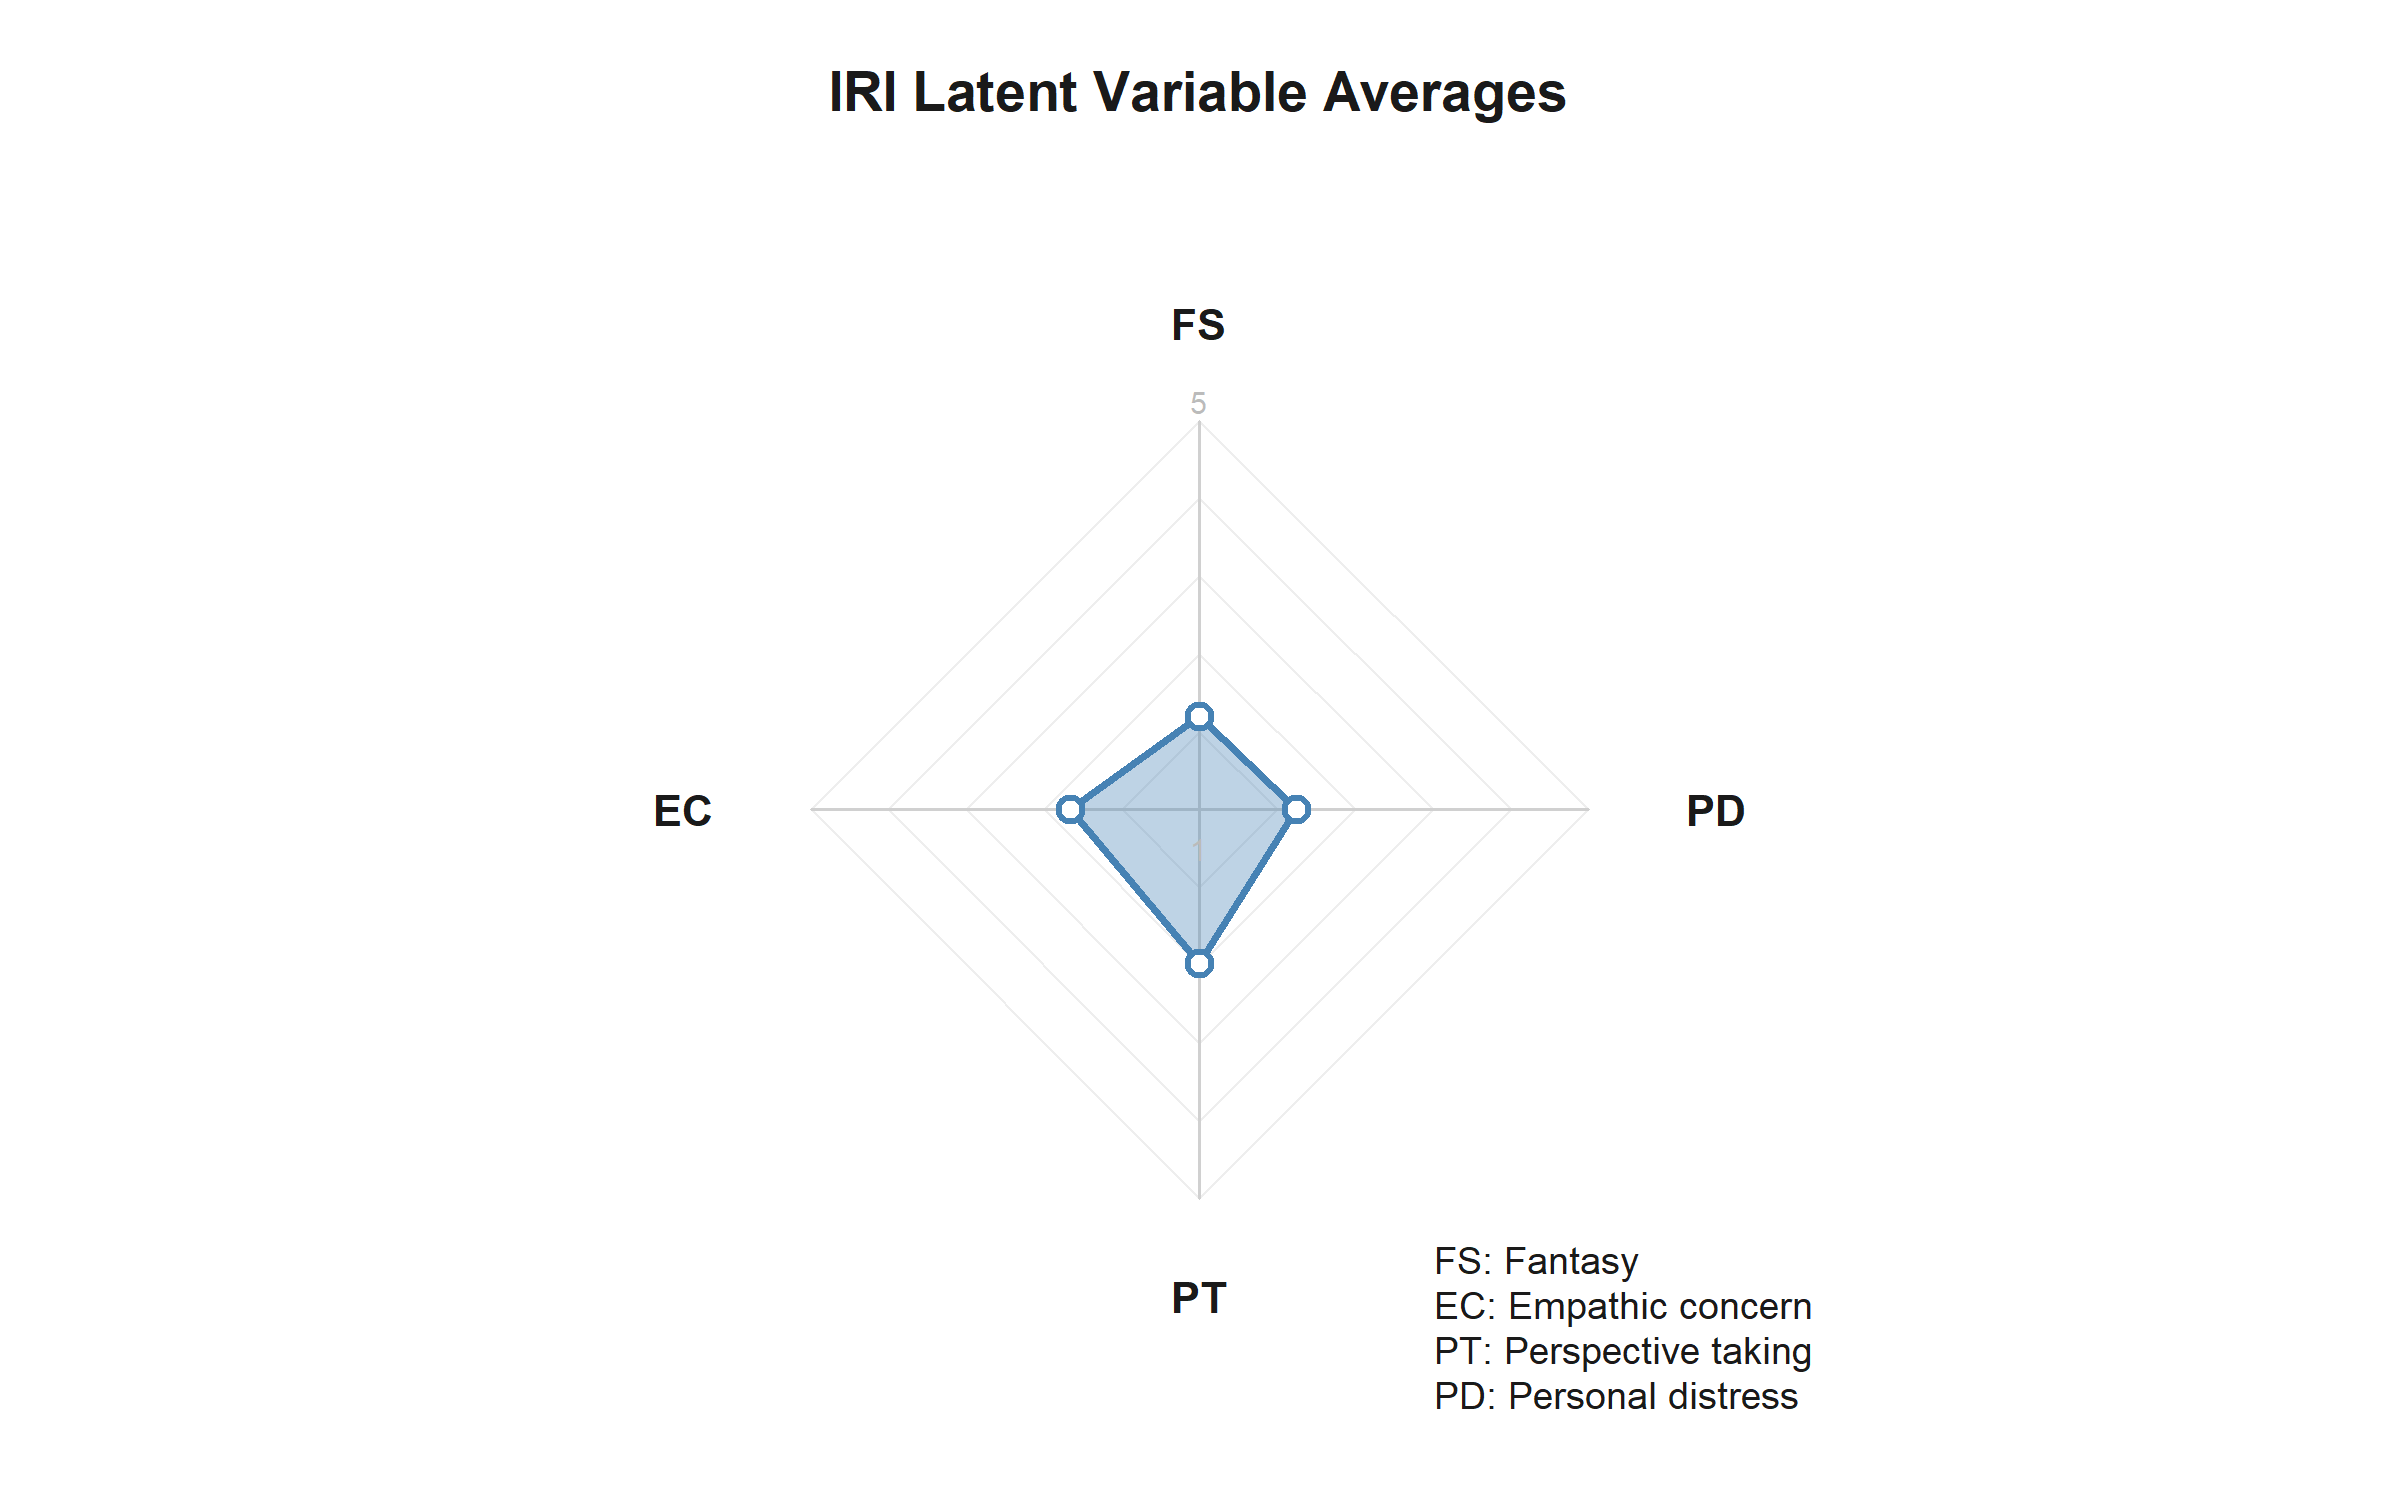
\includegraphics[width=0.92\textwidth]{../figures/figure_03_empathy_radar.png}
\caption{IRI Latent Variable Averages (Radar Plot profile).}
\label{fig:radar}
\end{figure}
Judgment severity distributions segmented by experimental conditions are presented in Figure \ref{fig:dist_panels}.
\begin{figure}[H]
\centering
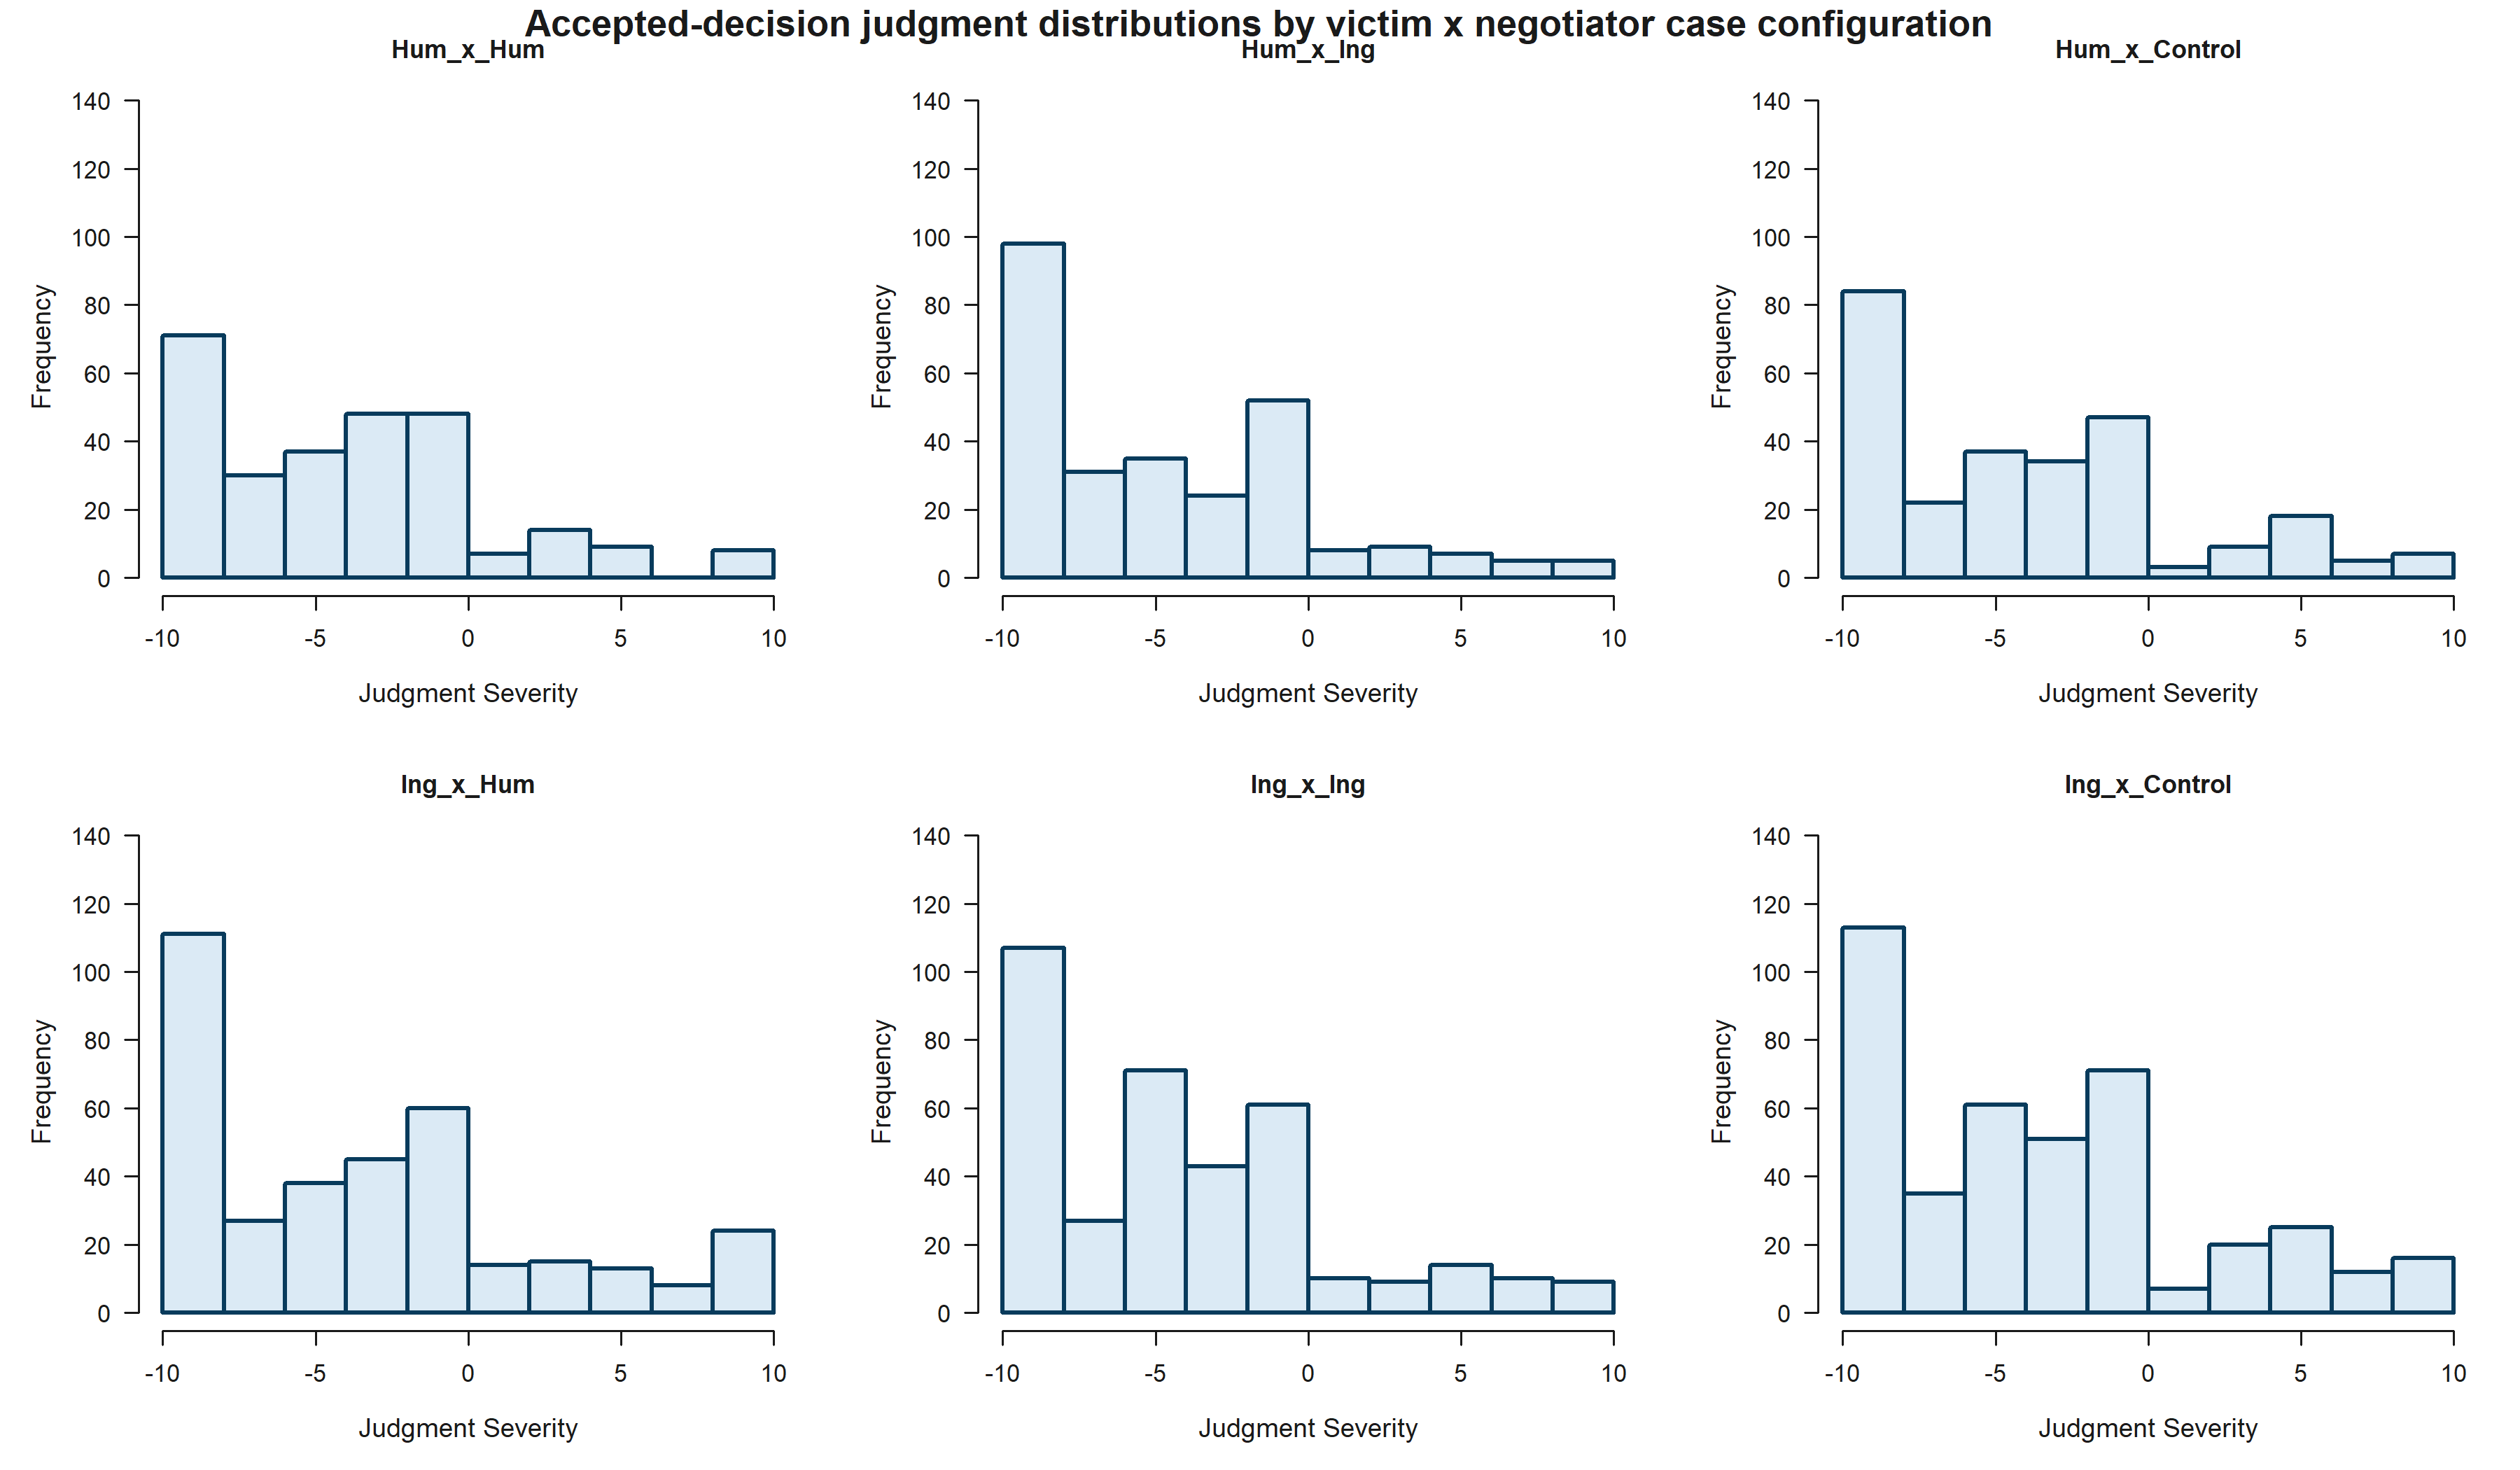
\includegraphics[width=0.92\textwidth]{../figures/figure_04_severity_panels.png}
\caption{Accepted-decision judgment distributions by explicit victim x negotiator case configuration.}
\label{fig:dist_panels}
\end{figure}
\begin{table}[H]
\centering
\caption{Observed judgment summaries across explicit victim x negotiator case configurations, participant role, and decision context.}
\label{tab:case_configuration_summary}
\resizebox{\textwidth}{!}{%
\begin{tabular}{lllllllll}
\toprule
case\_configuration & role & decision\_accept & Observations & MeanJudgement & SDJudgement & SEJudgement & Lower95 & Upper95 \\
\midrule
Hum\_x\_Control & observer & 0 & 168 & 6.417 & 4.066 & 0.314 & 5.802 & 7.032 \\
Hum\_x\_Hum & observer & 0 & 142 & 6.873 & 3.496 & 0.293 & 6.298 & 7.448 \\
Hum\_x\_Ing & observer & 0 & 157 & 6.172 & 3.558 & 0.284 & 5.615 & 6.728 \\
Ing\_x\_Control & observer & 0 & 192 & 6.547 & 3.410 & 0.246 & 6.064 & 7.029 \\
Ing\_x\_Hum & observer & 0 & 169 & 5.757 & 4.510 & 0.347 & 5.077 & 6.437 \\
Ing\_x\_Ing & observer & 0 & 187 & 6.636 & 3.601 & 0.263 & 6.120 & 7.152 \\
Hum\_x\_Control & victim & 0 & 136 & 6.088 & 4.153 & 0.356 & 5.390 & 6.786 \\
Hum\_x\_Hum & victim & 0 & 143 & 5.259 & 4.616 & 0.386 & 4.502 & 6.015 \\
Hum\_x\_Ing & victim & 0 & 116 & 6.534 & 3.559 & 0.330 & 5.887 & 7.182 \\
Ing\_x\_Control & victim & 0 & 207 & 6.744 & 3.696 & 0.257 & 6.241 & 7.247 \\
Ing\_x\_Hum & victim & 0 & 215 & 6.637 & 3.891 & 0.265 & 6.117 & 7.157 \\
Ing\_x\_Ing & victim & 0 & 209 & 7.005 & 3.575 & 0.247 & 6.520 & 7.490 \\
Hum\_x\_Control & observer & 1 & 137 & -3.044 & 5.123 & 0.438 & -3.902 & -2.186 \\
Hum\_x\_Hum & observer & 1 & 150 & -3.573 & 4.453 & 0.364 & -4.286 & -2.861 \\
Hum\_x\_Ing & observer & 1 & 148 & -3.757 & 4.972 & 0.409 & -4.558 & -2.956 \\
Ing\_x\_Control & observer & 1 & 173 & -3.012 & 4.767 & 0.362 & -3.722 & -2.301 \\
Ing\_x\_Hum & observer & 1 & 178 & -2.596 & 5.421 & 0.406 & -3.392 & -1.799 \\
Ing\_x\_Ing & observer & 1 & 189 & -3.063 & 4.986 & 0.363 & -3.774 & -2.353 \\
Hum\_x\_Control & victim & 1 & 129 & -4.054 & 4.931 & 0.434 & -4.905 & -3.203 \\
Hum\_x\_Hum & victim & 1 & 122 & -3.434 & 4.846 & 0.439 & -4.294 & -2.574 \\
Hum\_x\_Ing & victim & 1 & 126 & -4.825 & 4.427 & 0.394 & -5.598 & -4.052 \\
Ing\_x\_Control & victim & 1 & 238 & -2.824 & 5.658 & 0.367 & -3.542 & -2.105 \\
Ing\_x\_Hum & victim & 1 & 177 & -3.424 & 5.606 & 0.421 & -4.250 & -2.598 \\
Ing\_x\_Ing & victim & 1 & 172 & -4.250 & 4.678 & 0.357 & -4.949 & -3.551 \\
\bottomrule
\end{tabular}
}
\end{table}

\section{Bi-variate Statistics}
The correlation matrix between the psychometric subscales and the mean moral judgment is presented below.
\begin{table}[H]
\centering
\caption{Correlation Matrix: IRI Subscales and Moral Judgment.}
\label{tab:bivar}
\resizebox{\textwidth}{!}{%
\begin{tabular}{llllll}
\toprule
Fantasy & Empathic Concern & Perspective Taking & Personal Distress & Total IRI & Mean Judgment \\
\midrule
1.000 & 0.500 & 0.554 & 0.509 & 0.830 & -0.030 \\
0.500 & 1.000 & 0.424 & 0.649 & 0.818 & -0.116 \\
0.554 & 0.424 & 1.000 & 0.301 & 0.730 & 0.074 \\
0.509 & 0.649 & 0.301 & 1.000 & 0.762 & -0.010 \\
0.830 & 0.818 & 0.730 & 0.762 & 1.000 & -0.029 \\
-0.030 & -0.116 & 0.074 & -0.010 & -0.029 & 1.000 \\
\bottomrule
\end{tabular}
}
\end{table}
Visual representations of these relationships are provided in Figure \ref{fig:bivar_scatters}.
\begin{figure}[H]
\centering
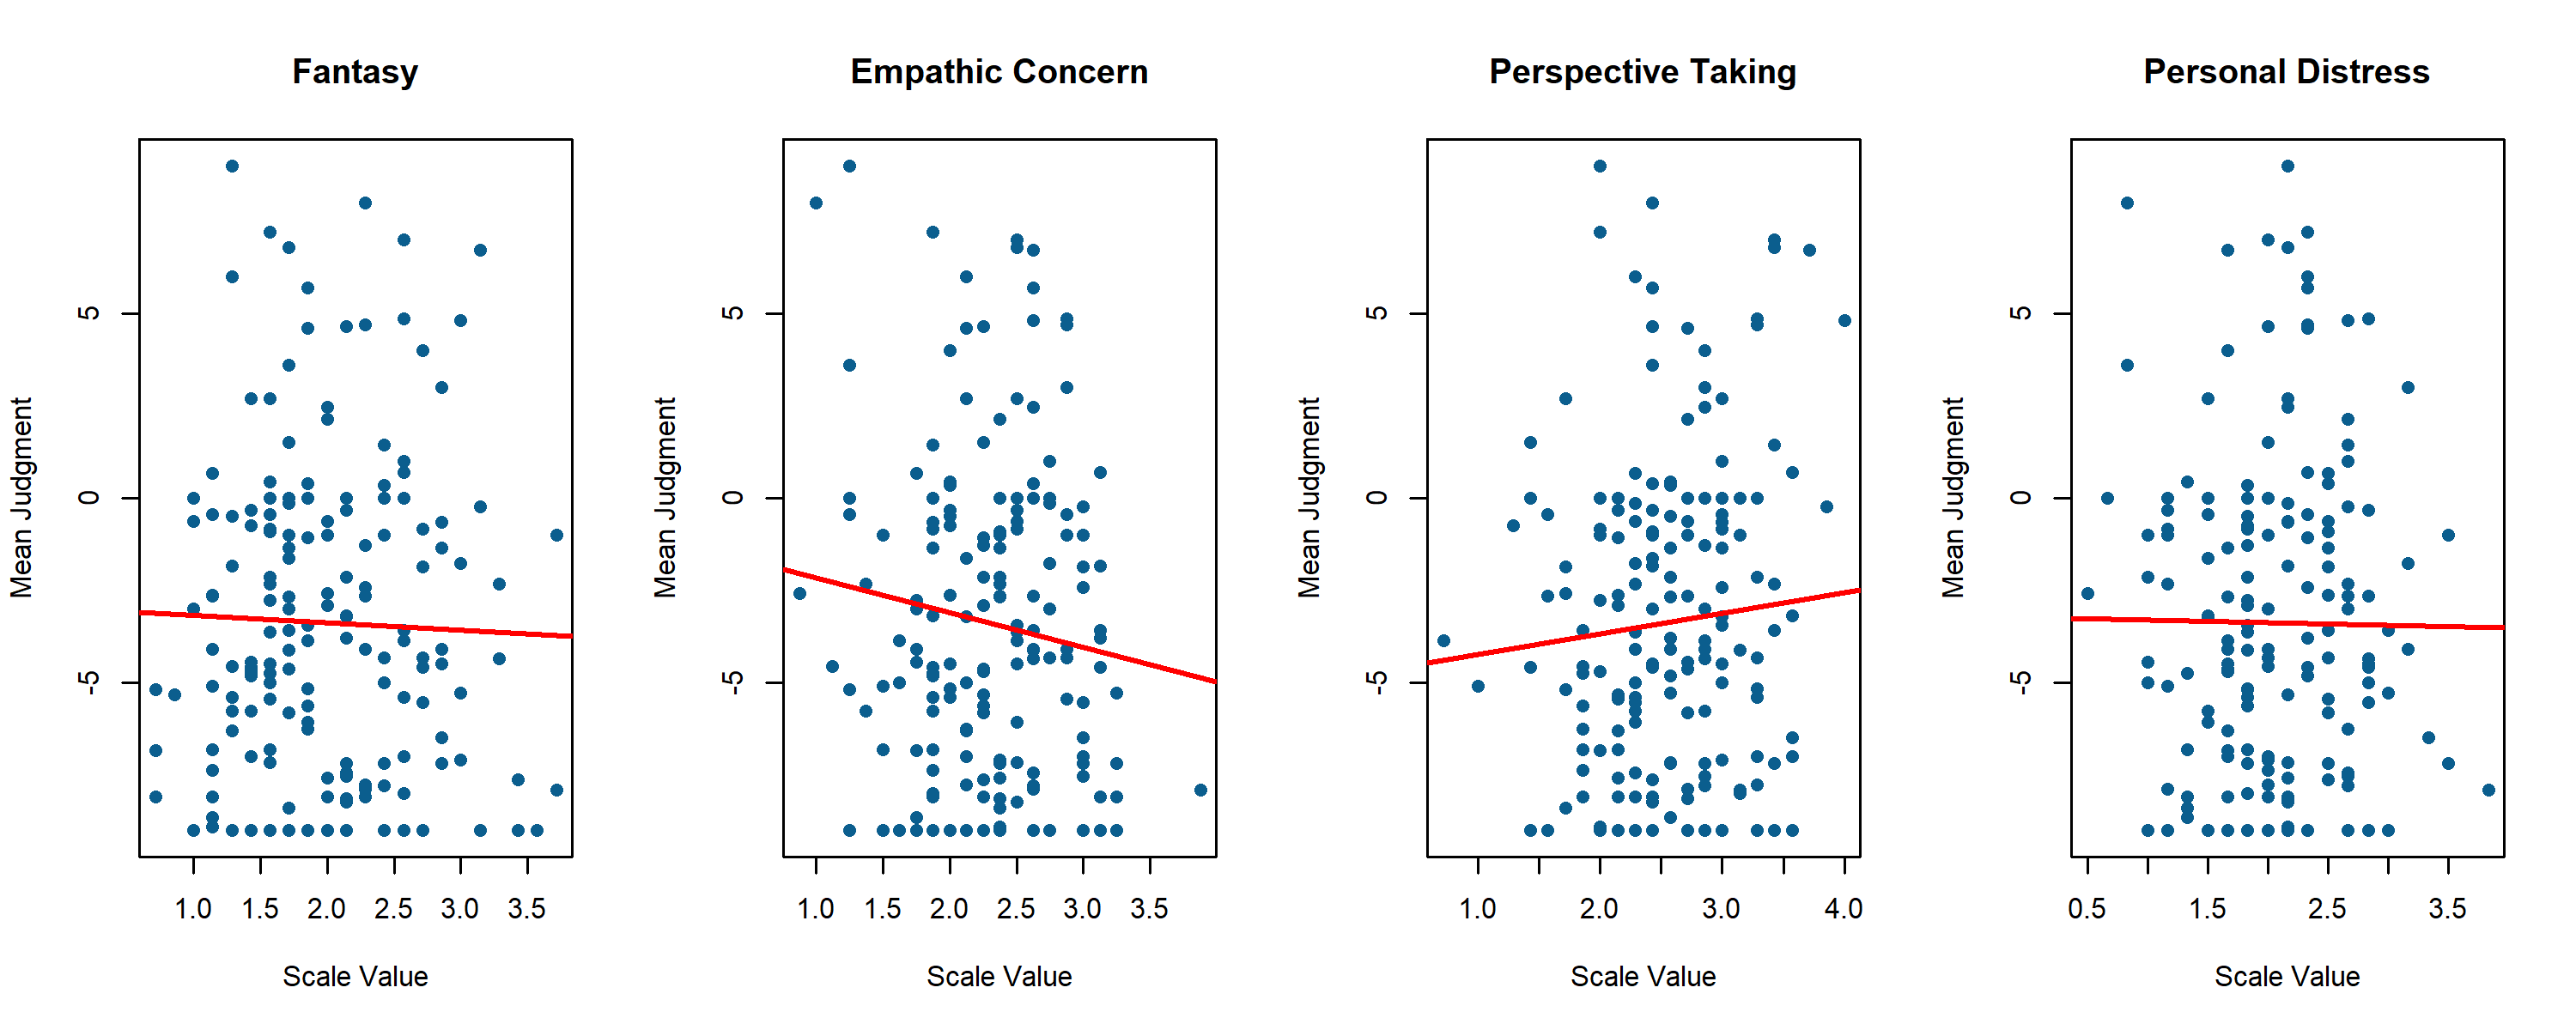
\includegraphics[width=0.92\textwidth]{../figures/figure_05_bivariate_scatters.png}
\caption{Bivariate Scatters: IRI Scales vs. Mean Judgment.}
\label{fig:bivar_scatters}
\end{figure}

\section{Estimator Fit Summary}
The following table consolidates the fit-status information for the primary Tobit models and the non-parametric robustness branch. In the default pipeline, participant-level cluster bootstrap launches immediately after a converged full-sample non-parametric fit is available; if bootstrap is disabled manually or too few bootstrap refits converge, that status is shown explicitly.
\begin{table}[H]
\centering
\caption{Estimator fit summary across Tobit and cluster-aware non-parametric specifications.}
\label{tab:model_fit_summary}
\resizebox{\textwidth}{!}{%
\begin{tabular}{llllllllll}
\toprule
Model & Approach & Status & Converged & Iterations & BootstrapReplicates & BootstrapSuccessful & Observations & Participants & ClusterUnit \\
\midrule
H1\_A\_Total\_CLAD & CLAD & not\_converged & FALSE & 2000 & 1 & NA & 1939 & 199 & id \\
H1\_B\_Constructs\_CLAD & CLAD & failed & FALSE & NA & 1 & 0 & 1939 & 199 & id \\
H2a\_A\_Total\_CLAD & CLAD & bootstrap\_sparse & TRUE & 46 & 1 & 1 & 1262 & 199 & id \\
H2a\_B\_Constructs\_CLAD & CLAD & failed & FALSE & NA & 1 & 0 & 1262 & 199 & id \\
H2b\_A\_Total\_CLAD & CLAD & not\_converged & FALSE & 2000 & 1 & NA & 1939 & 199 & id \\
H2b\_B\_Constructs\_CLAD & CLAD & failed & FALSE & NA & 1 & 0 & 1939 & 199 & id \\
H3\_A\_Total\_CLAD & CLAD & not\_converged & FALSE & 2000 & 1 & NA & 1939 & 199 & id \\
H3\_B\_Constructs\_CLAD & CLAD & not\_converged & FALSE & 2000 & 1 & NA & 1939 & 199 & id \\
H1\_A\_Total\_Tobit & Tobit & completed & NA & 3 & NA & NA & 1939 & 199 & id \\
H1\_B\_Constructs\_Tobit & Tobit & completed & NA & 3 & NA & NA & 1939 & 199 & id \\
H2a\_A\_Total\_Tobit & Tobit & completed & NA & 3 & NA & NA & 1262 & 199 & id \\
H2a\_B\_Constructs\_Tobit & Tobit & completed & NA & 3 & NA & NA & 1262 & 199 & id \\
H2b\_A\_Total\_Tobit & Tobit & completed & NA & 3 & NA & NA & 1939 & 199 & id \\
H2b\_B\_Constructs\_Tobit & Tobit & completed & NA & 3 & NA & NA & 1939 & 199 & id \\
H3\_A\_Total\_Tobit & Tobit & completed & NA & 3 & NA & NA & 1939 & 199 & id \\
H3\_B\_Constructs\_Tobit & Tobit & completed & NA & 3 & NA & NA & 1939 & 199 & id \\
\bottomrule
\end{tabular}
}
\end{table}

\subsection{Hypothesis Significance Summary}
The following concise table lists only hypothesis-relevant predictors that reached at least p < 0.10, using conventional symbols to indicate strength of evidence. If the non-parametric bootstrap is disabled, too sparse, or the censored median fit does not converge, the non-parametric column reports that status instead of inferential symbols. Dynamic figures are generated only for predictors that appear in this table with at least one significance symbol.
\begin{table}[H]
\centering
\caption{Hypothesis-level significance summary across Tobit and cluster-aware non-parametric models.}
\label{tab:hypothesis_summary}
\resizebox{\textwidth}{!}{%
\begin{tabular}{lll}
\toprule
Hypothesis & Tobit significant predictors & Non-parametric significant predictors \\
\midrule
Higher empathy predicts lower moral-judgment scores for harmful decisions after conditioning on explicit victim x negotiator case configurations. & Empathy: Empathic concern*; Empathy: Perspective taking* & None \\
Same-faculty and cross-faculty betrayal cases are evaluated through explicit victim x negotiator configurations rather than a single same\_group\_harm flag. & Case configuration: Humanities victim x Engineering negotiator+ & Bootstrap too sparse \\
Relational judgments are interpreted through explicit victim x negotiator case configurations such as Hum\_x\_Ing, Hum\_x\_Control, Ing\_x\_Hum, Ing\_x\_Ing, and Ing\_x\_Control. & Case configuration: Humanities victim x Engineering negotiator+ & None \\
The empathy effect may vary across explicit victim x negotiator pairings, so moderation is modeled through empathy interactions with case-configuration contrasts. & Case configuration: Engineering victim x Humanities negotiator x Empathy: Empathic concern**; Case configuration: Engineering victim x Humanities negotiator x Empathy: Personal distress*; Case configuration: Humanities victim x Engineering negotiator x Empathy composite (average)*; Case configuration: Engineering victim x Control label hidden negotiator x Empathy: Empathic concern+; Case configuration: Engineering victim x Humanities negotiator x Empathy composite (average)+ & None \\
\bottomrule
\end{tabular}
}
\end{table}

\subsection{Significance-Driven Figures}
Only hypothesis-relevant predictors that reach p < 0.10 or better are visualized automatically. These dynamic figures use the saved Tobit and clustered non-parametric outputs, and participant id remains only an inference-level clustering unit rather than a substantive explanatory variable.

\paragraph{H1: Empathy under explicit case configuration}

Empathy: Empathic concern is statistically significant in the Tobit model (*, p = 0.025). Figure \ref{fig:sig_H1_iri_ec} shows that across the observed range, higher Empathy: Empathic concern corresponds to lower predicted latent judgment.

\begin{figure}[H]
\centering
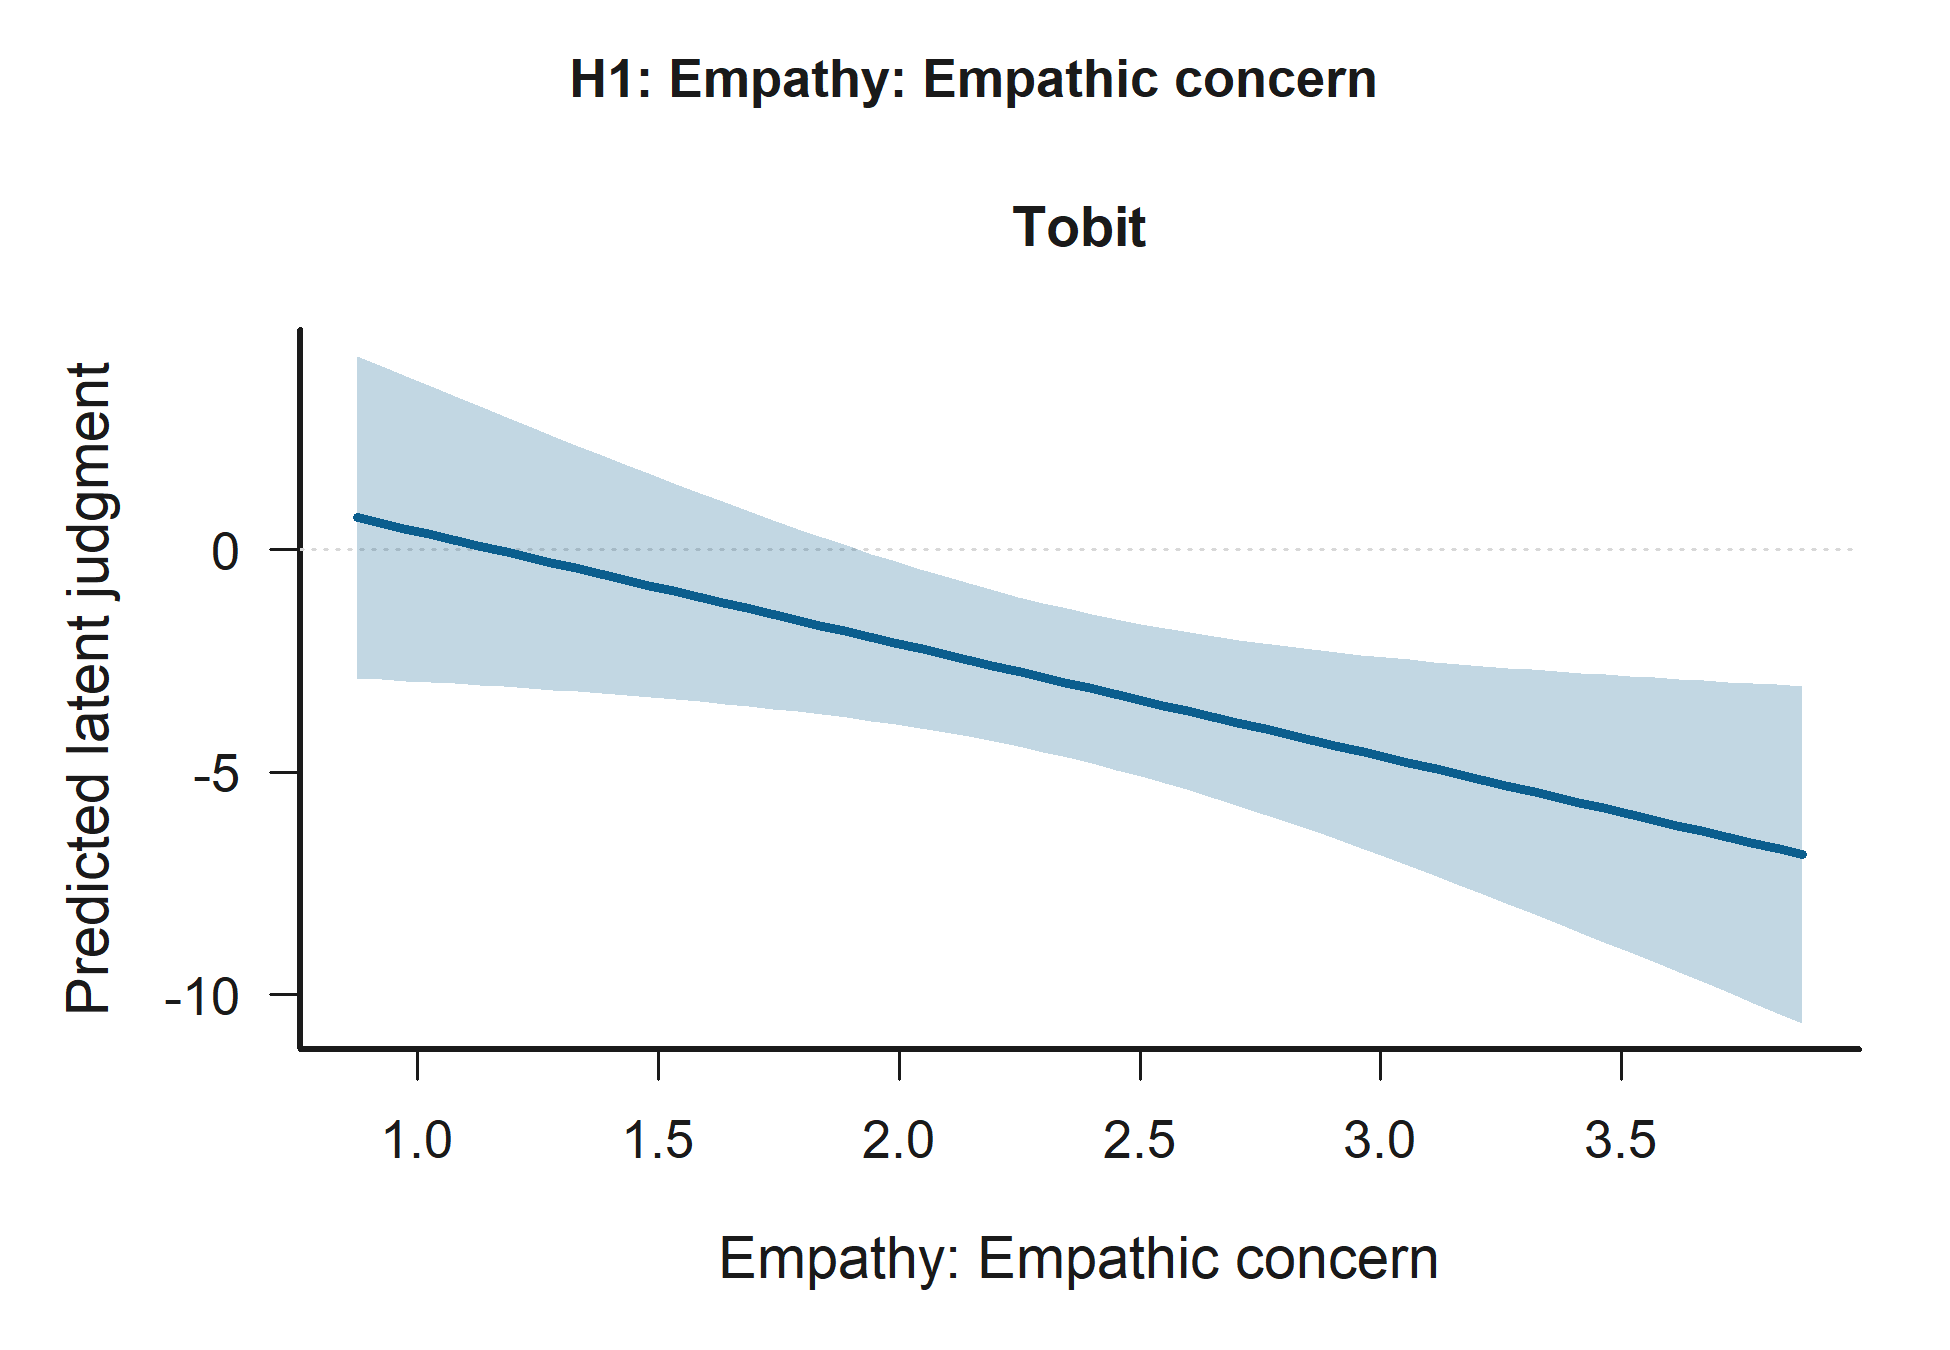
\includegraphics[width=0.92\textwidth]{../figures/figure_sig_H1_iri_ec.png}
\caption{Effect Plot for Empathy: Empathic concern in H1: Empathy under explicit case configuration. Support comes from the Tobit model (*, p = 0.025). The panels show predicted latent judgments with 95\% confidence intervals.}
\label{fig:sig_H1_iri_ec}
\end{figure}

Empathy: Perspective taking is statistically significant in the Tobit model (*, p = 0.042). Figure \ref{fig:sig_H1_iri_pt} shows that across the observed range, higher Empathy: Perspective taking corresponds to higher predicted latent judgment.

\begin{figure}[H]
\centering
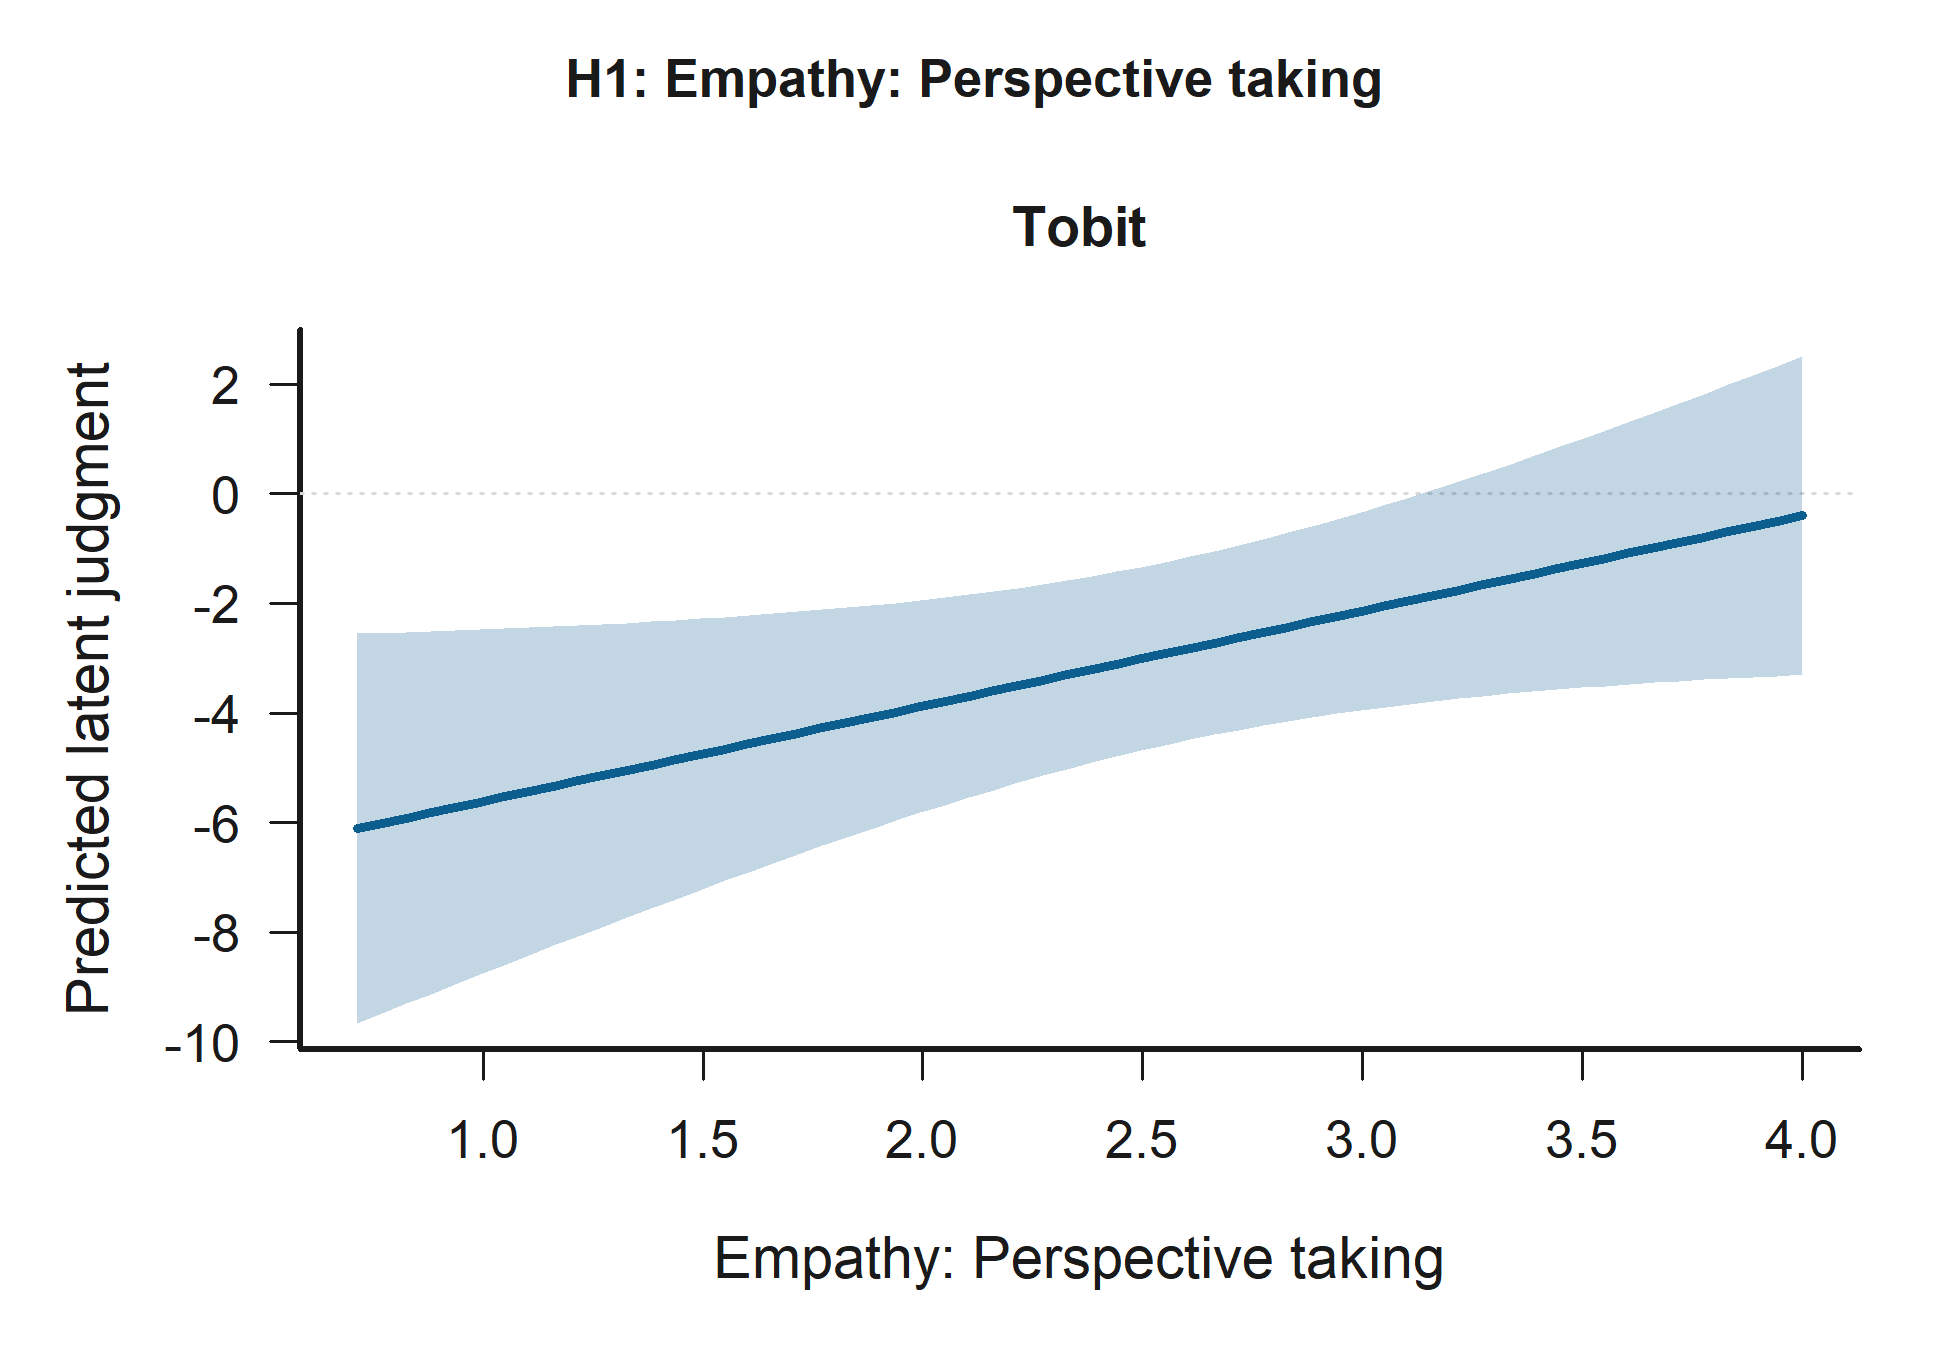
\includegraphics[width=0.92\textwidth]{../figures/figure_sig_H1_iri_pt.png}
\caption{Effect Plot for Empathy: Perspective taking in H1: Empathy under explicit case configuration. Support comes from the Tobit model (*, p = 0.042). The panels show predicted latent judgments with 95\% confidence intervals.}
\label{fig:sig_H1_iri_pt}
\end{figure}

\paragraph{H2a: Relational betrayal contrasts}

Case configuration: Humanities victim x Engineering negotiator is statistically significant in the Tobit model (+, p = 0.061). Figure \ref{fig:sig_H2a_case_hum_x_ing} shows that predicted latent judgment is lower for Humanities victim x Engineering negotiator than for All other case configurations.

\begin{figure}[H]
\centering
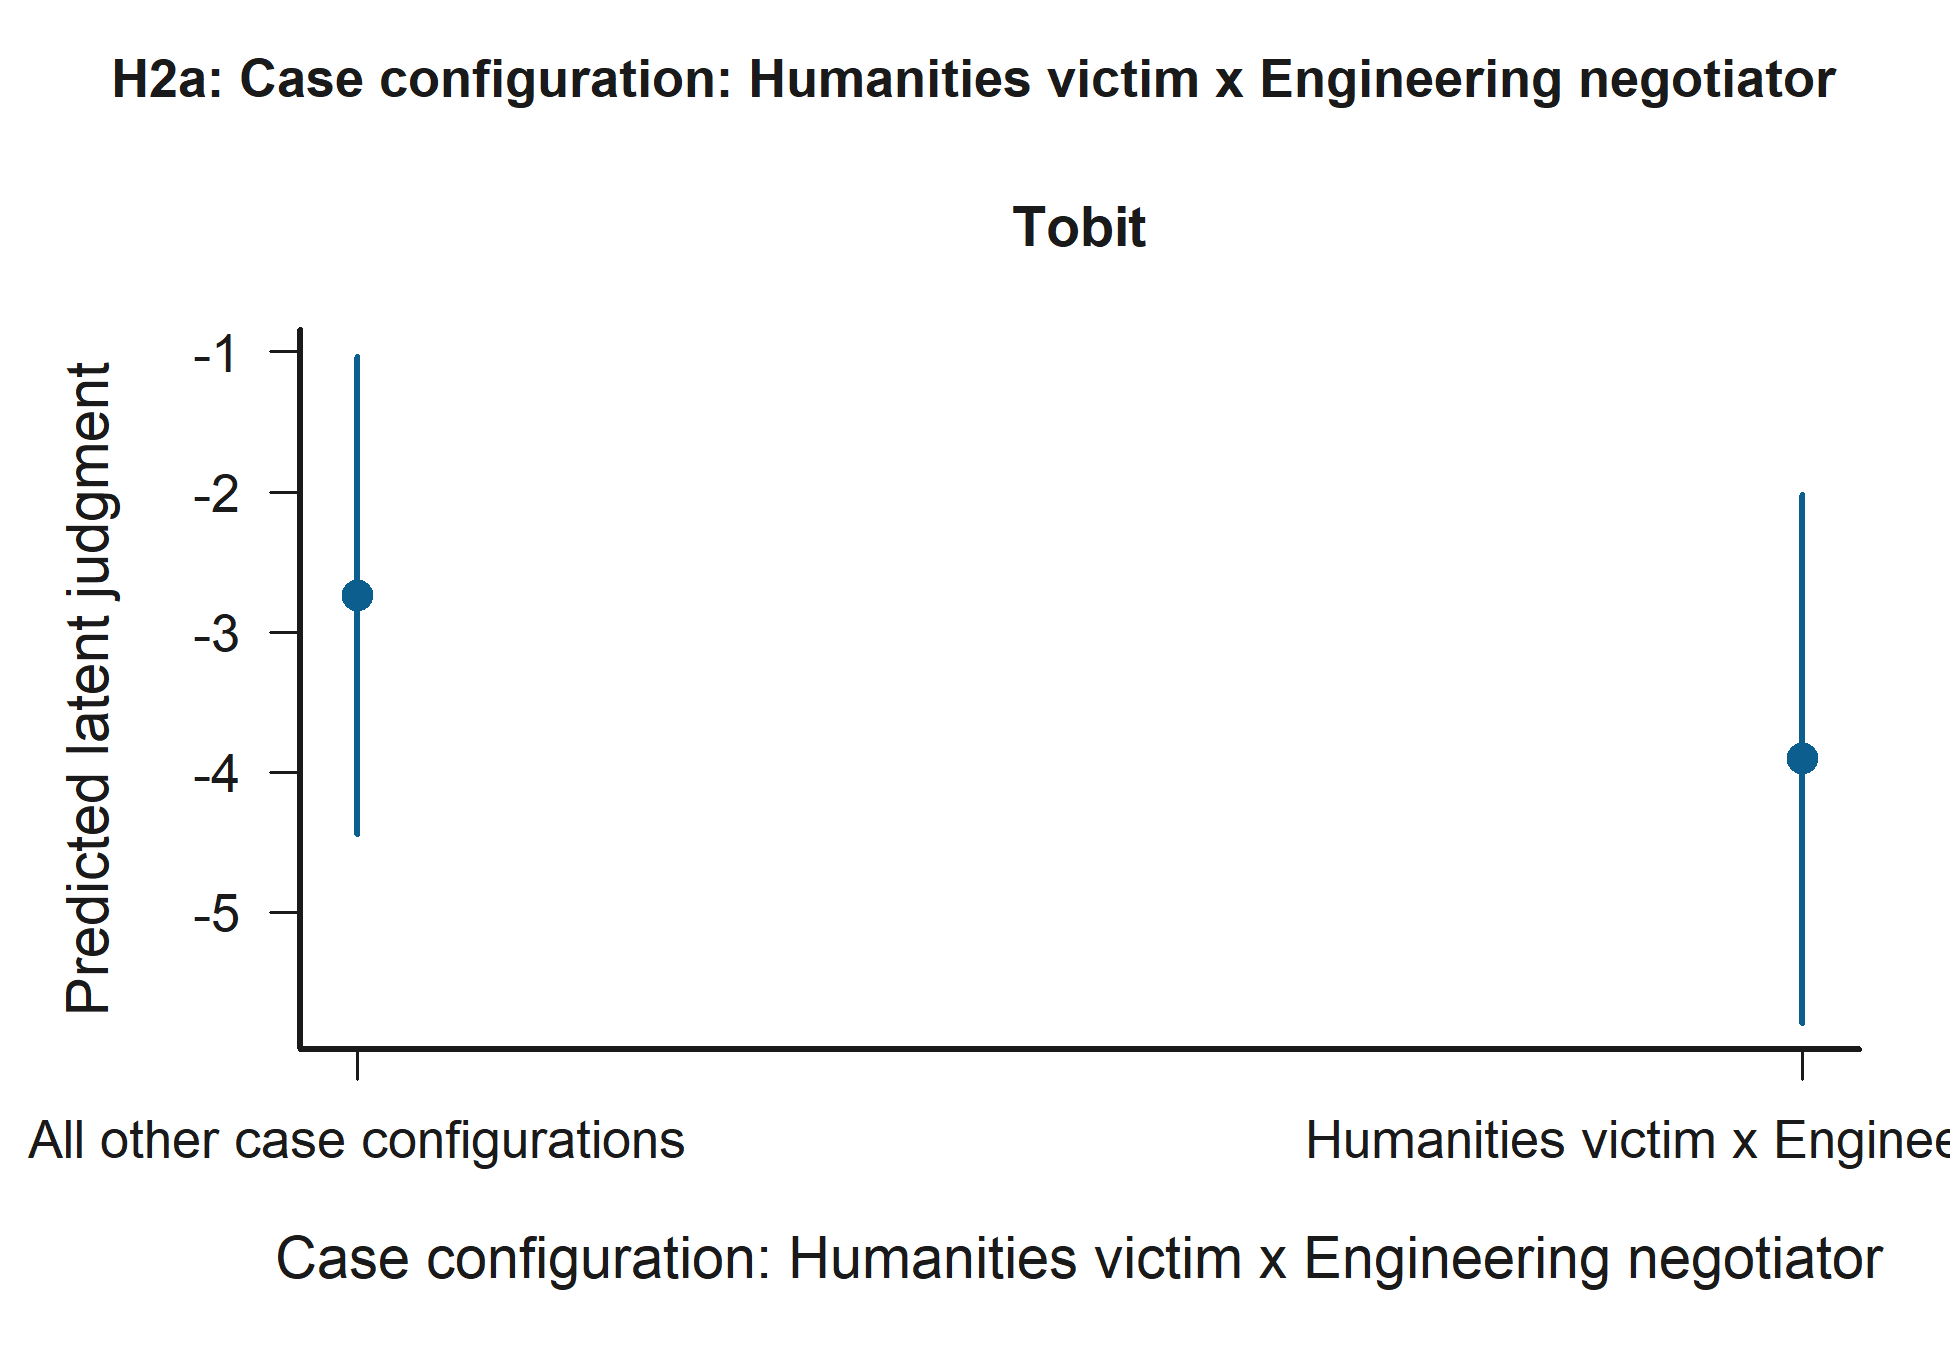
\includegraphics[width=0.92\textwidth]{../figures/figure_sig_H2a_case_hum_x_ing.png}
\caption{Grouped Prediction Plot for Case configuration: Humanities victim x Engineering negotiator in H2a: Relational betrayal contrasts. Support comes from the Tobit model (+, p = 0.061). The panels show predicted latent judgments with 95\% confidence intervals.}
\label{fig:sig_H2a_case_hum_x_ing}
\end{figure}

\paragraph{H2b: Explicit case-configuration contrasts}

Case configuration: Humanities victim x Engineering negotiator is statistically significant in the Tobit model (+, p = 0.065). Figure \ref{fig:sig_H2b_case_hum_x_ing} shows that predicted latent judgment is lower for Humanities victim x Engineering negotiator than for All other case configurations.

\begin{figure}[H]
\centering
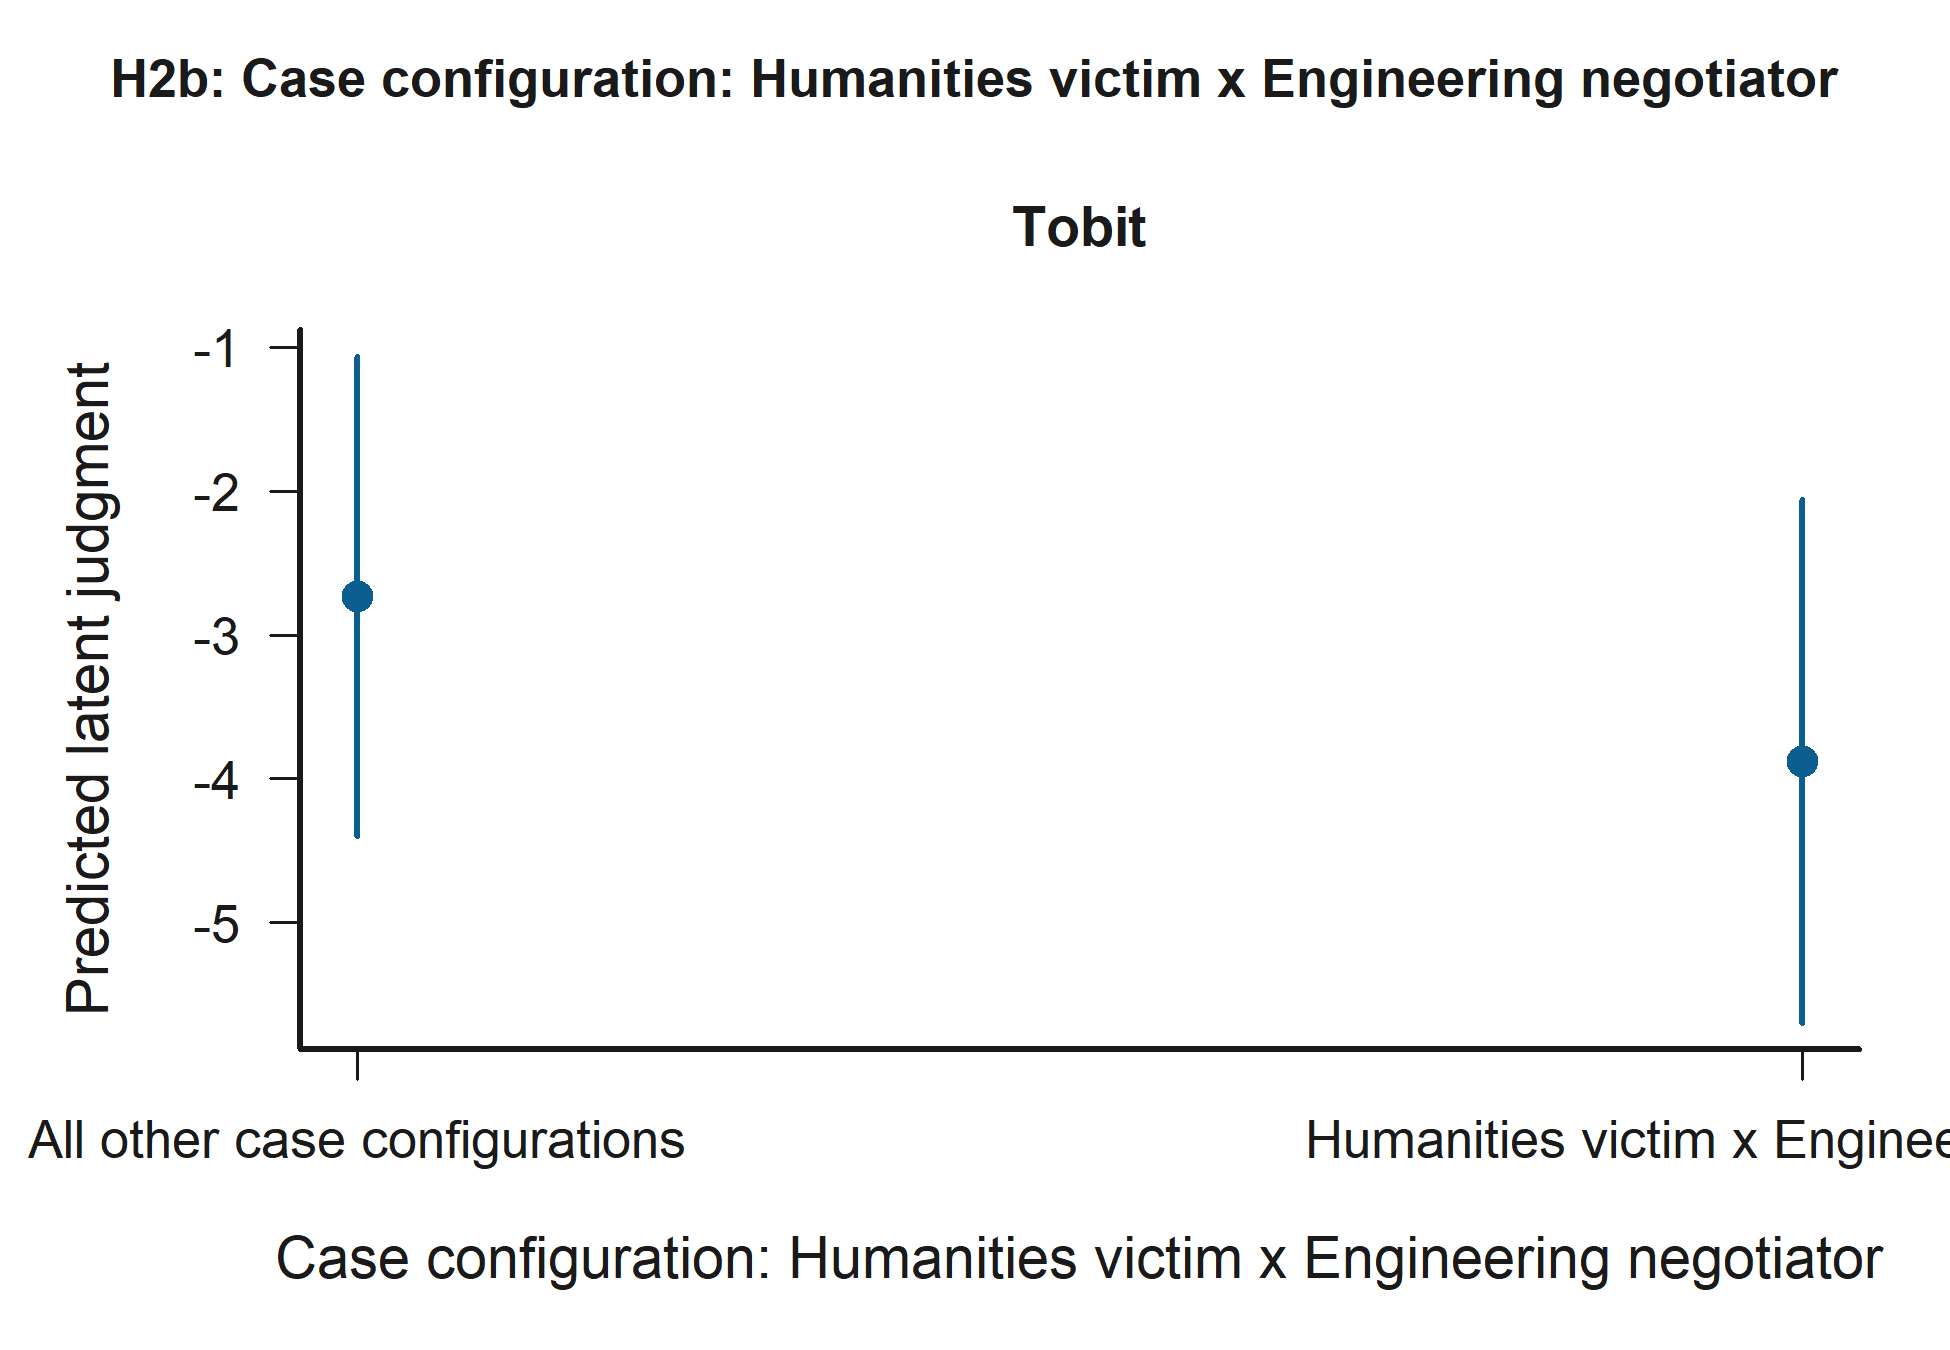
\includegraphics[width=0.92\textwidth]{../figures/figure_sig_H2b_case_hum_x_ing.png}
\caption{Grouped Prediction Plot for Case configuration: Humanities victim x Engineering negotiator in H2b: Explicit case-configuration contrasts. Support comes from the Tobit model (+, p = 0.065). The panels show predicted latent judgments with 95\% confidence intervals.}
\label{fig:sig_H2b_case_hum_x_ing}
\end{figure}

\paragraph{H3: Empathy x case-configuration moderation}

Case configuration: Engineering victim x Humanities negotiator x Empathy: Empathic concern is statistically significant in the Tobit model (**, p < 0.001). Figure \ref{fig:sig_H3_case_ing_x_hum_iri_ec} shows that the predicted relationship falls most sharply for Empathy: Empathic concern when the condition is Engineering victim x Humanities negotiator.

\begin{figure}[H]
\centering
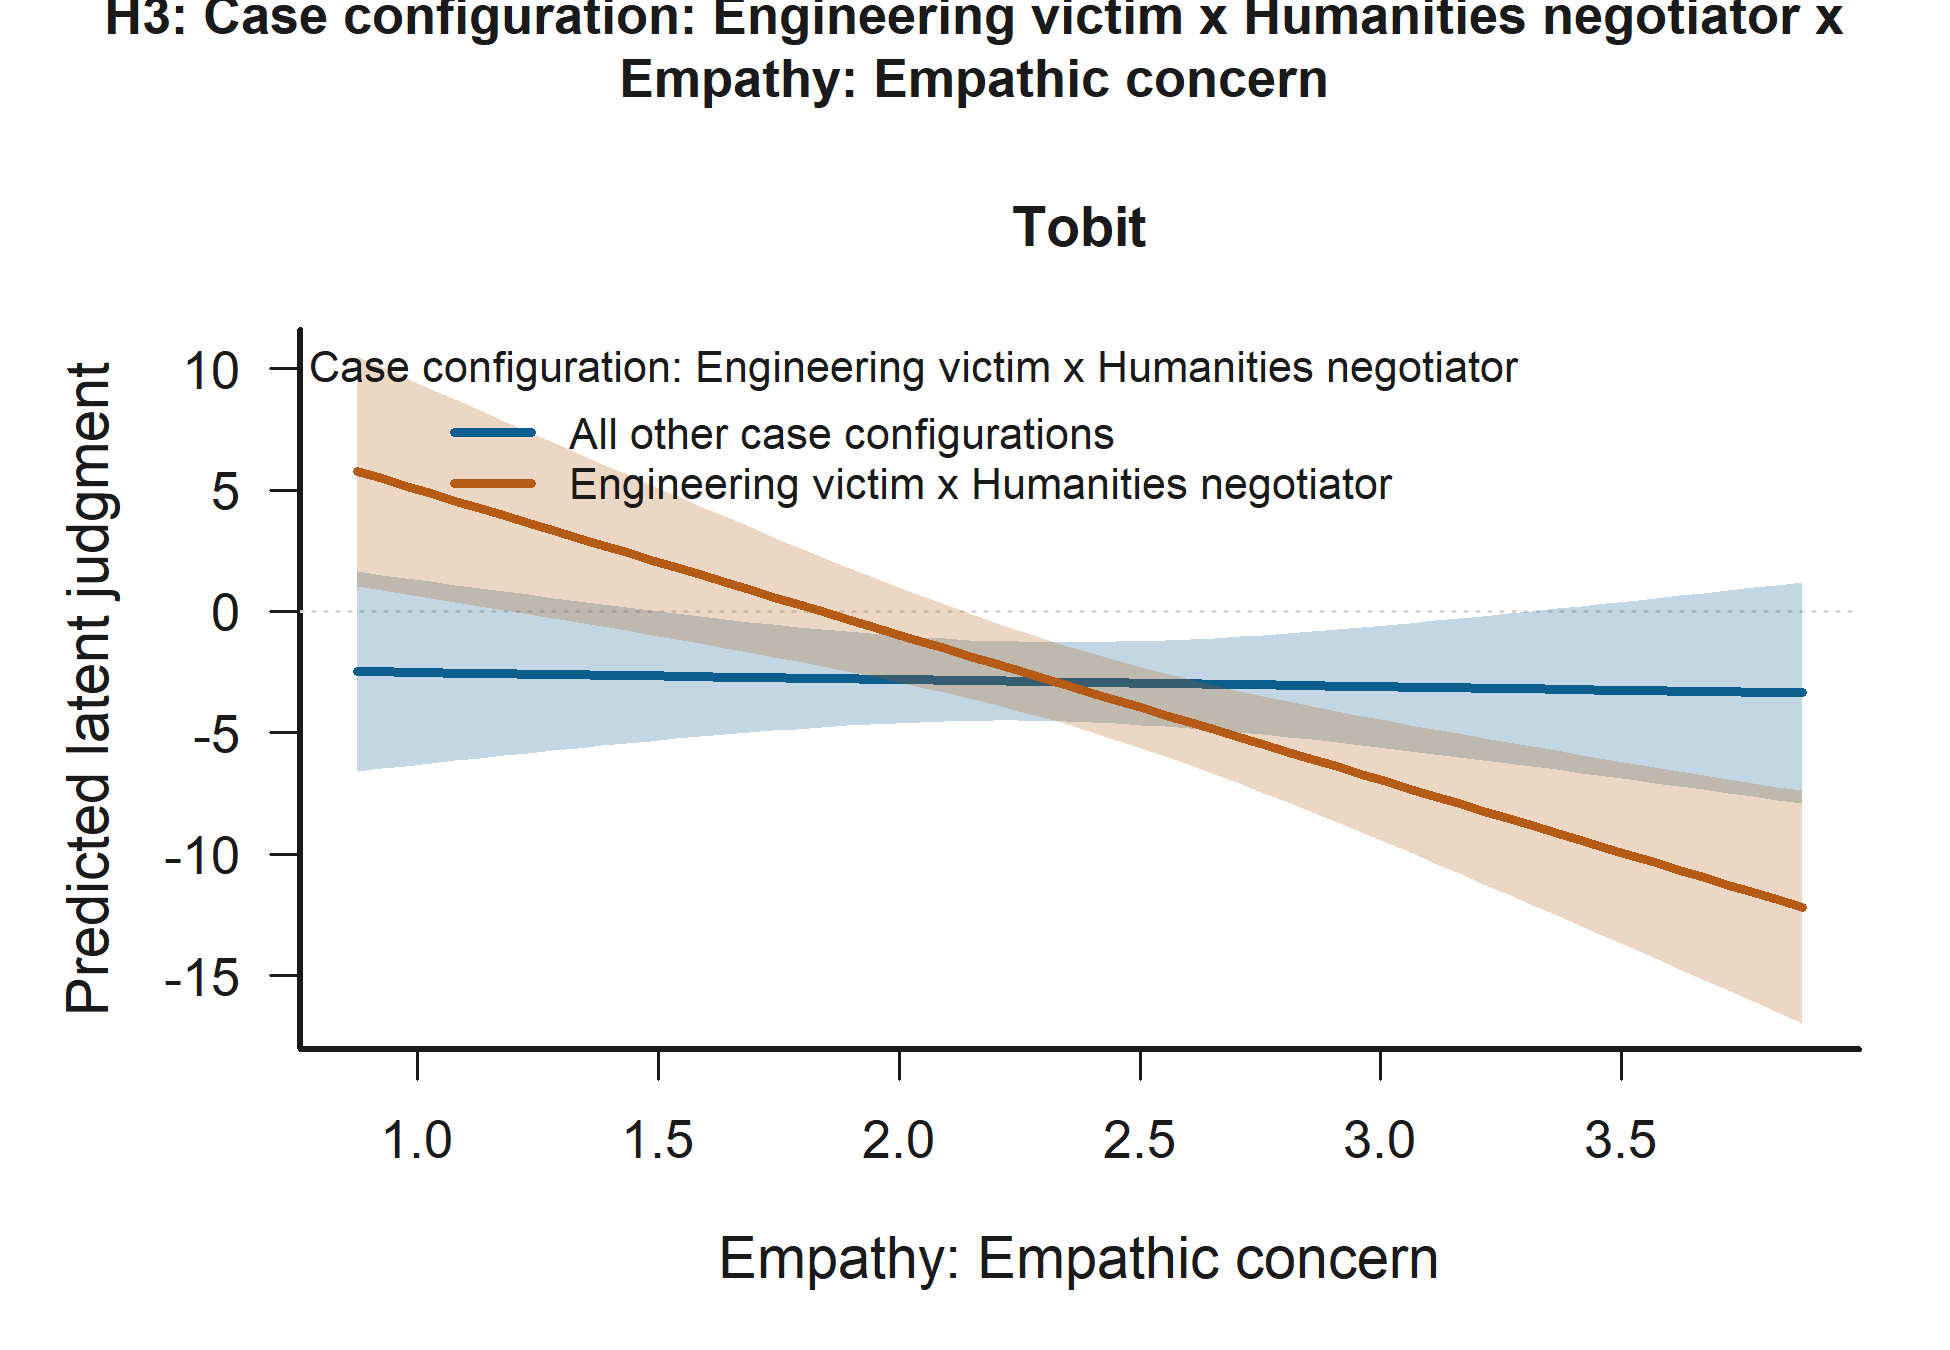
\includegraphics[width=0.92\textwidth]{../figures/figure_sig_H3_case_ing_x_hum_iri_ec.png}
\caption{Interaction Plot for Case configuration: Engineering victim x Humanities negotiator x Empathy: Empathic concern in H3: Empathy x case-configuration moderation. Support comes from the Tobit model (**, p < 0.001). The panels show predicted latent judgments with 95\% confidence intervals.}
\label{fig:sig_H3_case_ing_x_hum_iri_ec}
\end{figure}

Case configuration: Engineering victim x Humanities negotiator x Empathy: Personal distress is statistically significant in the Tobit model (*, p = 0.015). Figure \ref{fig:sig_H3_case_ing_x_hum_iri_pd} shows that the predicted relationship rises most sharply for Empathy: Personal distress when the condition is Engineering victim x Humanities negotiator.

\begin{figure}[H]
\centering
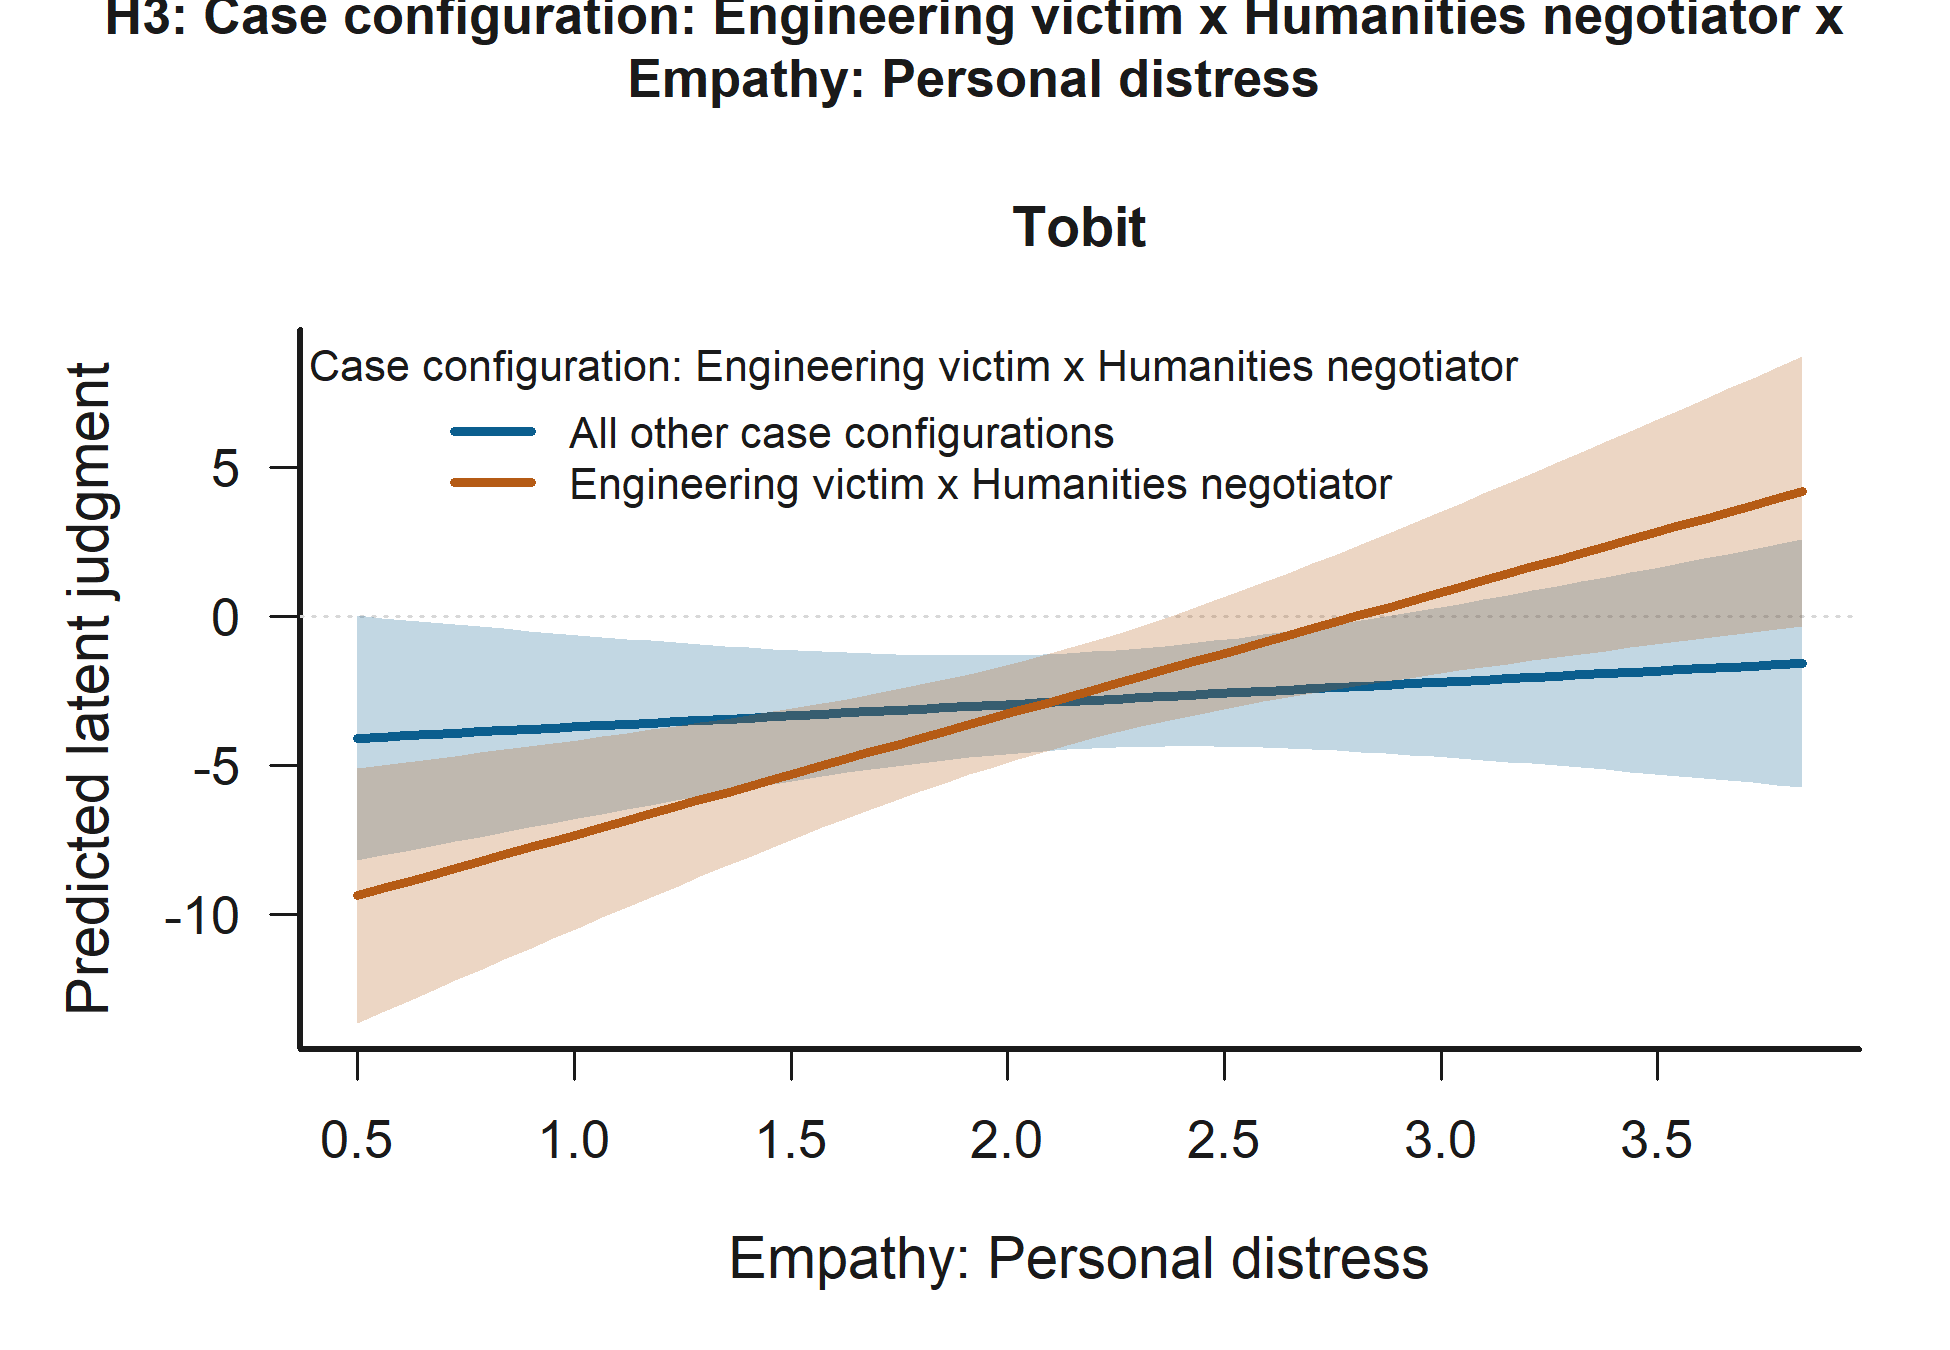
\includegraphics[width=0.92\textwidth]{../figures/figure_sig_H3_case_ing_x_hum_iri_pd.png}
\caption{Interaction Plot for Case configuration: Engineering victim x Humanities negotiator x Empathy: Personal distress in H3: Empathy x case-configuration moderation. Support comes from the Tobit model (*, p = 0.015). The panels show predicted latent judgments with 95\% confidence intervals.}
\label{fig:sig_H3_case_ing_x_hum_iri_pd}
\end{figure}

Case configuration: Humanities victim x Engineering negotiator x Empathy composite (average) is statistically significant in the Tobit model (*, p = 0.049). Figure \ref{fig:sig_H3_case_hum_x_ing_iri_total} shows that the predicted relationship falls most sharply for Empathy composite (average) when the condition is Humanities victim x Engineering negotiator.

\begin{figure}[H]
\centering
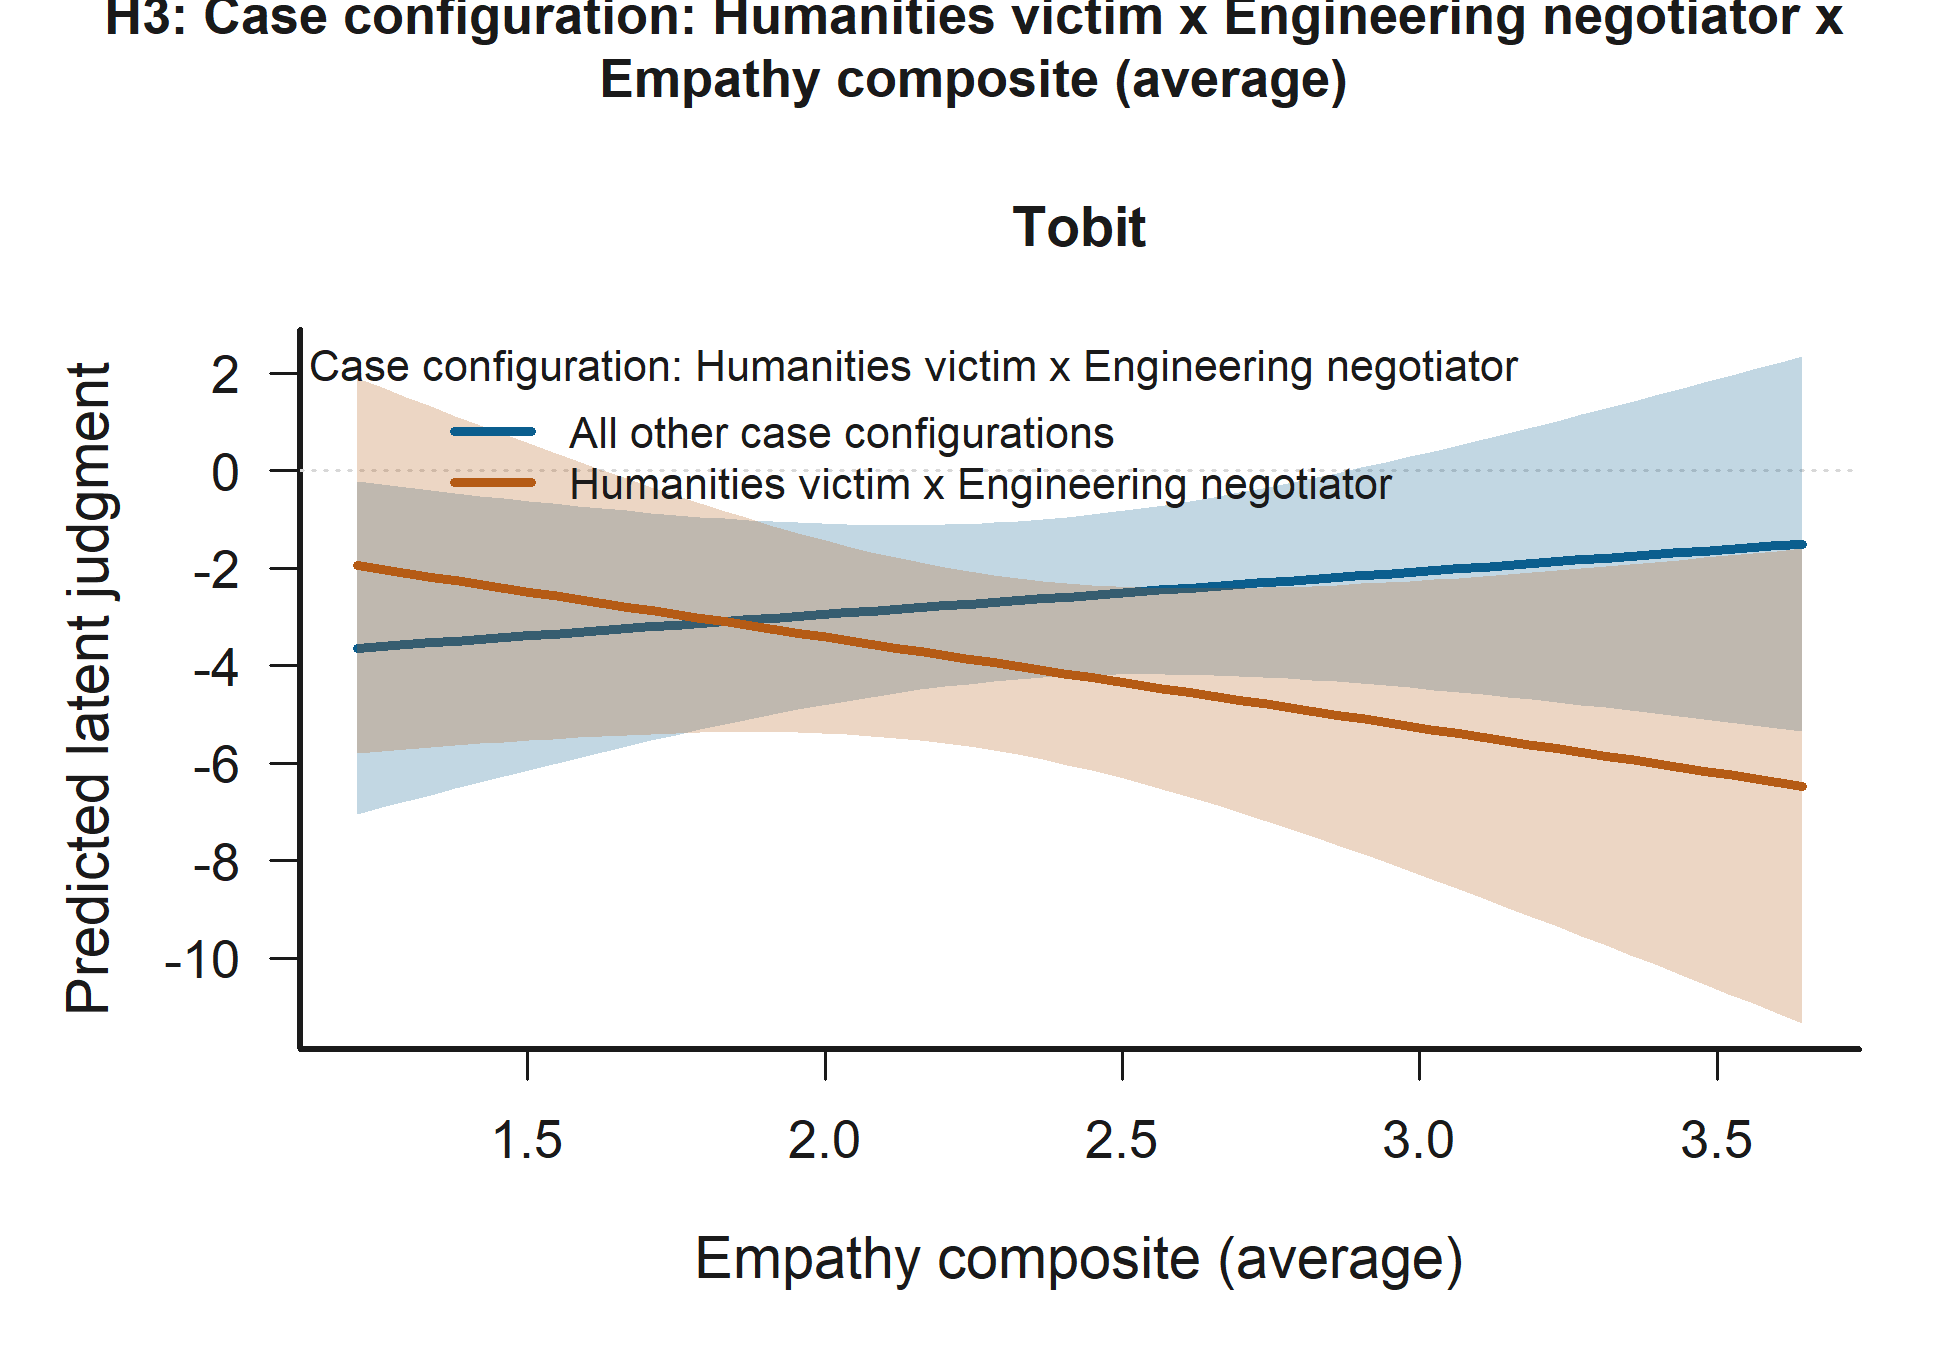
\includegraphics[width=0.92\textwidth]{../figures/figure_sig_H3_case_hum_x_ing_iri_total.png}
\caption{Interaction Plot for Case configuration: Humanities victim x Engineering negotiator x Empathy composite (average) in H3: Empathy x case-configuration moderation. Support comes from the Tobit model (*, p = 0.049). The panels show predicted latent judgments with 95\% confidence intervals.}
\label{fig:sig_H3_case_hum_x_ing_iri_total}
\end{figure}

Case configuration: Engineering victim x Control label hidden negotiator x Empathy: Empathic concern is statistically significant in the Tobit model (+, p = 0.055). Figure \ref{fig:sig_H3_case_ing_x_control_iri_ec} shows that the predicted relationship falls most sharply for Empathy: Empathic concern when the condition is Engineering victim x Control label hidden negotiator.

\begin{figure}[H]
\centering
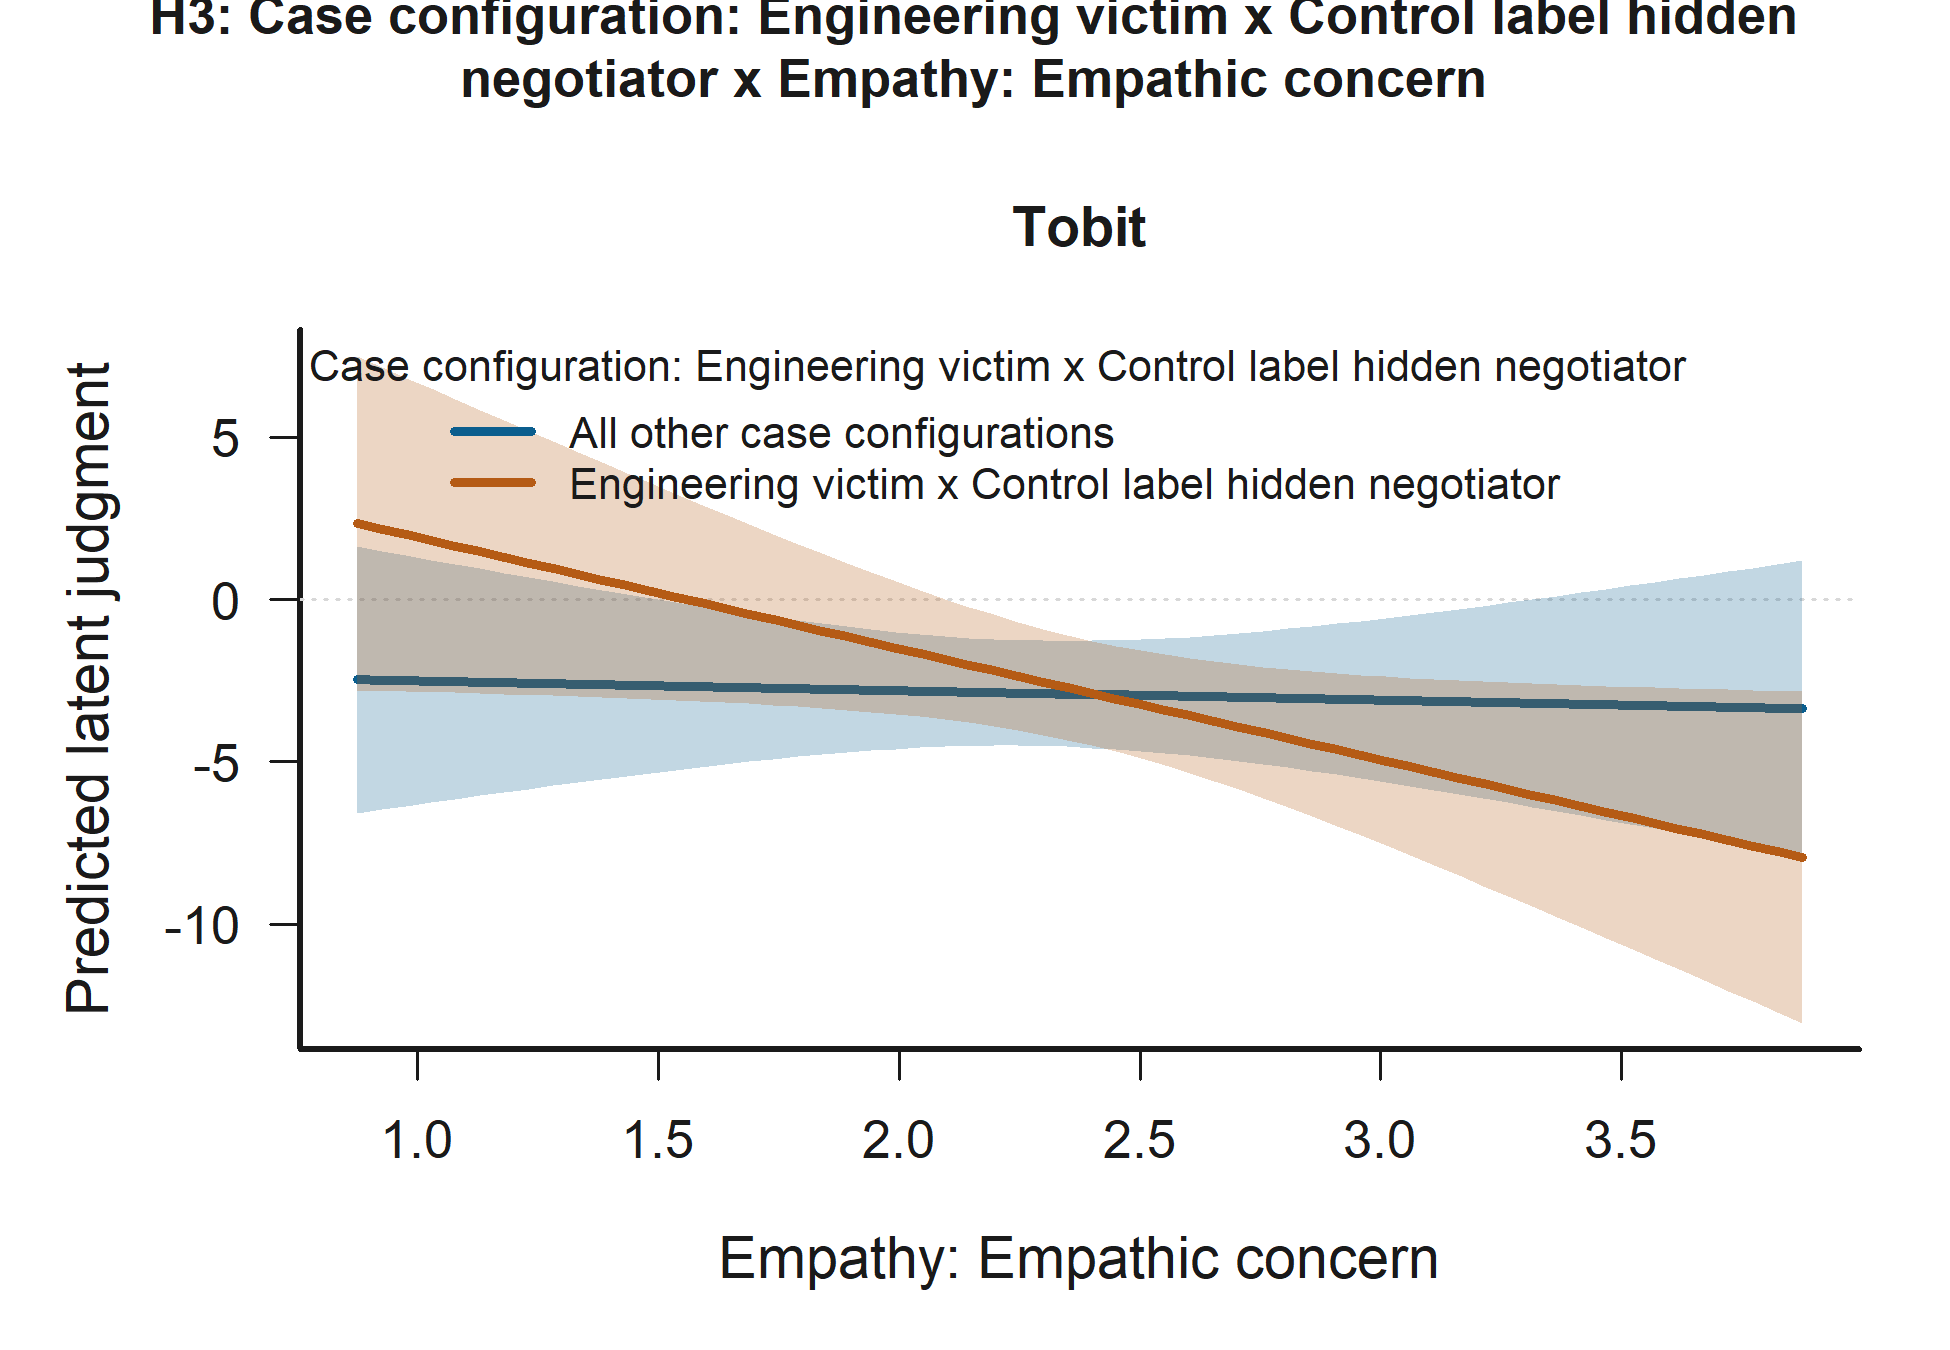
\includegraphics[width=0.92\textwidth]{../figures/figure_sig_H3_case_ing_x_control_iri_ec.png}
\caption{Interaction Plot for Case configuration: Engineering victim x Control label hidden negotiator x Empathy: Empathic concern in H3: Empathy x case-configuration moderation. Support comes from the Tobit model (+, p = 0.055). The panels show predicted latent judgments with 95\% confidence intervals.}
\label{fig:sig_H3_case_ing_x_control_iri_ec}
\end{figure}

Case configuration: Engineering victim x Humanities negotiator x Empathy composite (average) is statistically significant in the Tobit model (+, p = 0.080). Figure \ref{fig:sig_H3_case_ing_x_hum_iri_total} shows that the predicted relationship falls most sharply for Empathy composite (average) when the condition is Engineering victim x Humanities negotiator.

\begin{figure}[H]
\centering
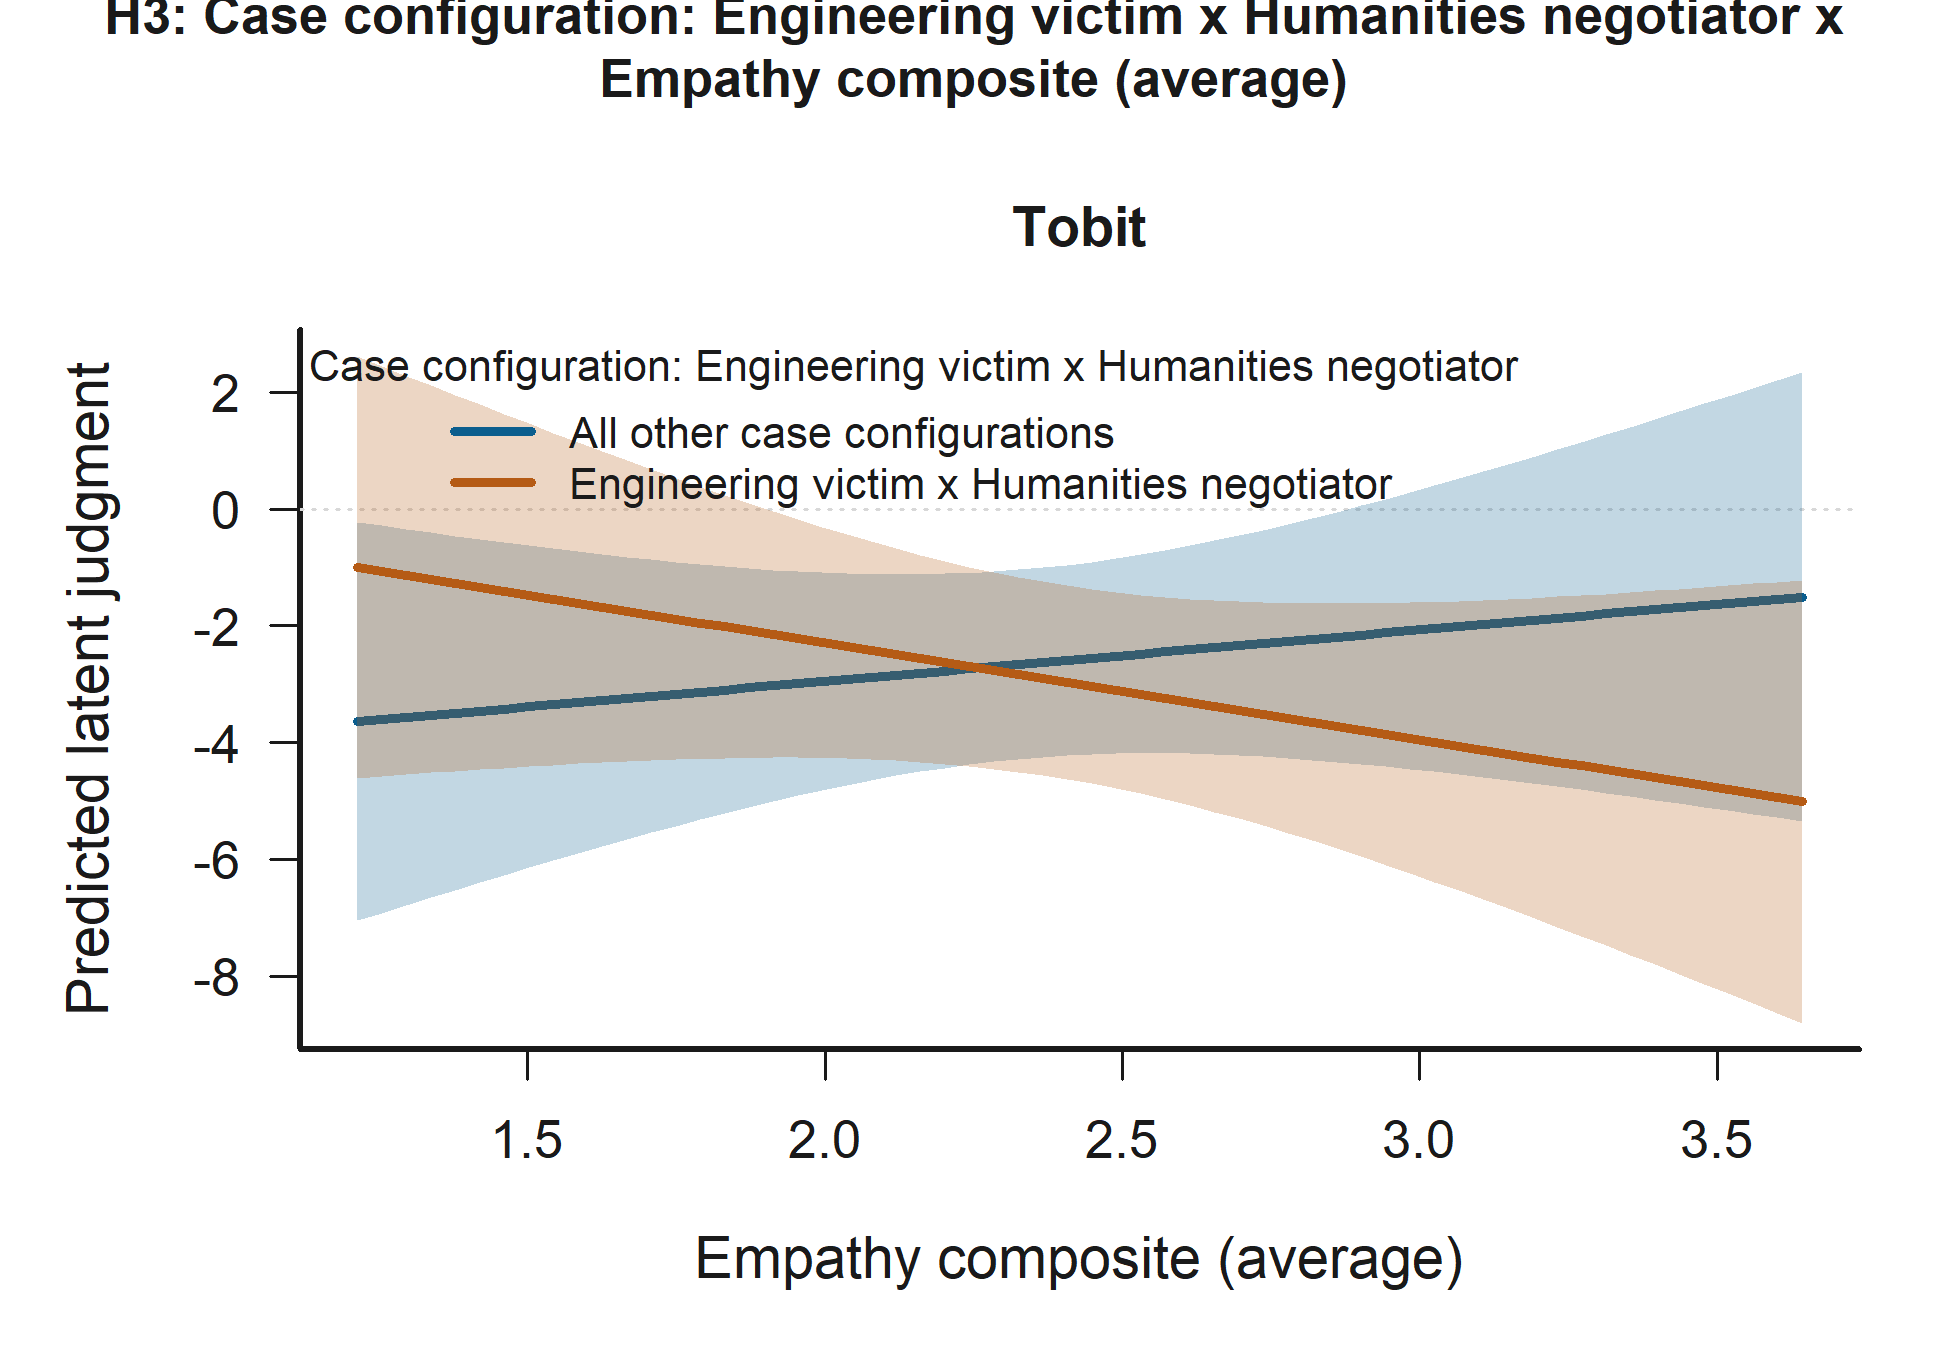
\includegraphics[width=0.92\textwidth]{../figures/figure_sig_H3_case_ing_x_hum_iri_total.png}
\caption{Interaction Plot for Case configuration: Engineering victim x Humanities negotiator x Empathy composite (average) in H3: Empathy x case-configuration moderation. Support comes from the Tobit model (+, p = 0.080). The panels show predicted latent judgments with 95\% confidence intervals.}
\label{fig:sig_H3_case_ing_x_hum_iri_total}
\end{figure}


\subsection{All Significant Predictors (p < 0.10)}
The following figures extend beyond the hypothesis-target terms and visualize every predictor that reaches p < 0.10 in the available H1-H3 Tobit or clustered non-parametric models. This includes significant controls such as age when they clear the threshold.

\paragraph{Accepted-decision sample}

Case configuration: Engineering victim x Humanities negotiator x Empathy: Empathic concern is statistically significant in H3: Empathy x case-configuration moderation Model B (Tobit). Figure \textbackslash\{\}ref\{fig:sig\_all\_accepted\_decision\_sample\_case\_ing\_x\_hum\_iri\_ec\} shows that the predicted relationship falls most sharply for Empathy: Empathic concern when the condition is Engineering victim x Humanities negotiator.

\begin{figure}[H]
\centering
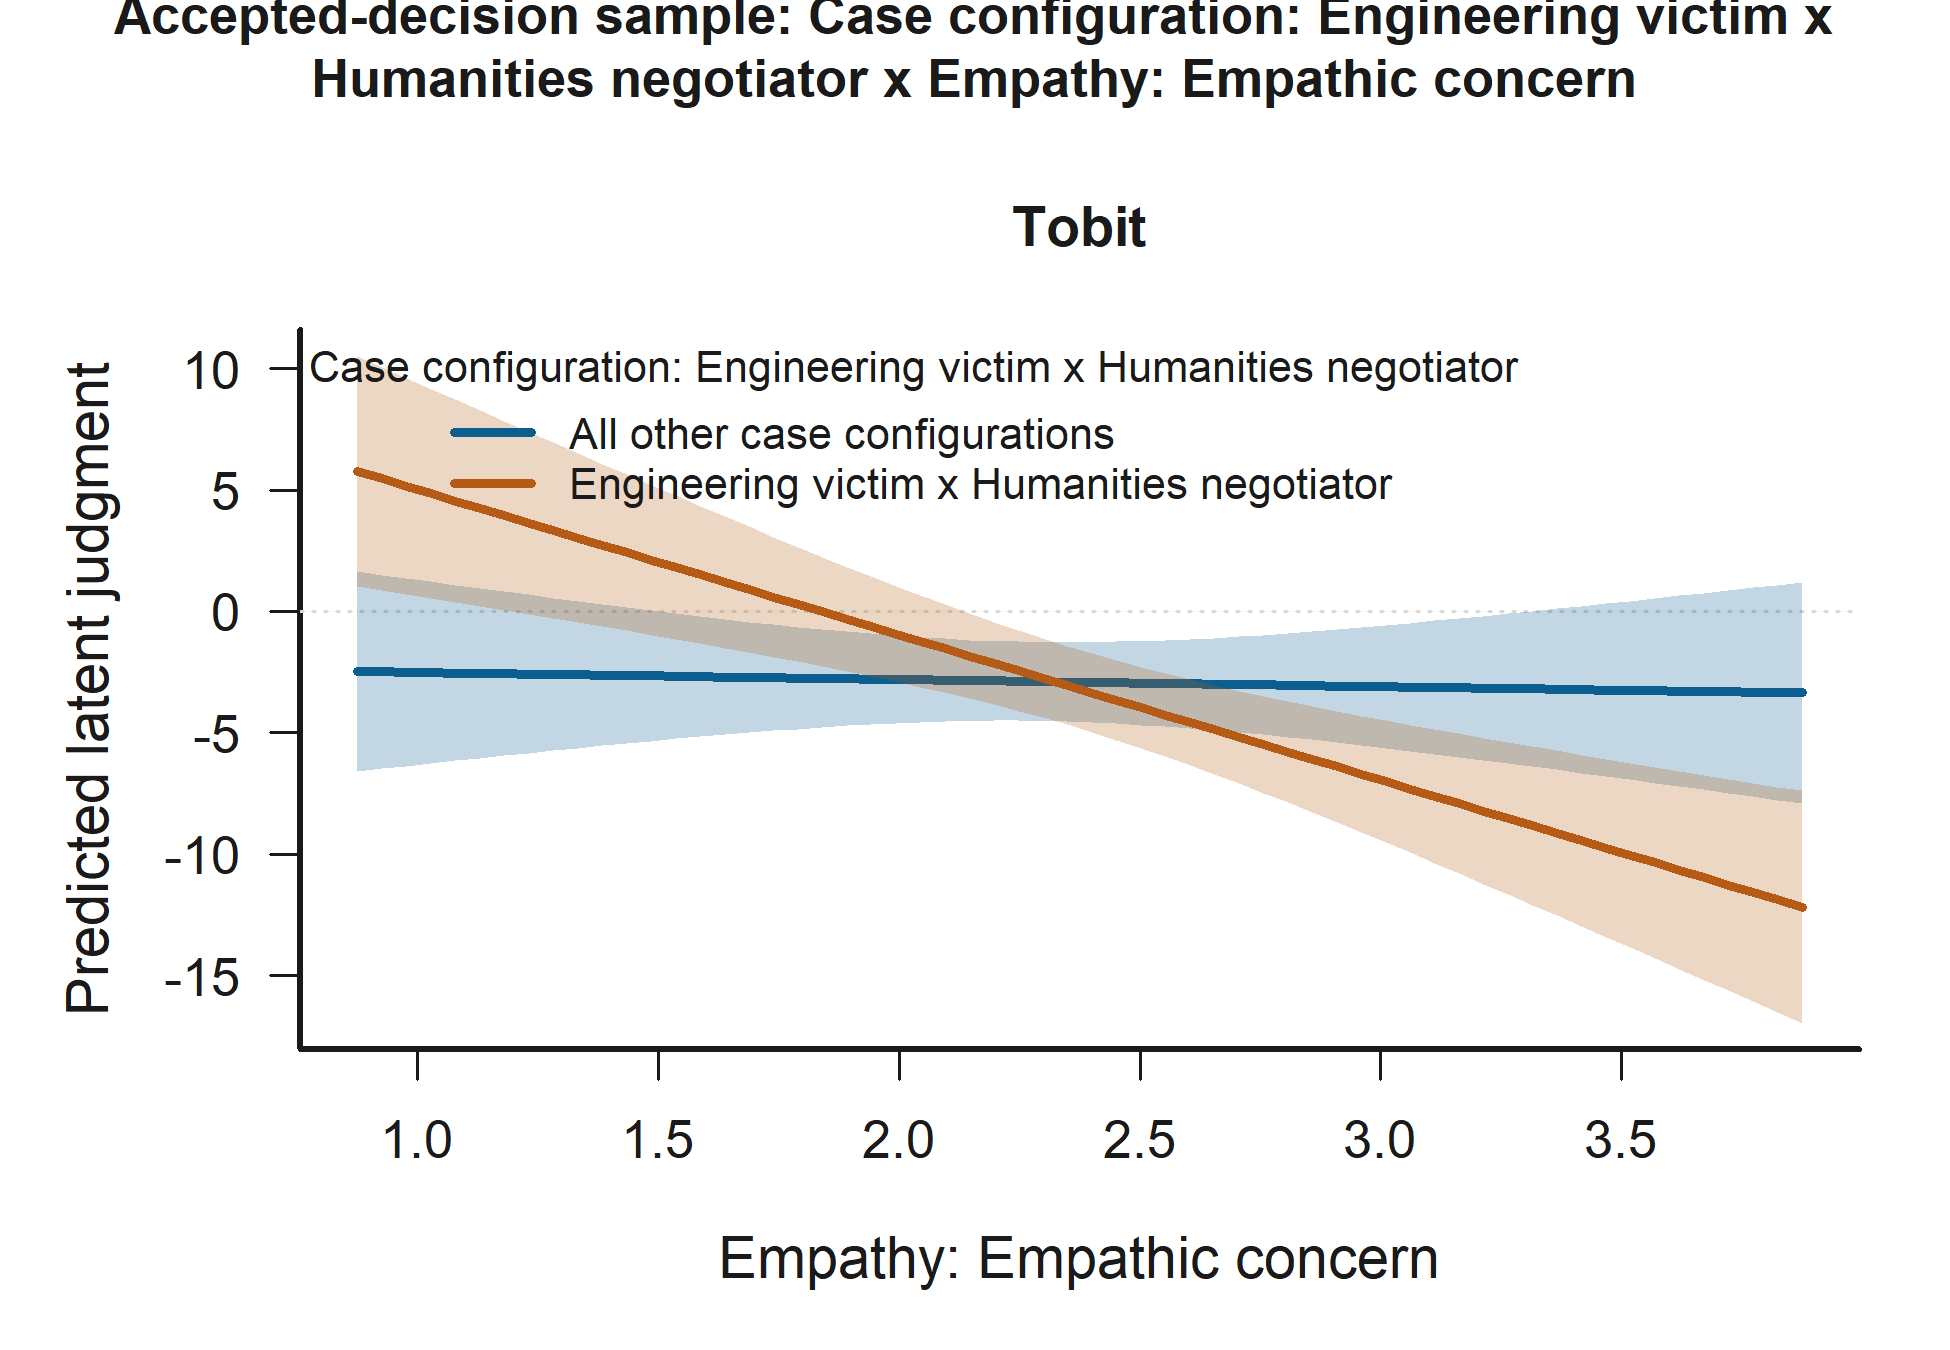
\includegraphics[width=0.92\textwidth]{../figures/figure_sig_all_accepted_decision_sample_case_ing_x_hum_iri_ec.png}
\caption{Interaction Plot for Case configuration: Engineering victim x Humanities negotiator x Empathy: Empathic concern in the Accepted-decision sample. Statistically significant support appears in H3: Empathy x case-configuration moderation Model B (Tobit). The panels show predicted latent judgments with 95\% confidence intervals.}
\label{fig:sig_all_accepted_decision_sample_case_ing_x_hum_iri_ec}
\end{figure}

Observer role (ref = victim) is statistically significant in H2b: Explicit case-configuration contrasts Model A (Tobit), H1: Empathy under explicit case configuration Model A (Tobit), H3: Empathy x case-configuration moderation Model A (Tobit), H2b: Explicit case-configuration contrasts Model B (Tobit), H1: Empathy under explicit case configuration Model B (Tobit), and H3: Empathy x case-configuration moderation Model B (Tobit). Figure \textbackslash\{\}ref\{fig:sig\_all\_accepted\_decision\_sample\_role\_observer\} shows that predicted latent judgment is higher for Observer role than for Victim role.

\begin{figure}[H]
\centering
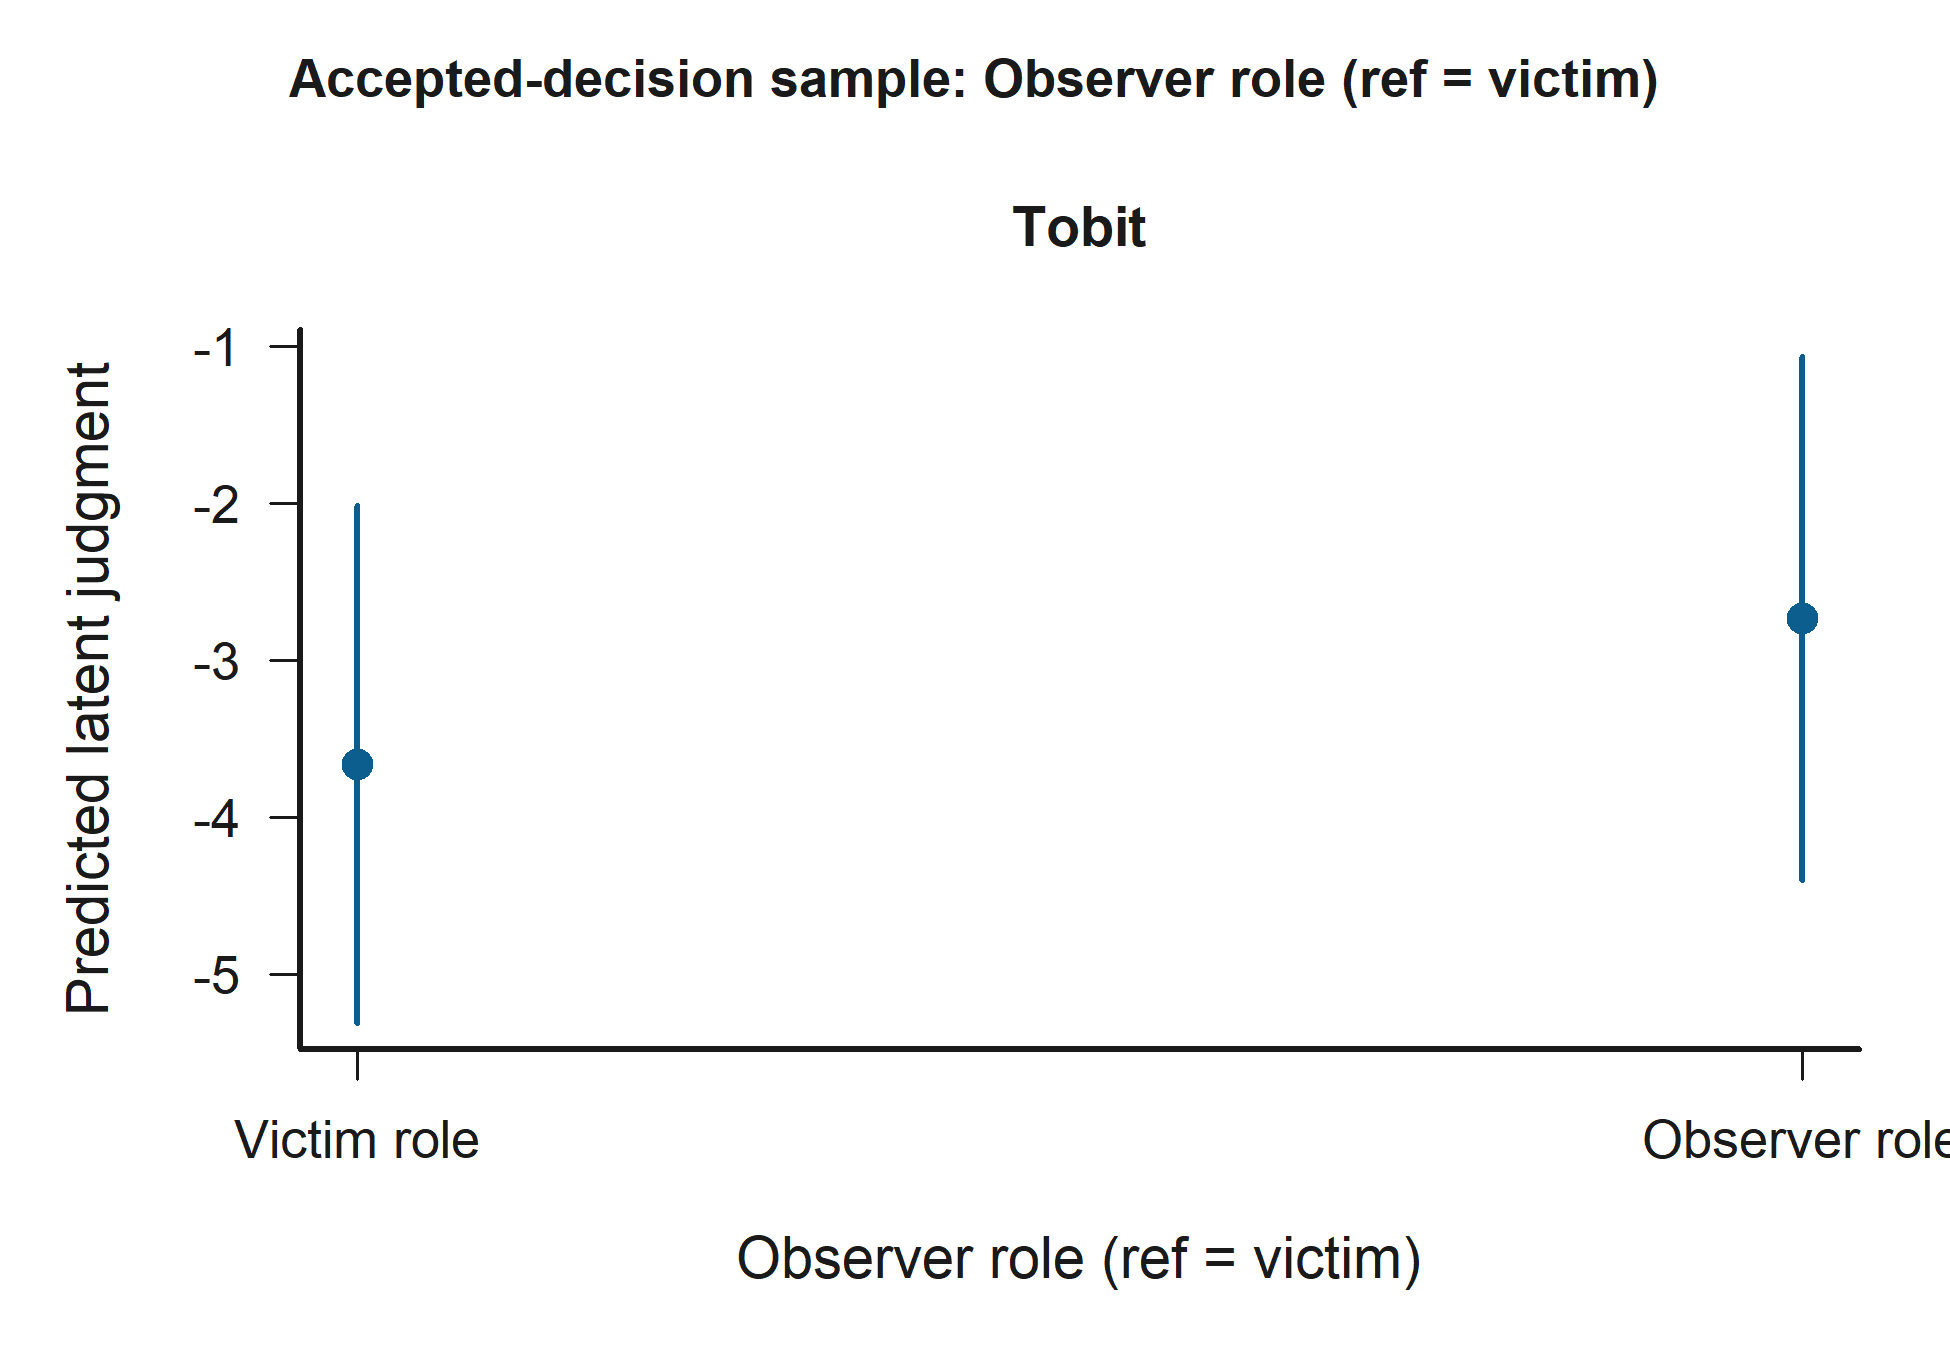
\includegraphics[width=0.92\textwidth]{../figures/figure_sig_all_accepted_decision_sample_role_observer.png}
\caption{Grouped Prediction Plot for Observer role (ref = victim) in the Accepted-decision sample. Statistically significant support appears in H2b: Explicit case-configuration contrasts Model A (Tobit), H1: Empathy under explicit case configuration Model A (Tobit), H3: Empathy x case-configuration moderation Model A (Tobit), H2b: Explicit case-configuration contrasts Model B (Tobit), H1: Empathy under explicit case configuration Model B (Tobit), and H3: Empathy x case-configuration moderation Model B (Tobit). The panels show predicted latent judgments with 95\% confidence intervals.}
\label{fig:sig_all_accepted_decision_sample_role_observer}
\end{figure}

Case configuration: Engineering victim x Humanities negotiator x Empathy: Personal distress is statistically significant in H3: Empathy x case-configuration moderation Model B (Tobit). Figure \textbackslash\{\}ref\{fig:sig\_all\_accepted\_decision\_sample\_case\_ing\_x\_hum\_iri\_pd\} shows that the predicted relationship rises most sharply for Empathy: Personal distress when the condition is Engineering victim x Humanities negotiator.

\begin{figure}[H]
\centering
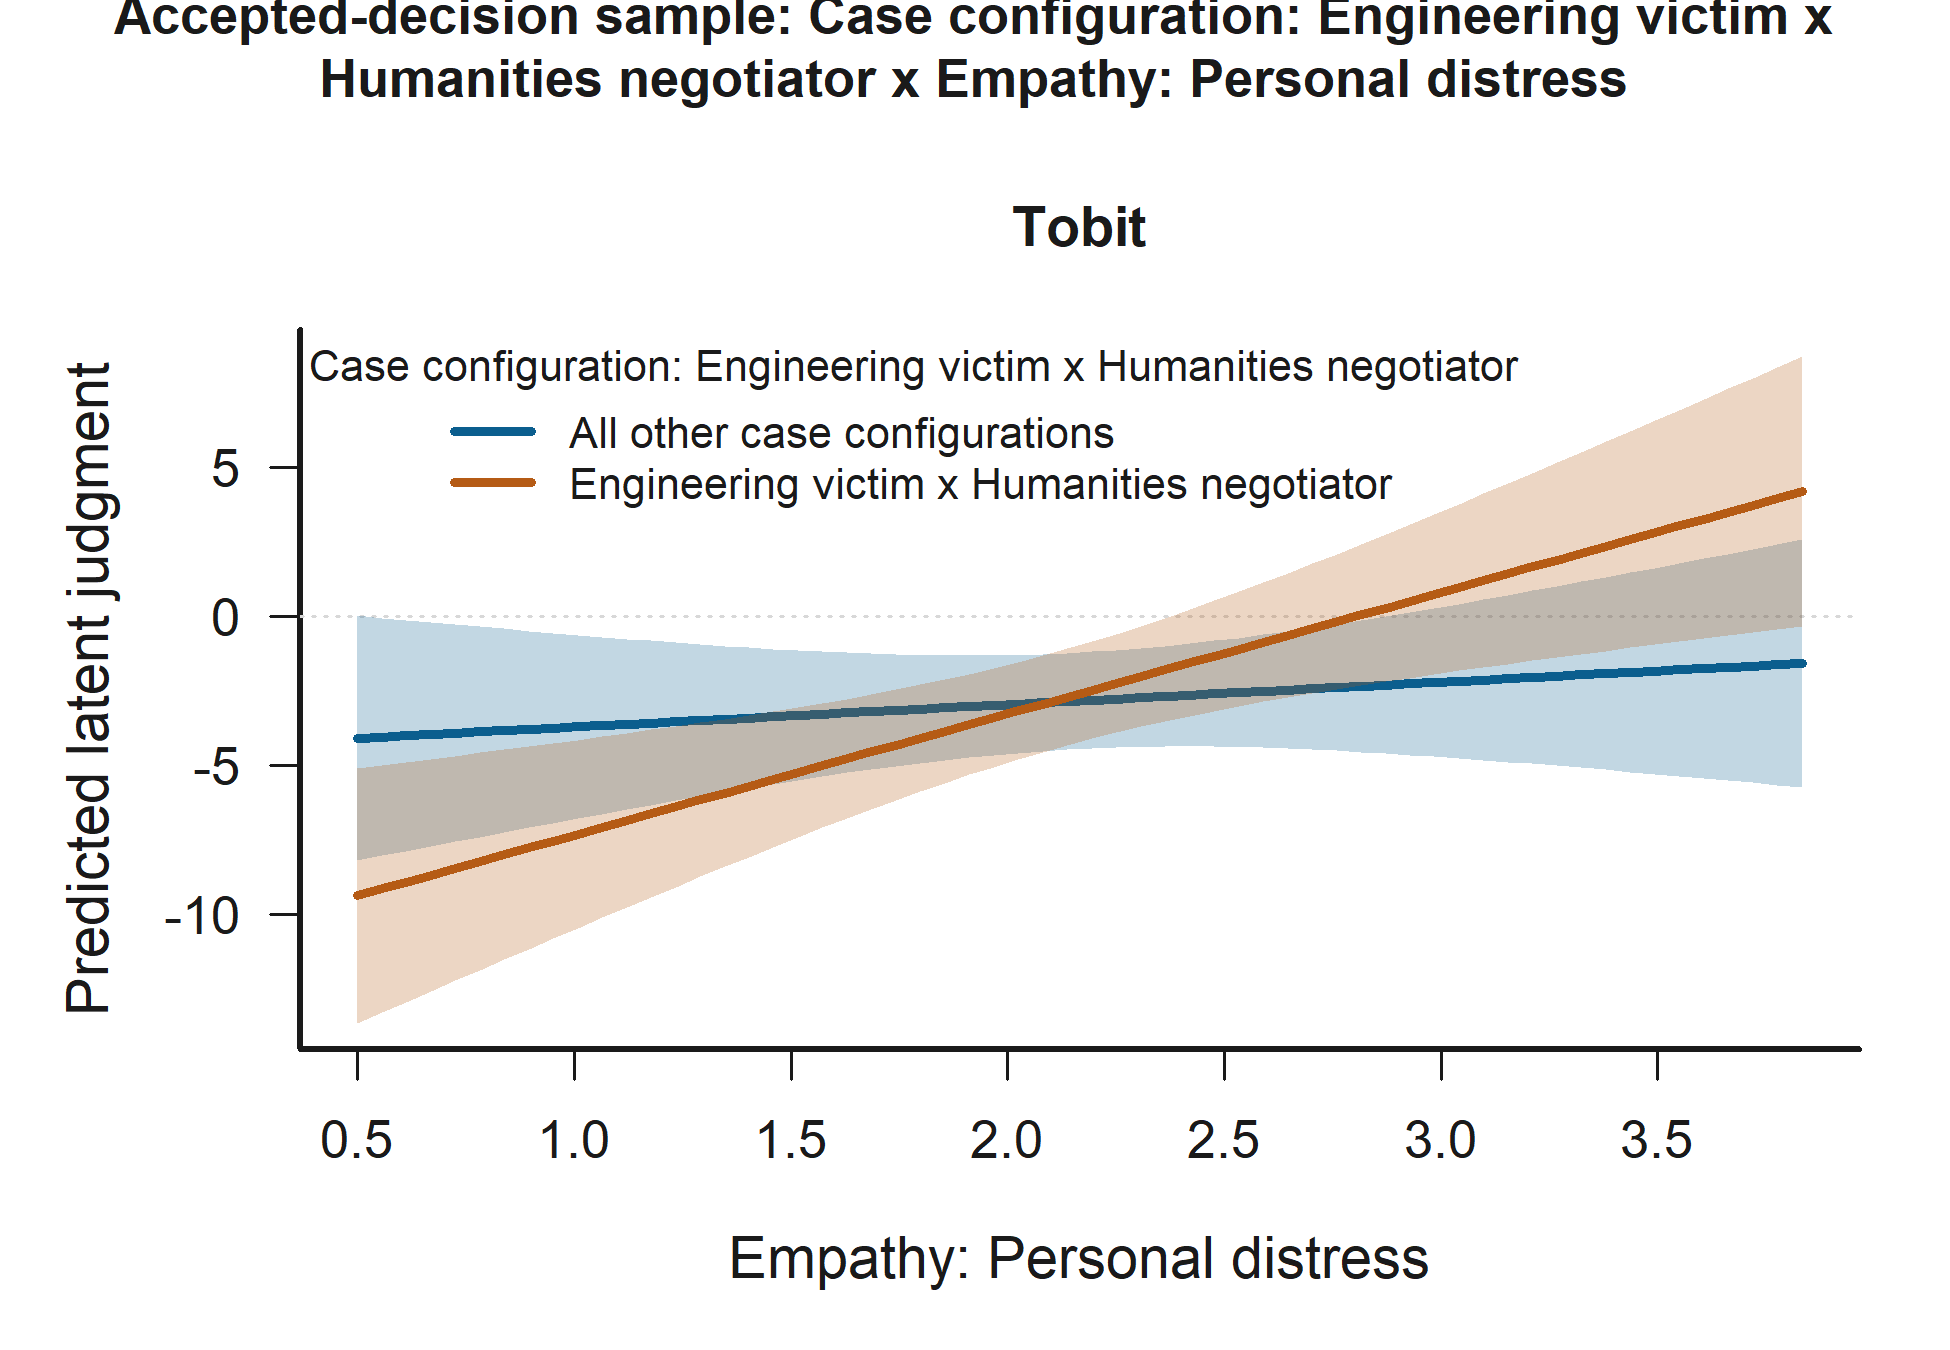
\includegraphics[width=0.92\textwidth]{../figures/figure_sig_all_accepted_decision_sample_case_ing_x_hum_iri_pd.png}
\caption{Interaction Plot for Case configuration: Engineering victim x Humanities negotiator x Empathy: Personal distress in the Accepted-decision sample. Statistically significant support appears in H3: Empathy x case-configuration moderation Model B (Tobit). The panels show predicted latent judgments with 95\% confidence intervals.}
\label{fig:sig_all_accepted_decision_sample_case_ing_x_hum_iri_pd}
\end{figure}

Empathy: Empathic concern is statistically significant in H1: Empathy under explicit case configuration Model B (Tobit) and H2b: Explicit case-configuration contrasts Model B (Tobit). Figure \textbackslash\{\}ref\{fig:sig\_all\_accepted\_decision\_sample\_iri\_ec\} shows that across the observed range, higher Empathy: Empathic concern corresponds to lower predicted latent judgment.

\begin{figure}[H]
\centering
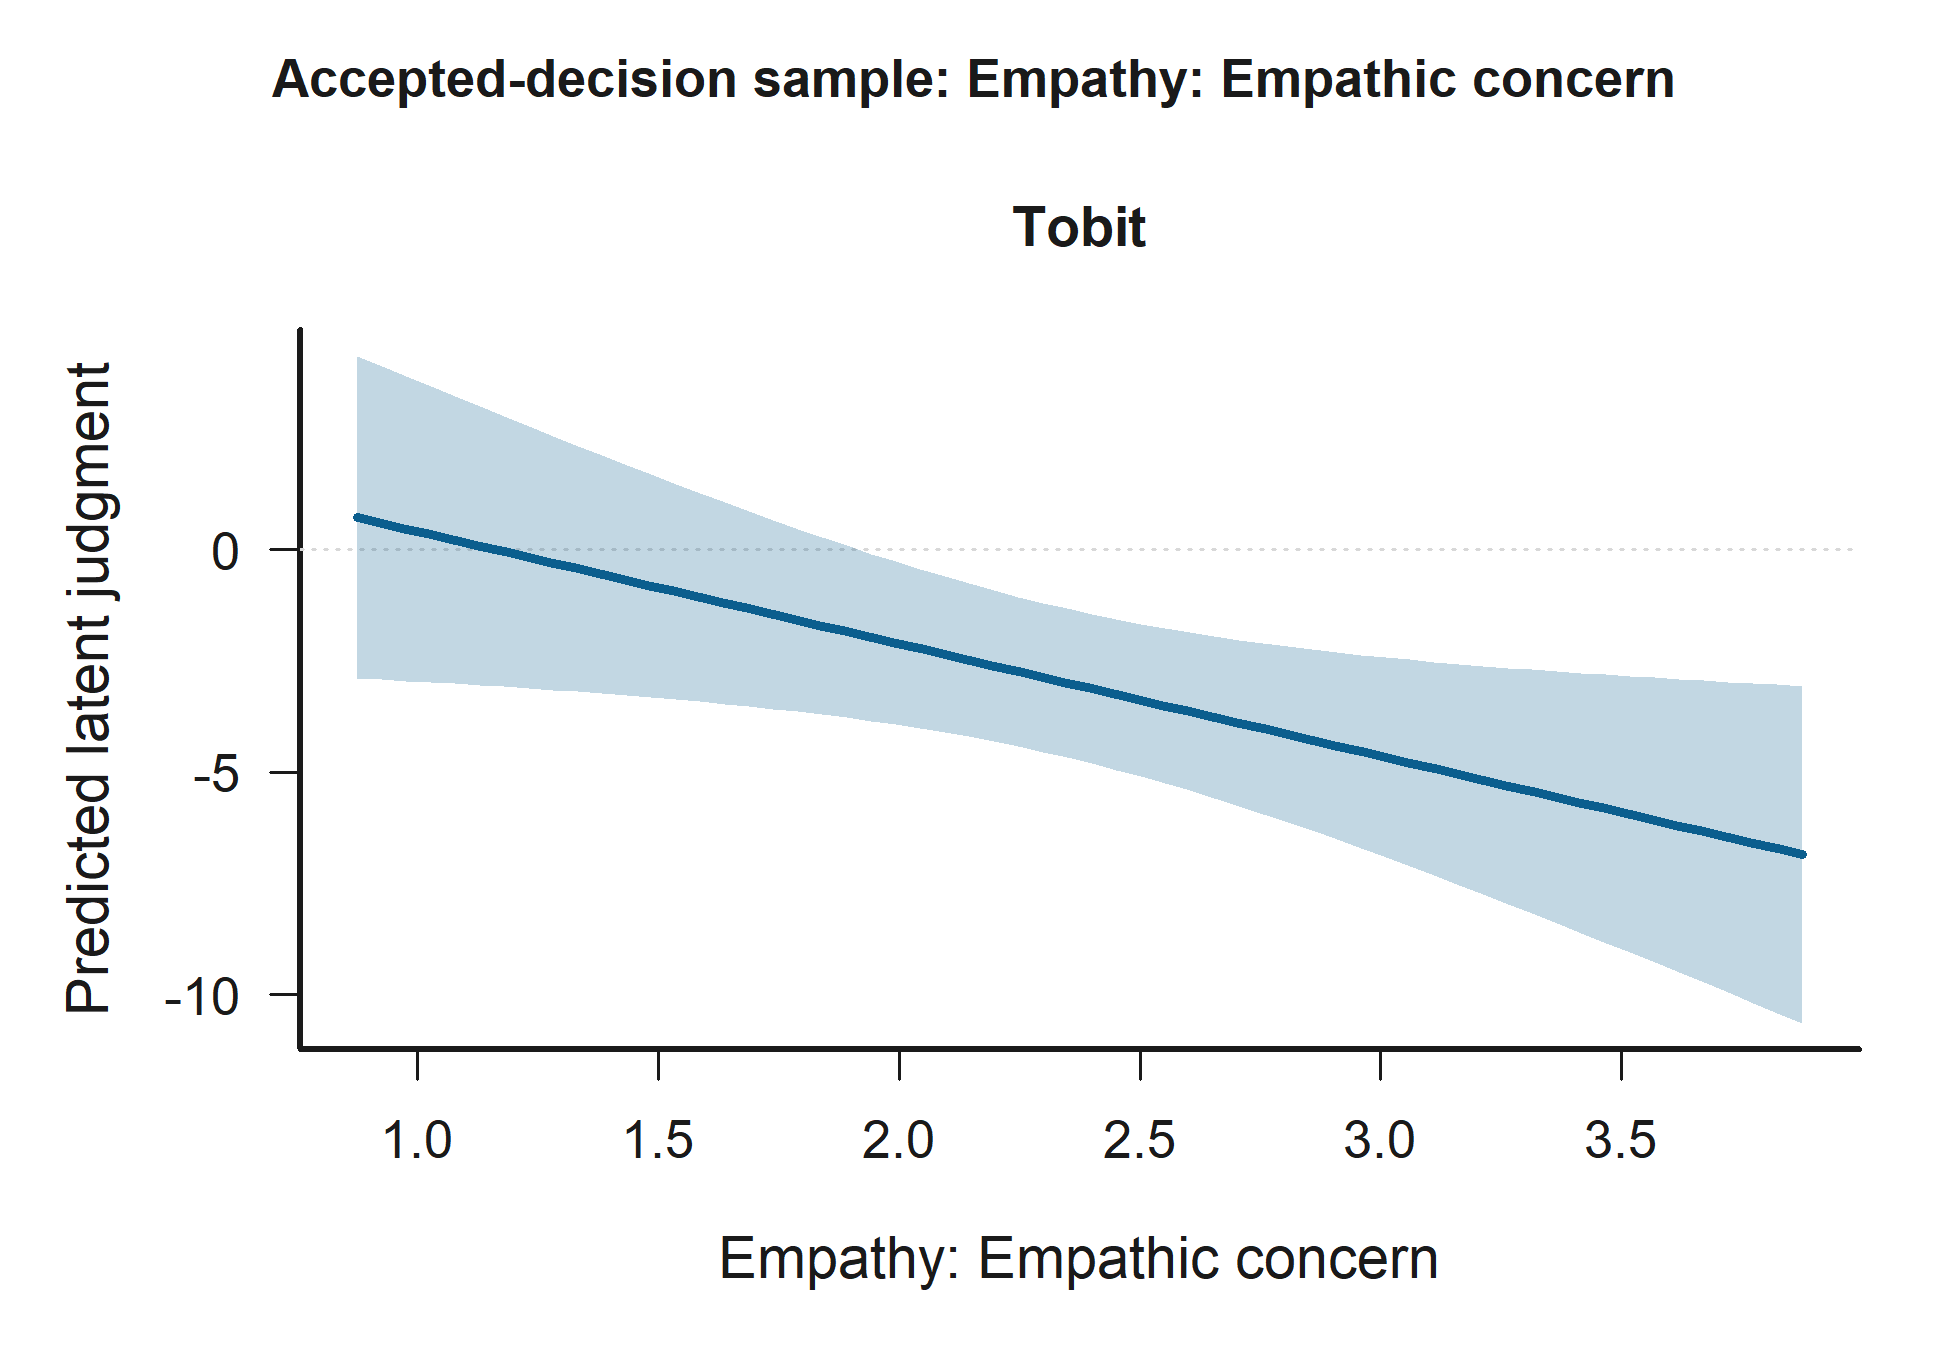
\includegraphics[width=0.92\textwidth]{../figures/figure_sig_all_accepted_decision_sample_iri_ec.png}
\caption{Effect Plot for Empathy: Empathic concern in the Accepted-decision sample. Statistically significant support appears in H1: Empathy under explicit case configuration Model B (Tobit) and H2b: Explicit case-configuration contrasts Model B (Tobit). The panels show predicted latent judgments with 95\% confidence intervals.}
\label{fig:sig_all_accepted_decision_sample_iri_ec}
\end{figure}

Age is statistically significant in H3: Empathy x case-configuration moderation Model A (Tobit), H1: Empathy under explicit case configuration Model A (Tobit), H2b: Explicit case-configuration contrasts Model A (Tobit), H2b: Explicit case-configuration contrasts Model B (Tobit), H1: Empathy under explicit case configuration Model B (Tobit), and H3: Empathy x case-configuration moderation Model B (Tobit). Figure \textbackslash\{\}ref\{fig:sig\_all\_accepted\_decision\_sample\_age\} shows that across the observed range, higher Age corresponds to higher predicted latent judgment.

\begin{figure}[H]
\centering
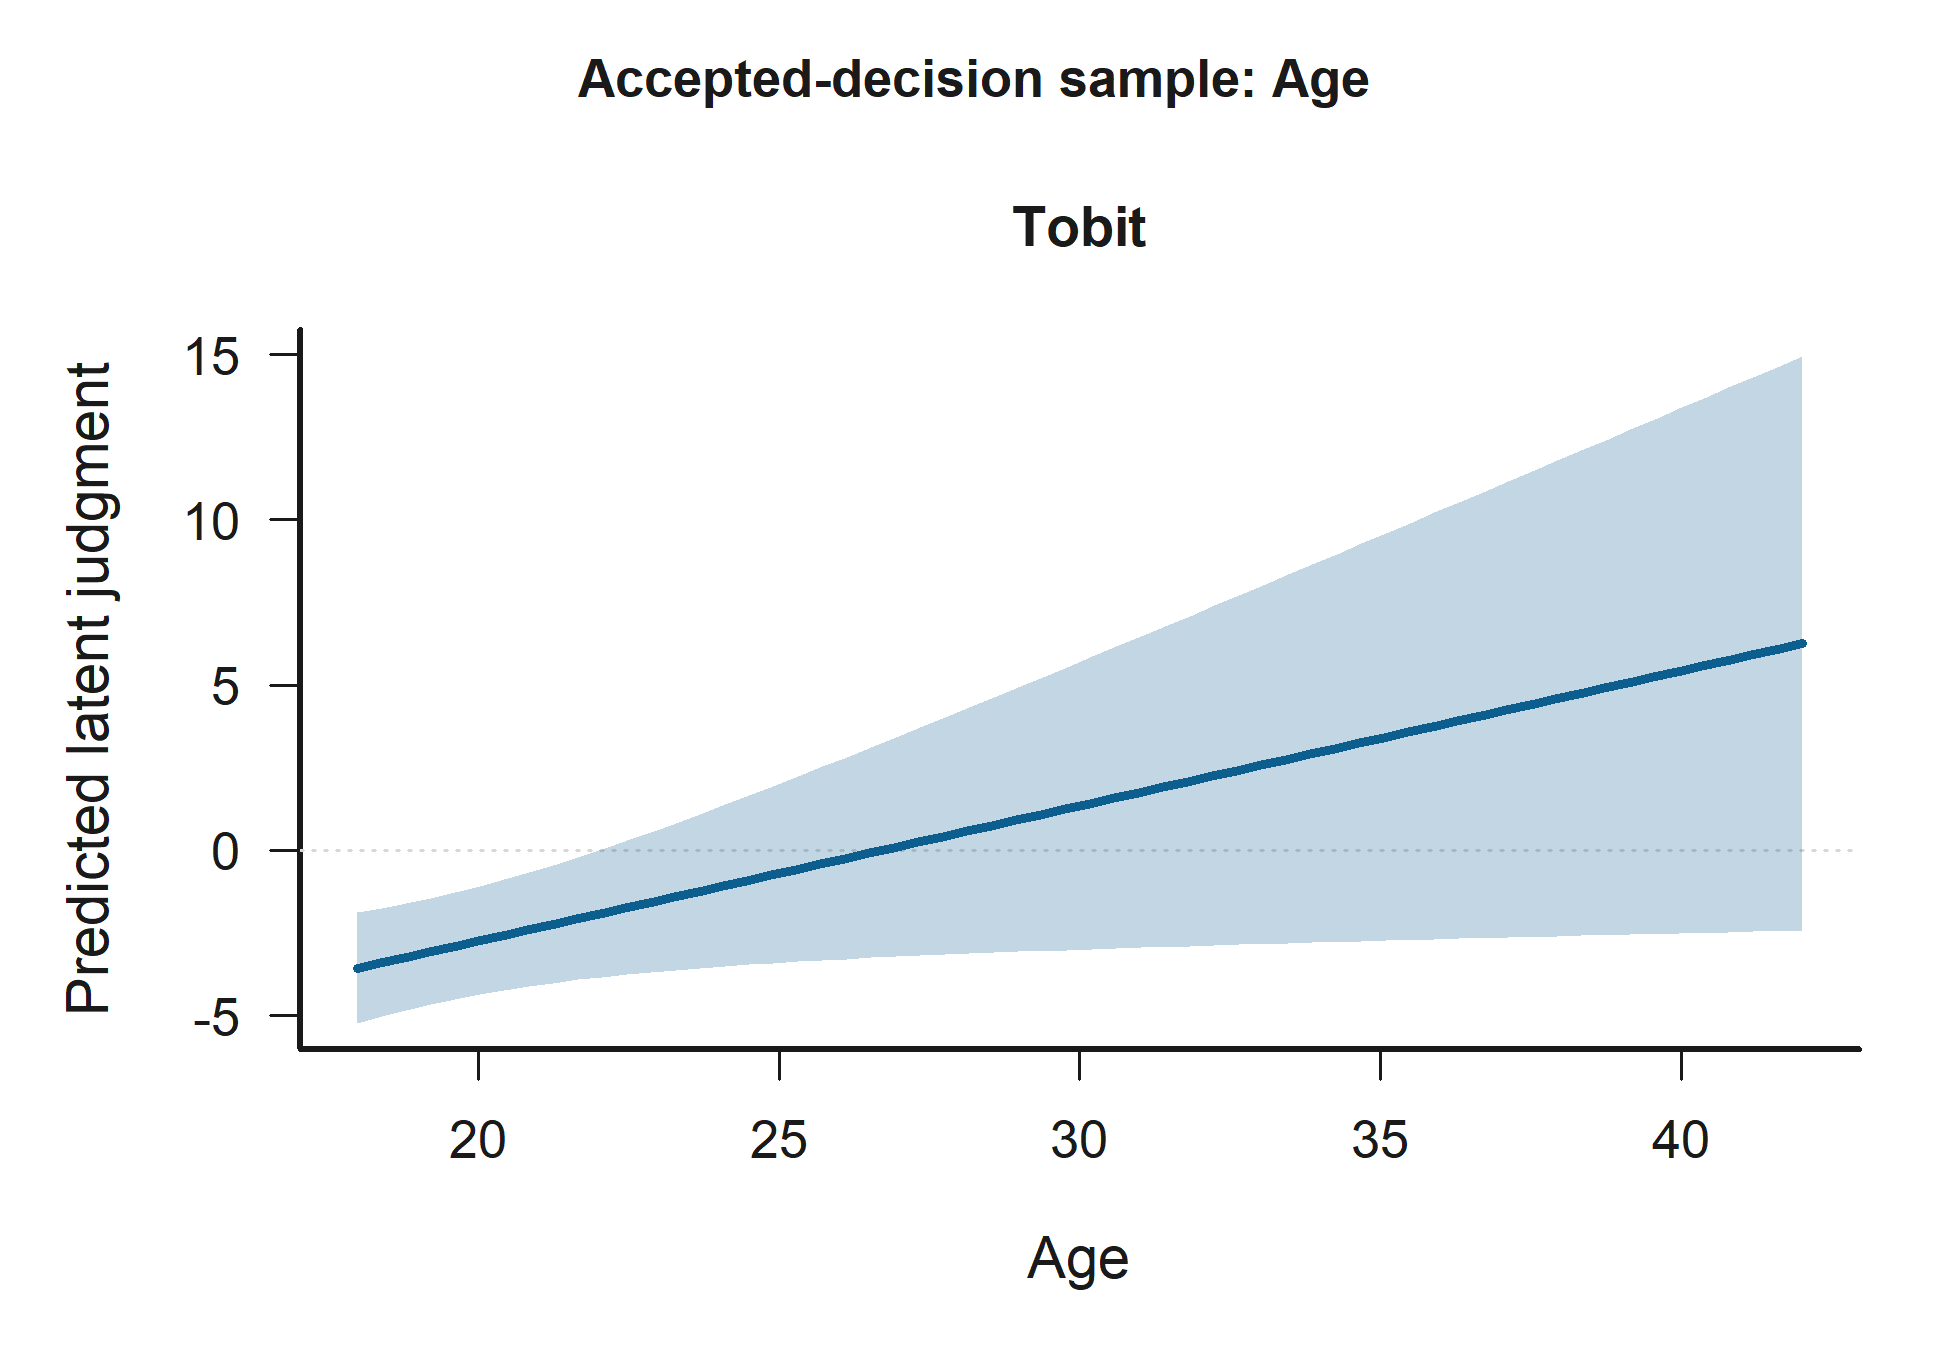
\includegraphics[width=0.92\textwidth]{../figures/figure_sig_all_accepted_decision_sample_age.png}
\caption{Effect Plot for Age in the Accepted-decision sample. Statistically significant support appears in H3: Empathy x case-configuration moderation Model A (Tobit), H1: Empathy under explicit case configuration Model A (Tobit), H2b: Explicit case-configuration contrasts Model A (Tobit), H2b: Explicit case-configuration contrasts Model B (Tobit), H1: Empathy under explicit case configuration Model B (Tobit), and H3: Empathy x case-configuration moderation Model B (Tobit). The panels show predicted latent judgments with 95\% confidence intervals.}
\label{fig:sig_all_accepted_decision_sample_age}
\end{figure}

Empathy: Perspective taking is statistically significant in H2b: Explicit case-configuration contrasts Model B (Tobit) and H1: Empathy under explicit case configuration Model B (Tobit). Figure \textbackslash\{\}ref\{fig:sig\_all\_accepted\_decision\_sample\_iri\_pt\} shows that across the observed range, higher Empathy: Perspective taking corresponds to higher predicted latent judgment.

\begin{figure}[H]
\centering
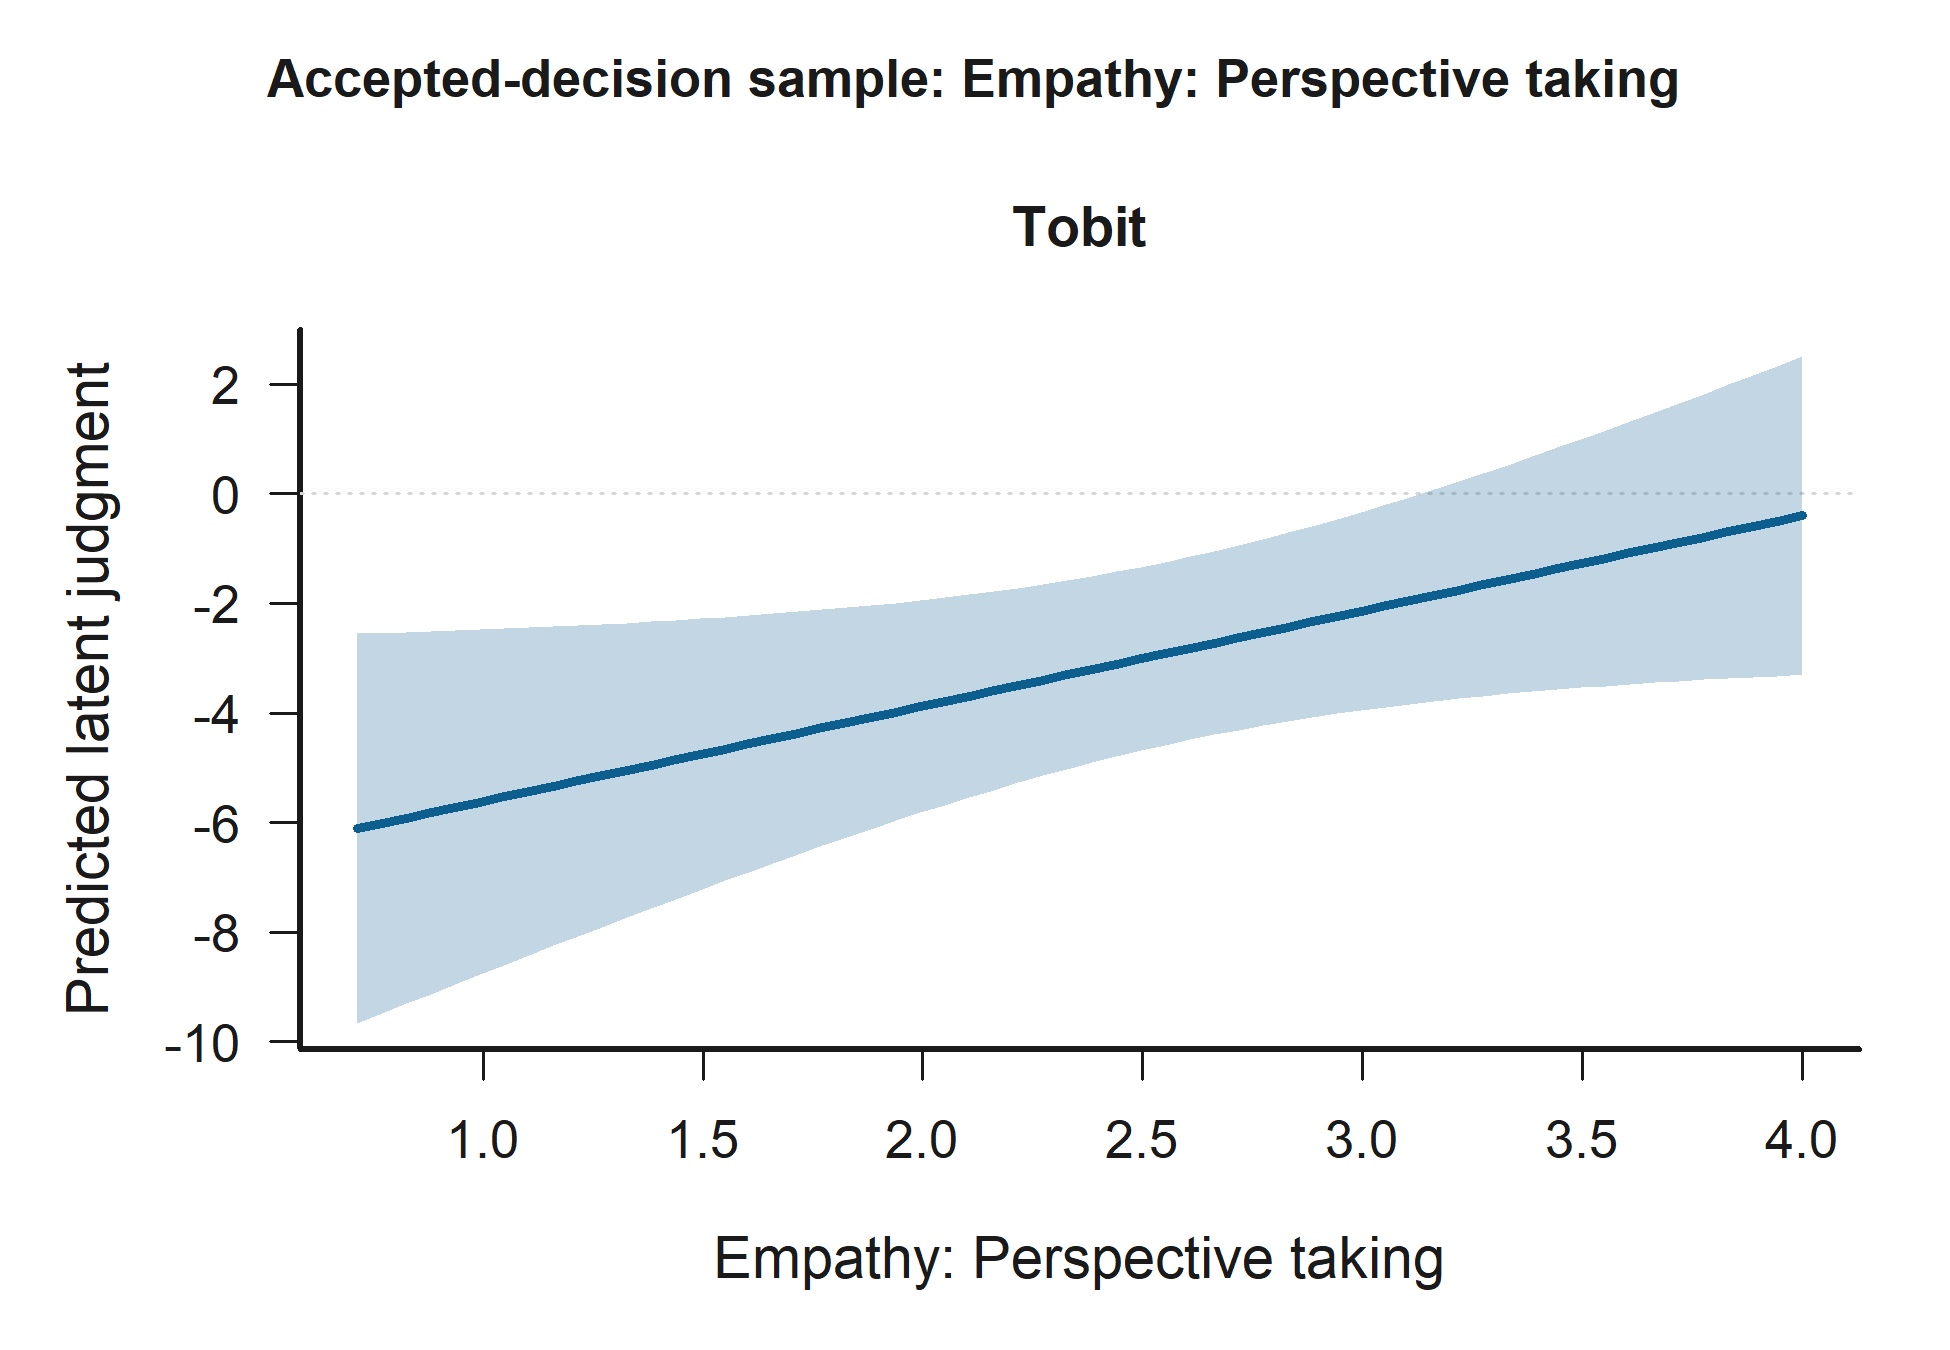
\includegraphics[width=0.92\textwidth]{../figures/figure_sig_all_accepted_decision_sample_iri_pt.png}
\caption{Effect Plot for Empathy: Perspective taking in the Accepted-decision sample. Statistically significant support appears in H2b: Explicit case-configuration contrasts Model B (Tobit) and H1: Empathy under explicit case configuration Model B (Tobit). The panels show predicted latent judgments with 95\% confidence intervals.}
\label{fig:sig_all_accepted_decision_sample_iri_pt}
\end{figure}

Case configuration: Humanities victim x Engineering negotiator x Empathy composite (average) is statistically significant in H3: Empathy x case-configuration moderation Model A (Tobit). Figure \textbackslash\{\}ref\{fig:sig\_all\_accepted\_decision\_sample\_case\_hum\_x\_ing\_iri\_total\} shows that the predicted relationship falls most sharply for Empathy composite (average) when the condition is Humanities victim x Engineering negotiator.

\begin{figure}[H]
\centering
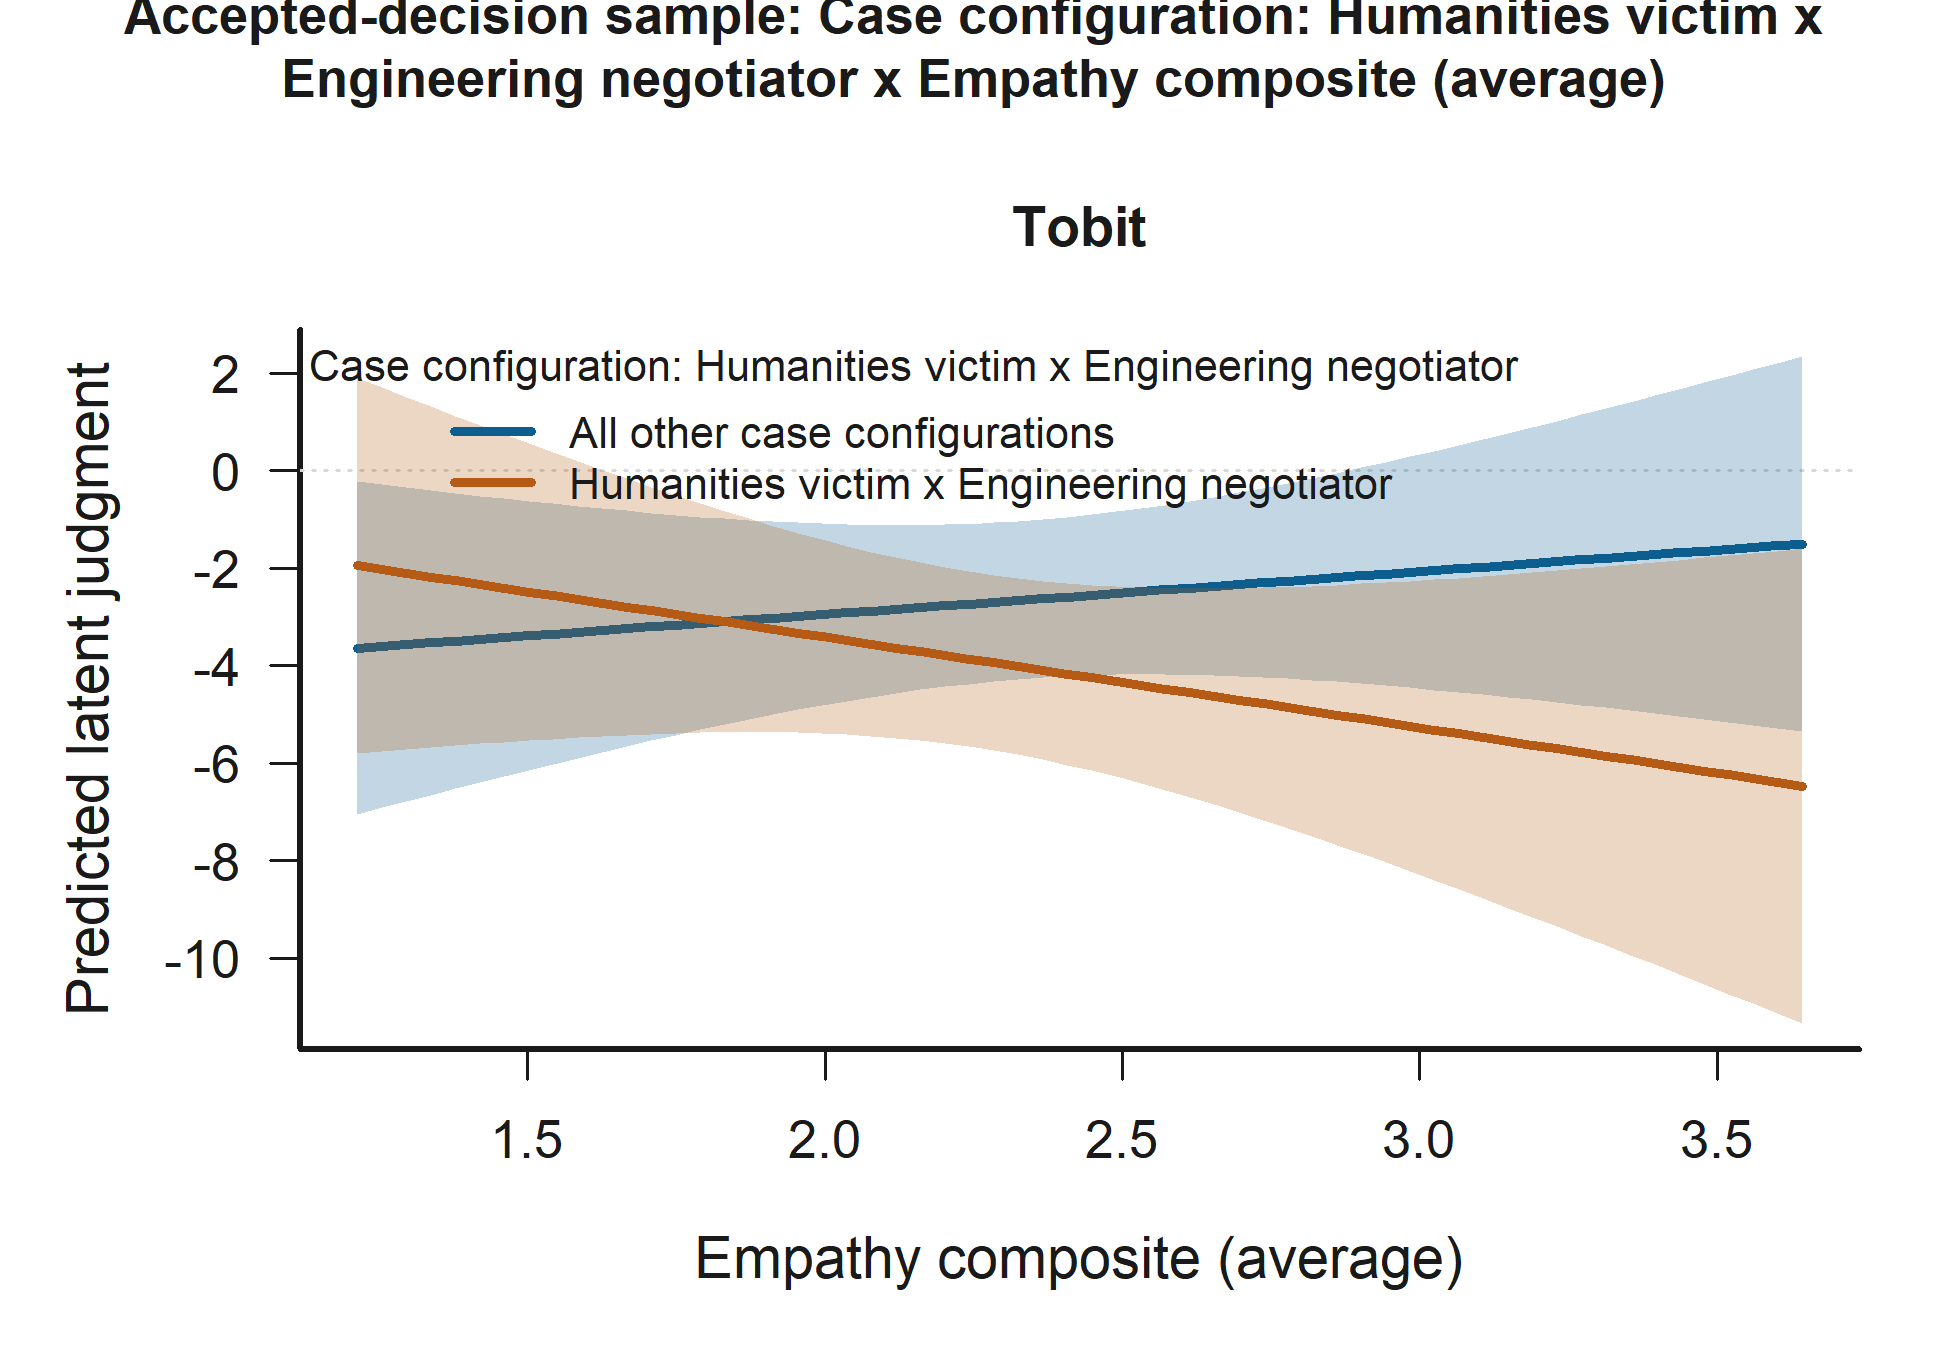
\includegraphics[width=0.92\textwidth]{../figures/figure_sig_all_accepted_decision_sample_case_hum_x_ing_iri_total.png}
\caption{Interaction Plot for Case configuration: Humanities victim x Engineering negotiator x Empathy composite (average) in the Accepted-decision sample. Statistically significant support appears in H3: Empathy x case-configuration moderation Model A (Tobit). The panels show predicted latent judgments with 95\% confidence intervals.}
\label{fig:sig_all_accepted_decision_sample_case_hum_x_ing_iri_total}
\end{figure}

Case configuration: Engineering victim x Control label hidden negotiator x Empathy: Empathic concern is statistically significant in H3: Empathy x case-configuration moderation Model B (Tobit). Figure \textbackslash\{\}ref\{fig:sig\_all\_accepted\_decision\_sample\_case\_ing\_x\_control\_iri\_ec\} shows that the predicted relationship falls most sharply for Empathy: Empathic concern when the condition is Engineering victim x Control label hidden negotiator.

\begin{figure}[H]
\centering
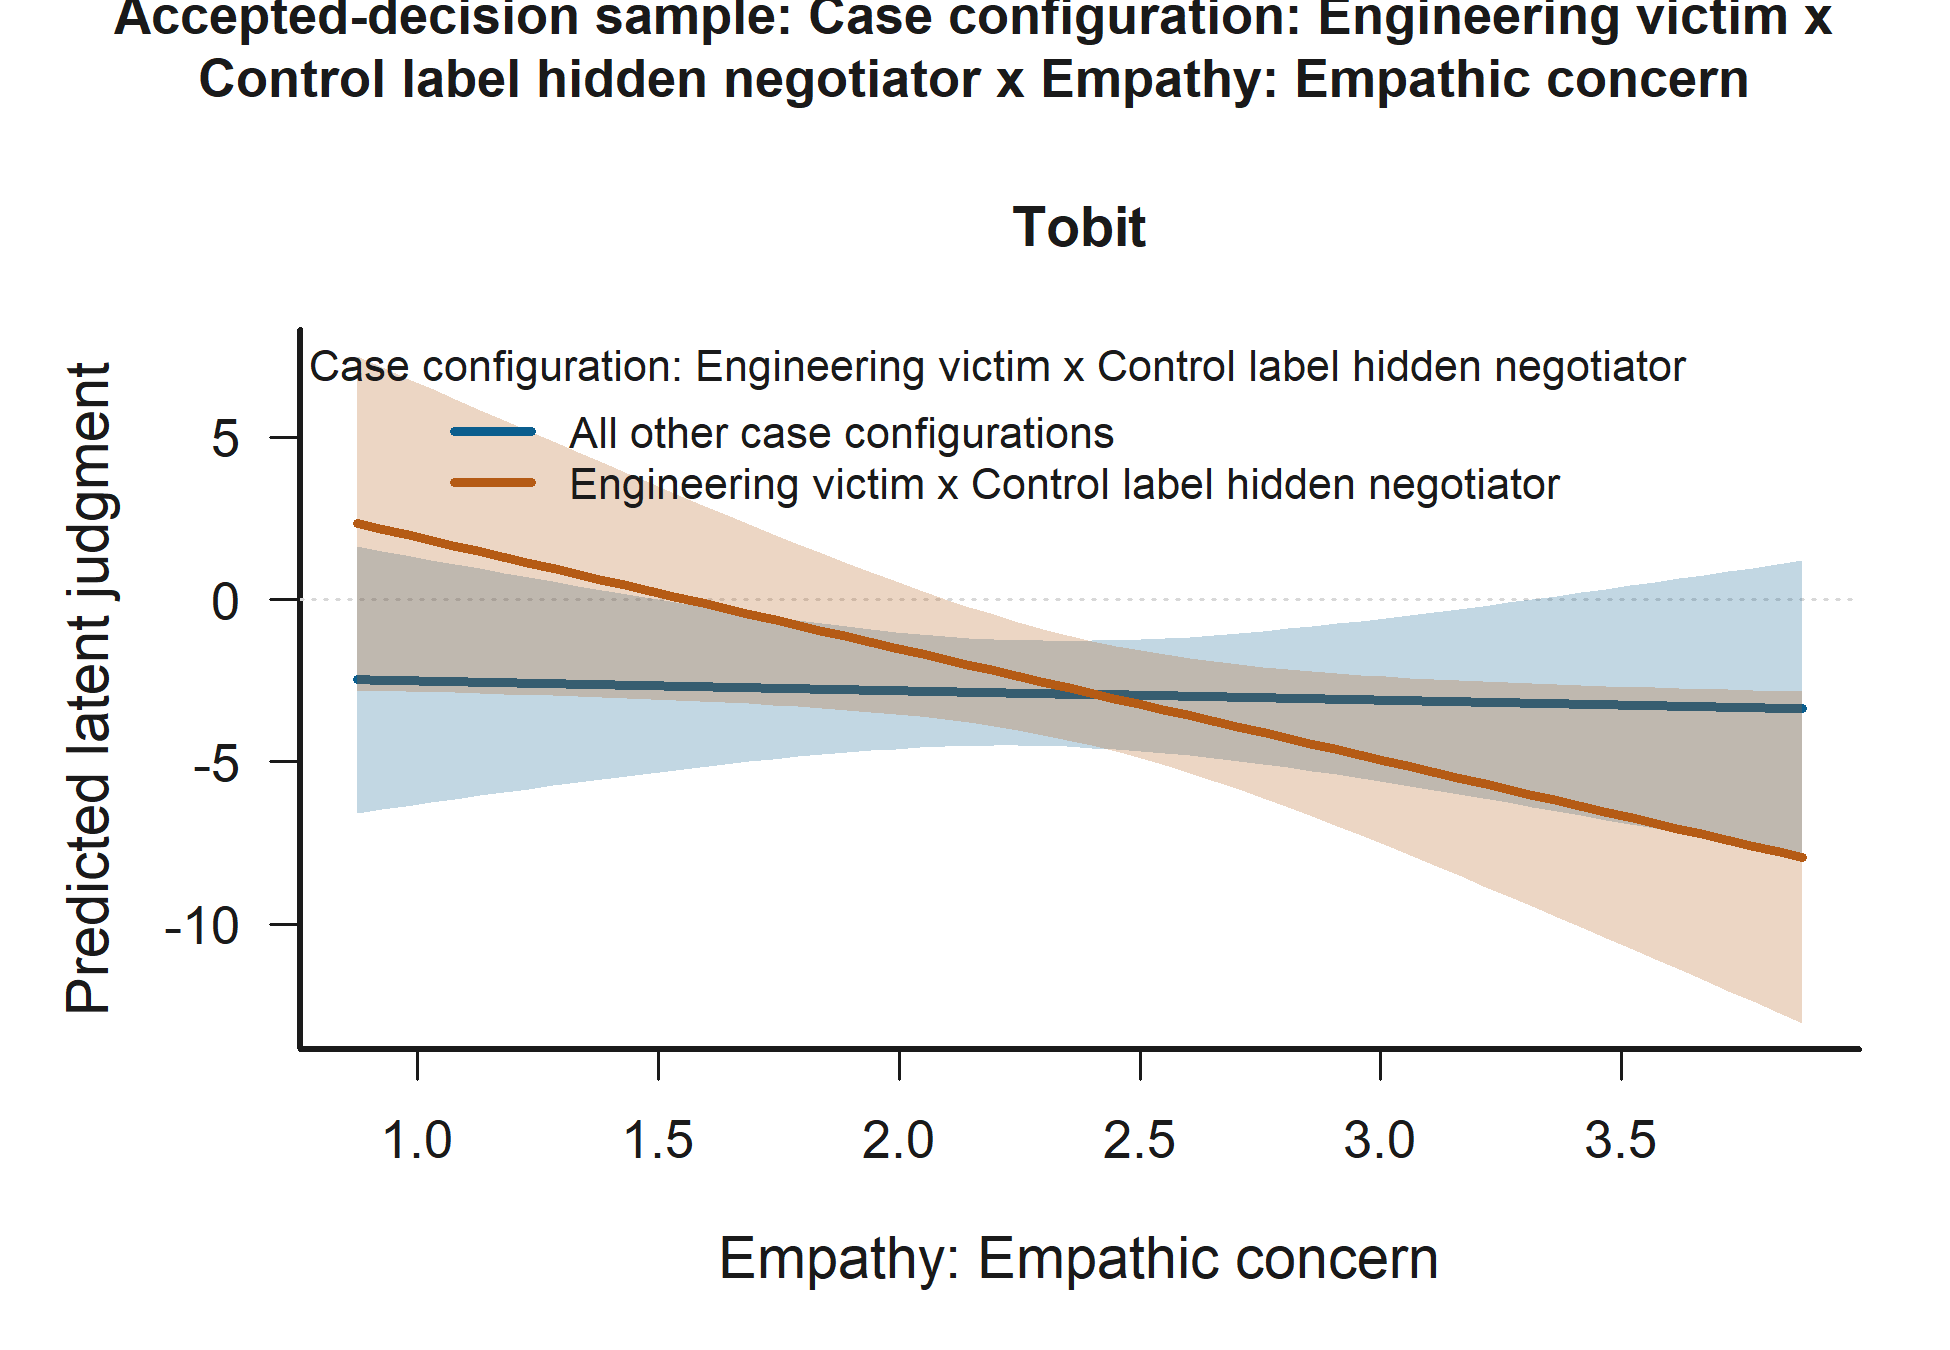
\includegraphics[width=0.92\textwidth]{../figures/figure_sig_all_accepted_decision_sample_case_ing_x_control_iri_ec.png}
\caption{Interaction Plot for Case configuration: Engineering victim x Control label hidden negotiator x Empathy: Empathic concern in the Accepted-decision sample. Statistically significant support appears in H3: Empathy x case-configuration moderation Model B (Tobit). The panels show predicted latent judgments with 95\% confidence intervals.}
\label{fig:sig_all_accepted_decision_sample_case_ing_x_control_iri_ec}
\end{figure}

Case configuration: Humanities victim x Engineering negotiator is statistically significant in H1: Empathy under explicit case configuration Model A (Tobit), H2b: Explicit case-configuration contrasts Model A (Tobit), H1: Empathy under explicit case configuration Model B (Tobit), and H2b: Explicit case-configuration contrasts Model B (Tobit). Figure \textbackslash\{\}ref\{fig:sig\_all\_accepted\_decision\_sample\_case\_hum\_x\_ing\} shows that predicted latent judgment is lower for Humanities victim x Engineering negotiator than for All other case configurations.

\begin{figure}[H]
\centering
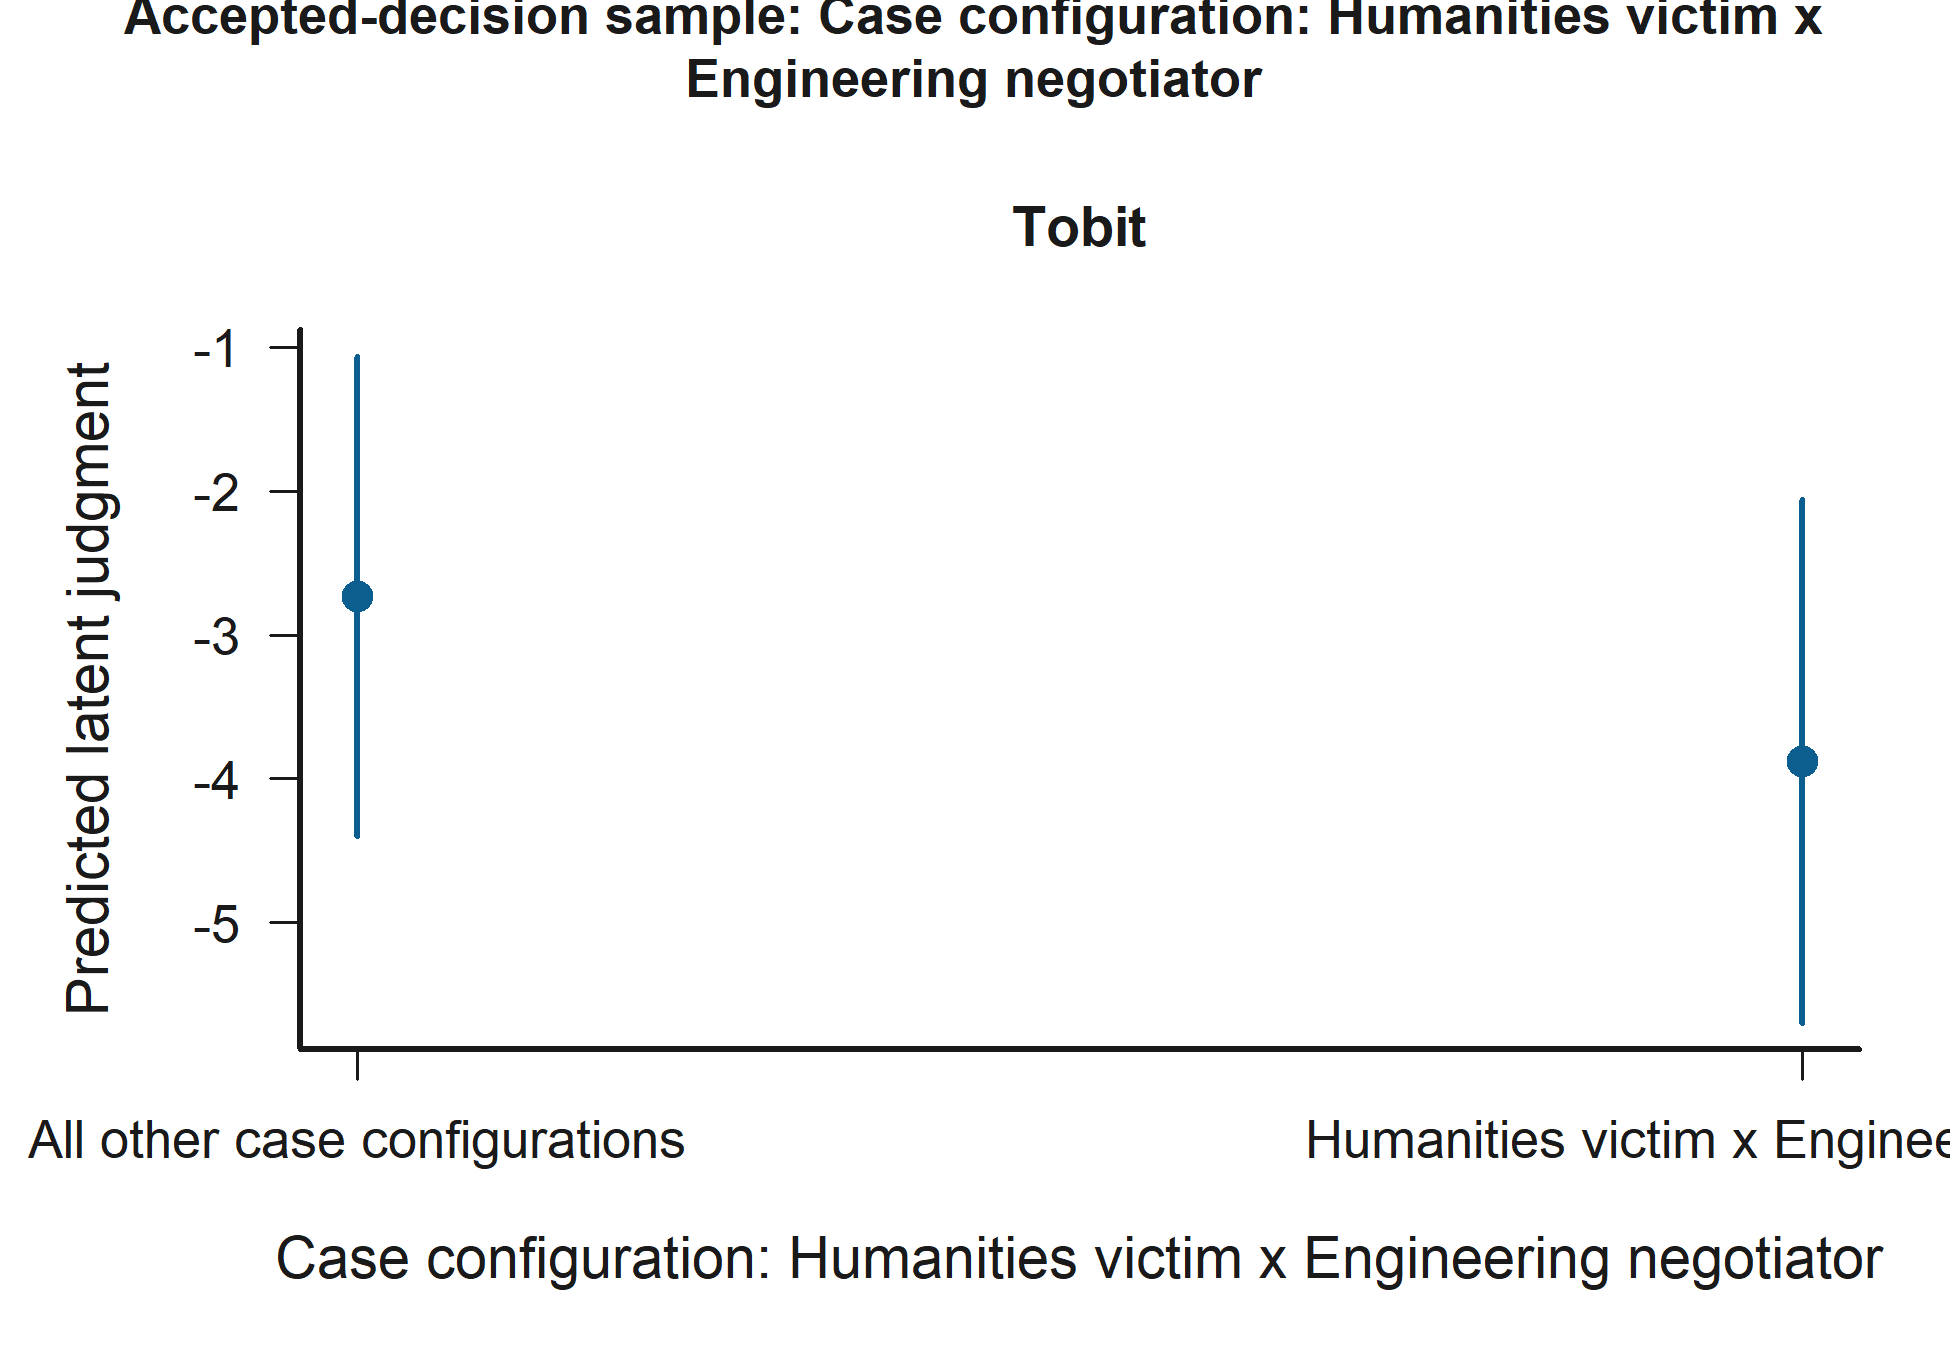
\includegraphics[width=0.92\textwidth]{../figures/figure_sig_all_accepted_decision_sample_case_hum_x_ing.png}
\caption{Grouped Prediction Plot for Case configuration: Humanities victim x Engineering negotiator in the Accepted-decision sample. Statistically significant support appears in H1: Empathy under explicit case configuration Model A (Tobit), H2b: Explicit case-configuration contrasts Model A (Tobit), H1: Empathy under explicit case configuration Model B (Tobit), and H2b: Explicit case-configuration contrasts Model B (Tobit). The panels show predicted latent judgments with 95\% confidence intervals.}
\label{fig:sig_all_accepted_decision_sample_case_hum_x_ing}
\end{figure}

Case configuration: Engineering victim x Humanities negotiator x Empathy composite (average) is statistically significant in H3: Empathy x case-configuration moderation Model A (Tobit). Figure \textbackslash\{\}ref\{fig:sig\_all\_accepted\_decision\_sample\_case\_ing\_x\_hum\_iri\_total\} shows that the predicted relationship falls most sharply for Empathy composite (average) when the condition is Engineering victim x Humanities negotiator.

\begin{figure}[H]
\centering
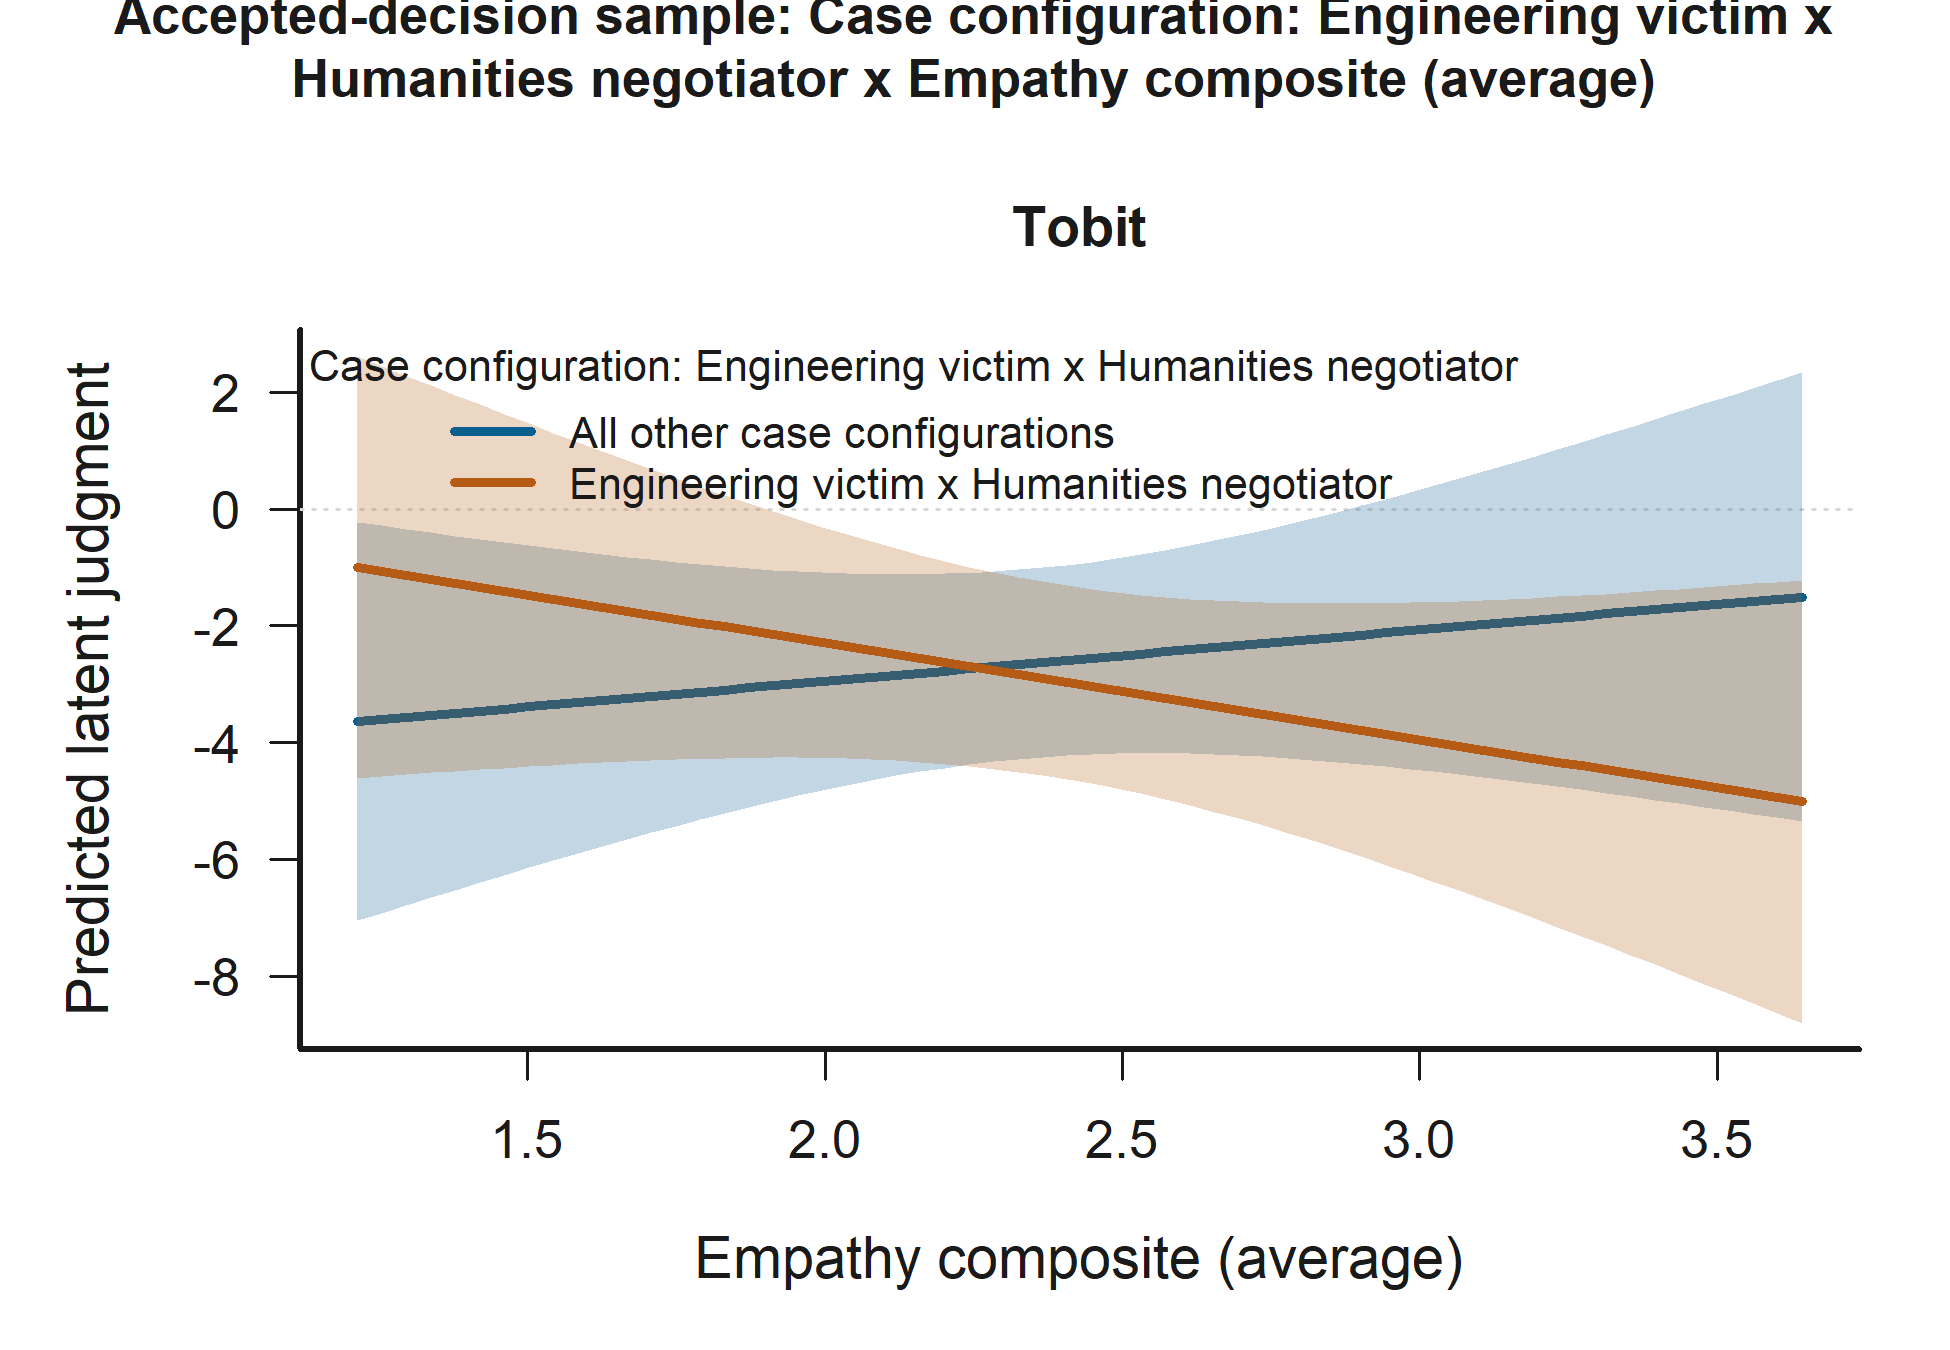
\includegraphics[width=0.92\textwidth]{../figures/figure_sig_all_accepted_decision_sample_case_ing_x_hum_iri_total.png}
\caption{Interaction Plot for Case configuration: Engineering victim x Humanities negotiator x Empathy composite (average) in the Accepted-decision sample. Statistically significant support appears in H3: Empathy x case-configuration moderation Model A (Tobit). The panels show predicted latent judgments with 95\% confidence intervals.}
\label{fig:sig_all_accepted_decision_sample_case_ing_x_hum_iri_total}
\end{figure}

Case configuration: Engineering victim x Humanities negotiator is statistically significant in H3: Empathy x case-configuration moderation Model A (Tobit). Figure \textbackslash\{\}ref\{fig:sig\_all\_accepted\_decision\_sample\_case\_ing\_x\_hum\} shows that predicted latent judgment is higher for Engineering victim x Humanities negotiator than for All other case configurations.

\begin{figure}[H]
\centering
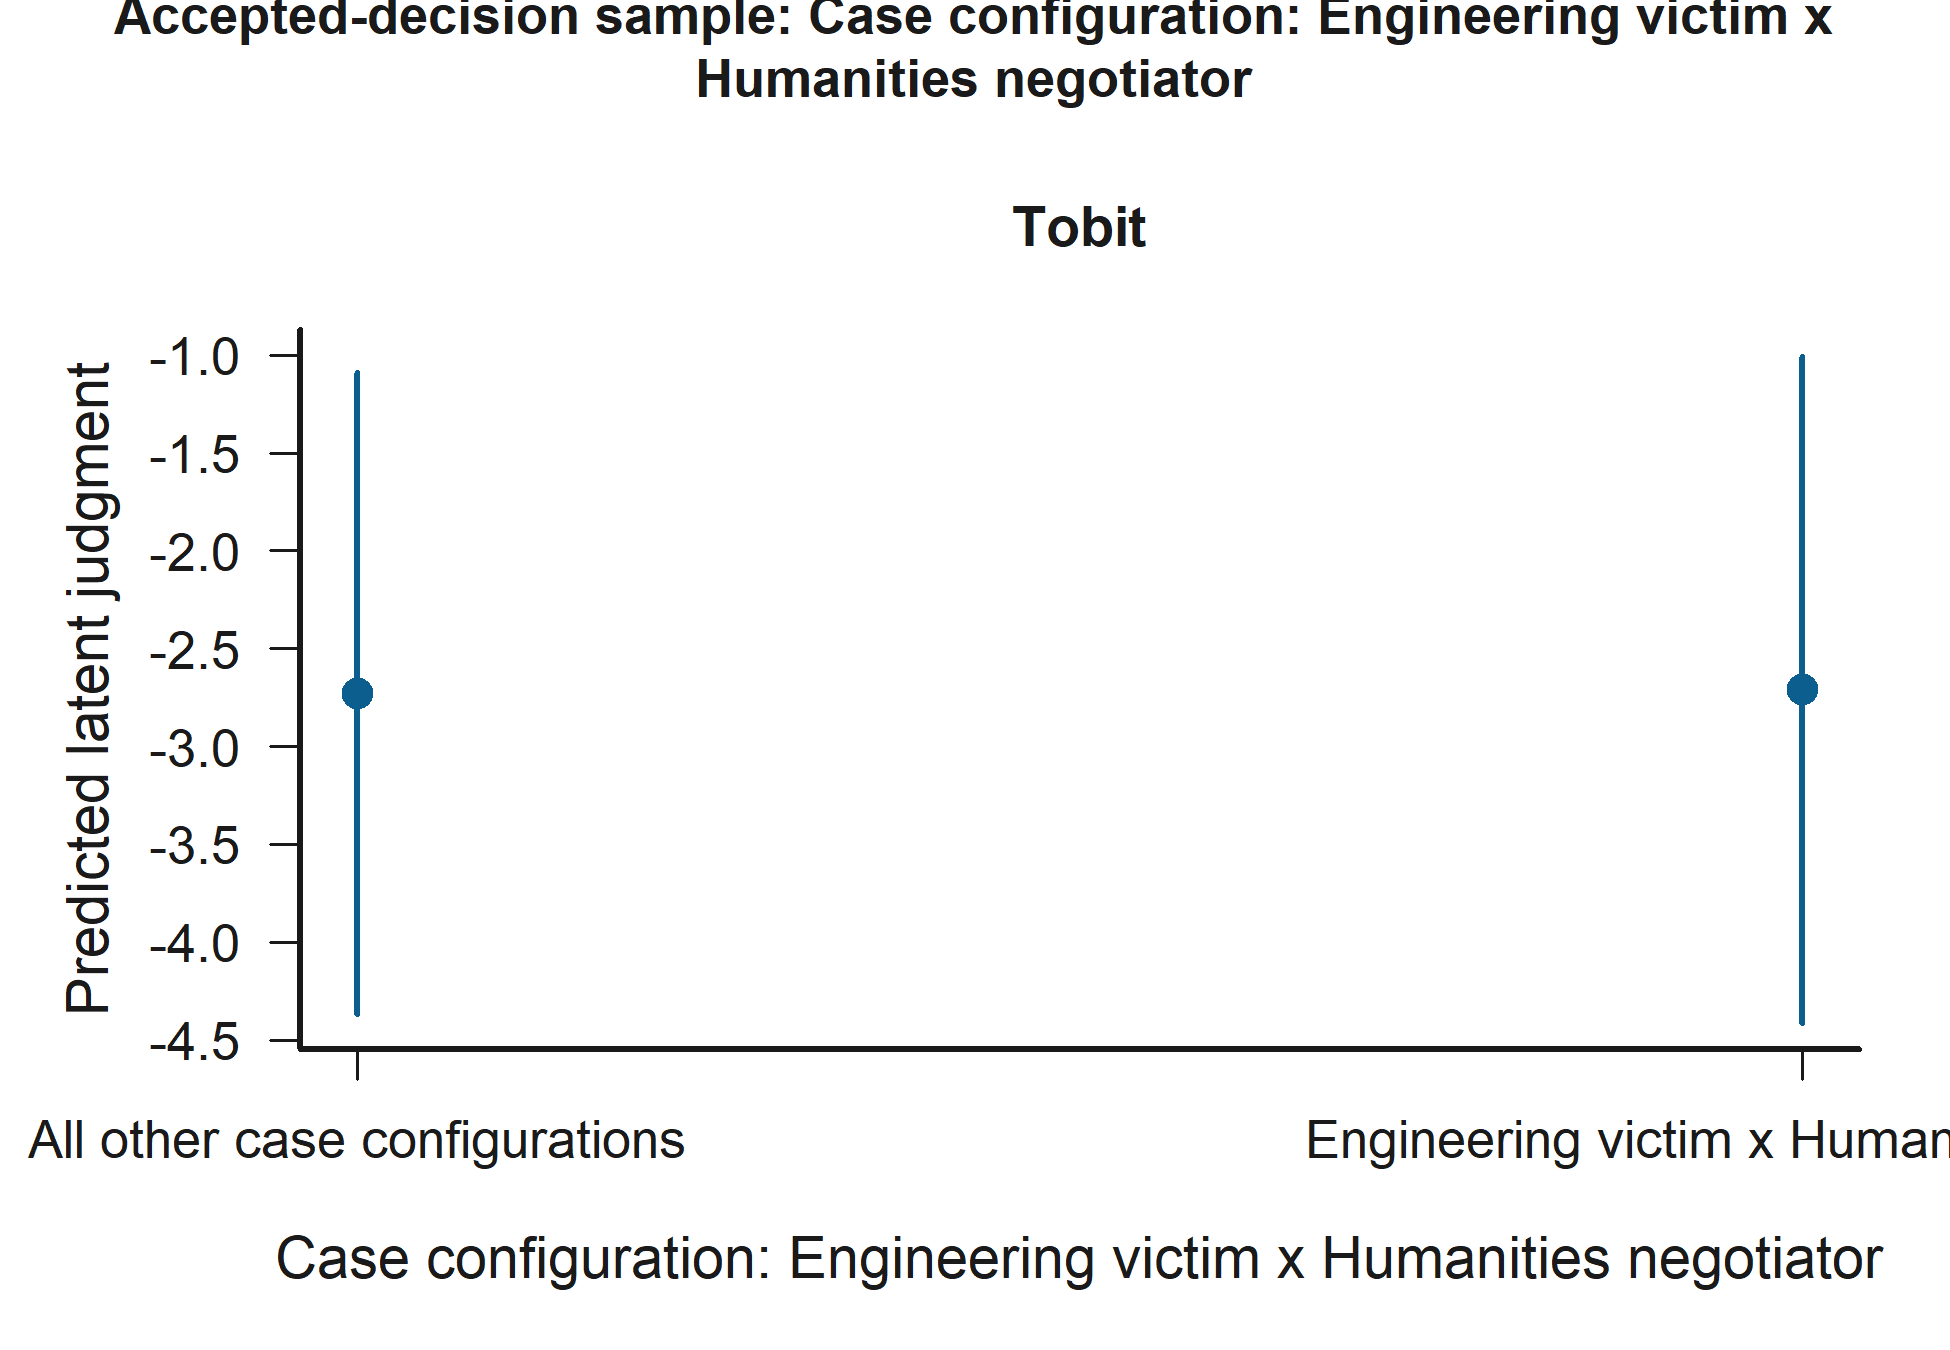
\includegraphics[width=0.92\textwidth]{../figures/figure_sig_all_accepted_decision_sample_case_ing_x_hum.png}
\caption{Grouped Prediction Plot for Case configuration: Engineering victim x Humanities negotiator in the Accepted-decision sample. Statistically significant support appears in H3: Empathy x case-configuration moderation Model A (Tobit). The panels show predicted latent judgments with 95\% confidence intervals.}
\label{fig:sig_all_accepted_decision_sample_case_ing_x_hum}
\end{figure}

\paragraph{Betrayal sample}

Observer role (ref = victim) is statistically significant in H2a: Relational betrayal contrasts Model A (Tobit) and H2a: Relational betrayal contrasts Model B (Tobit). Figure \textbackslash\{\}ref\{fig:sig\_all\_betrayal\_sample\_role\_observer\} shows that predicted latent judgment is higher for Observer role than for Victim role.

\begin{figure}[H]
\centering
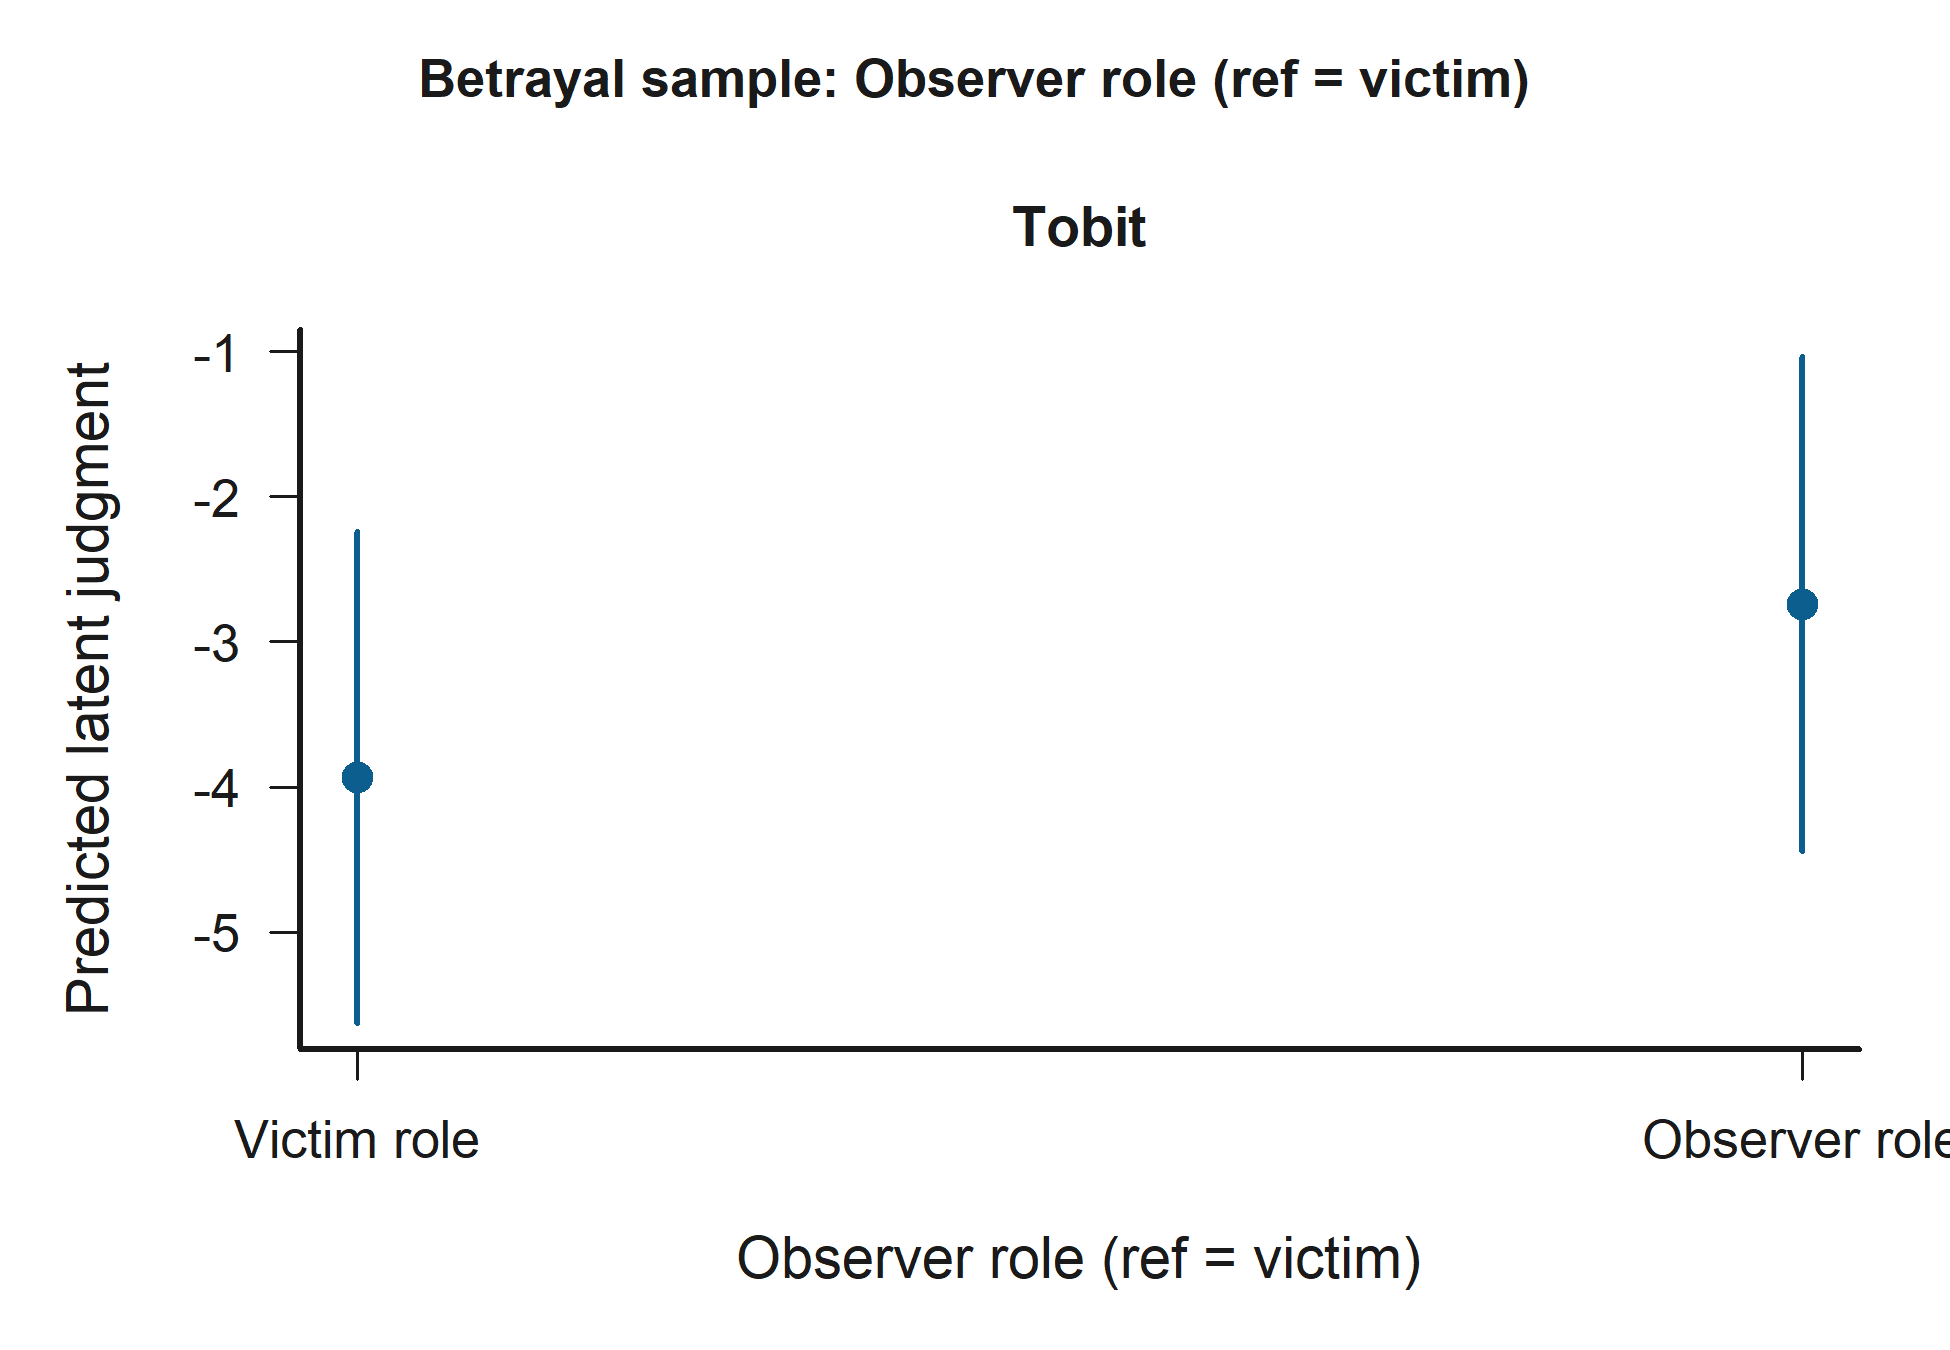
\includegraphics[width=0.92\textwidth]{../figures/figure_sig_all_betrayal_sample_role_observer.png}
\caption{Grouped Prediction Plot for Observer role (ref = victim) in the Betrayal sample. Statistically significant support appears in H2a: Relational betrayal contrasts Model A (Tobit) and H2a: Relational betrayal contrasts Model B (Tobit). The panels show predicted latent judgments with 95\% confidence intervals.}
\label{fig:sig_all_betrayal_sample_role_observer}
\end{figure}

Empathy: Empathic concern is statistically significant in H2a: Relational betrayal contrasts Model B (Tobit). Figure \textbackslash\{\}ref\{fig:sig\_all\_betrayal\_sample\_iri\_ec\} shows that across the observed range, higher Empathy: Empathic concern corresponds to lower predicted latent judgment.

\begin{figure}[H]
\centering
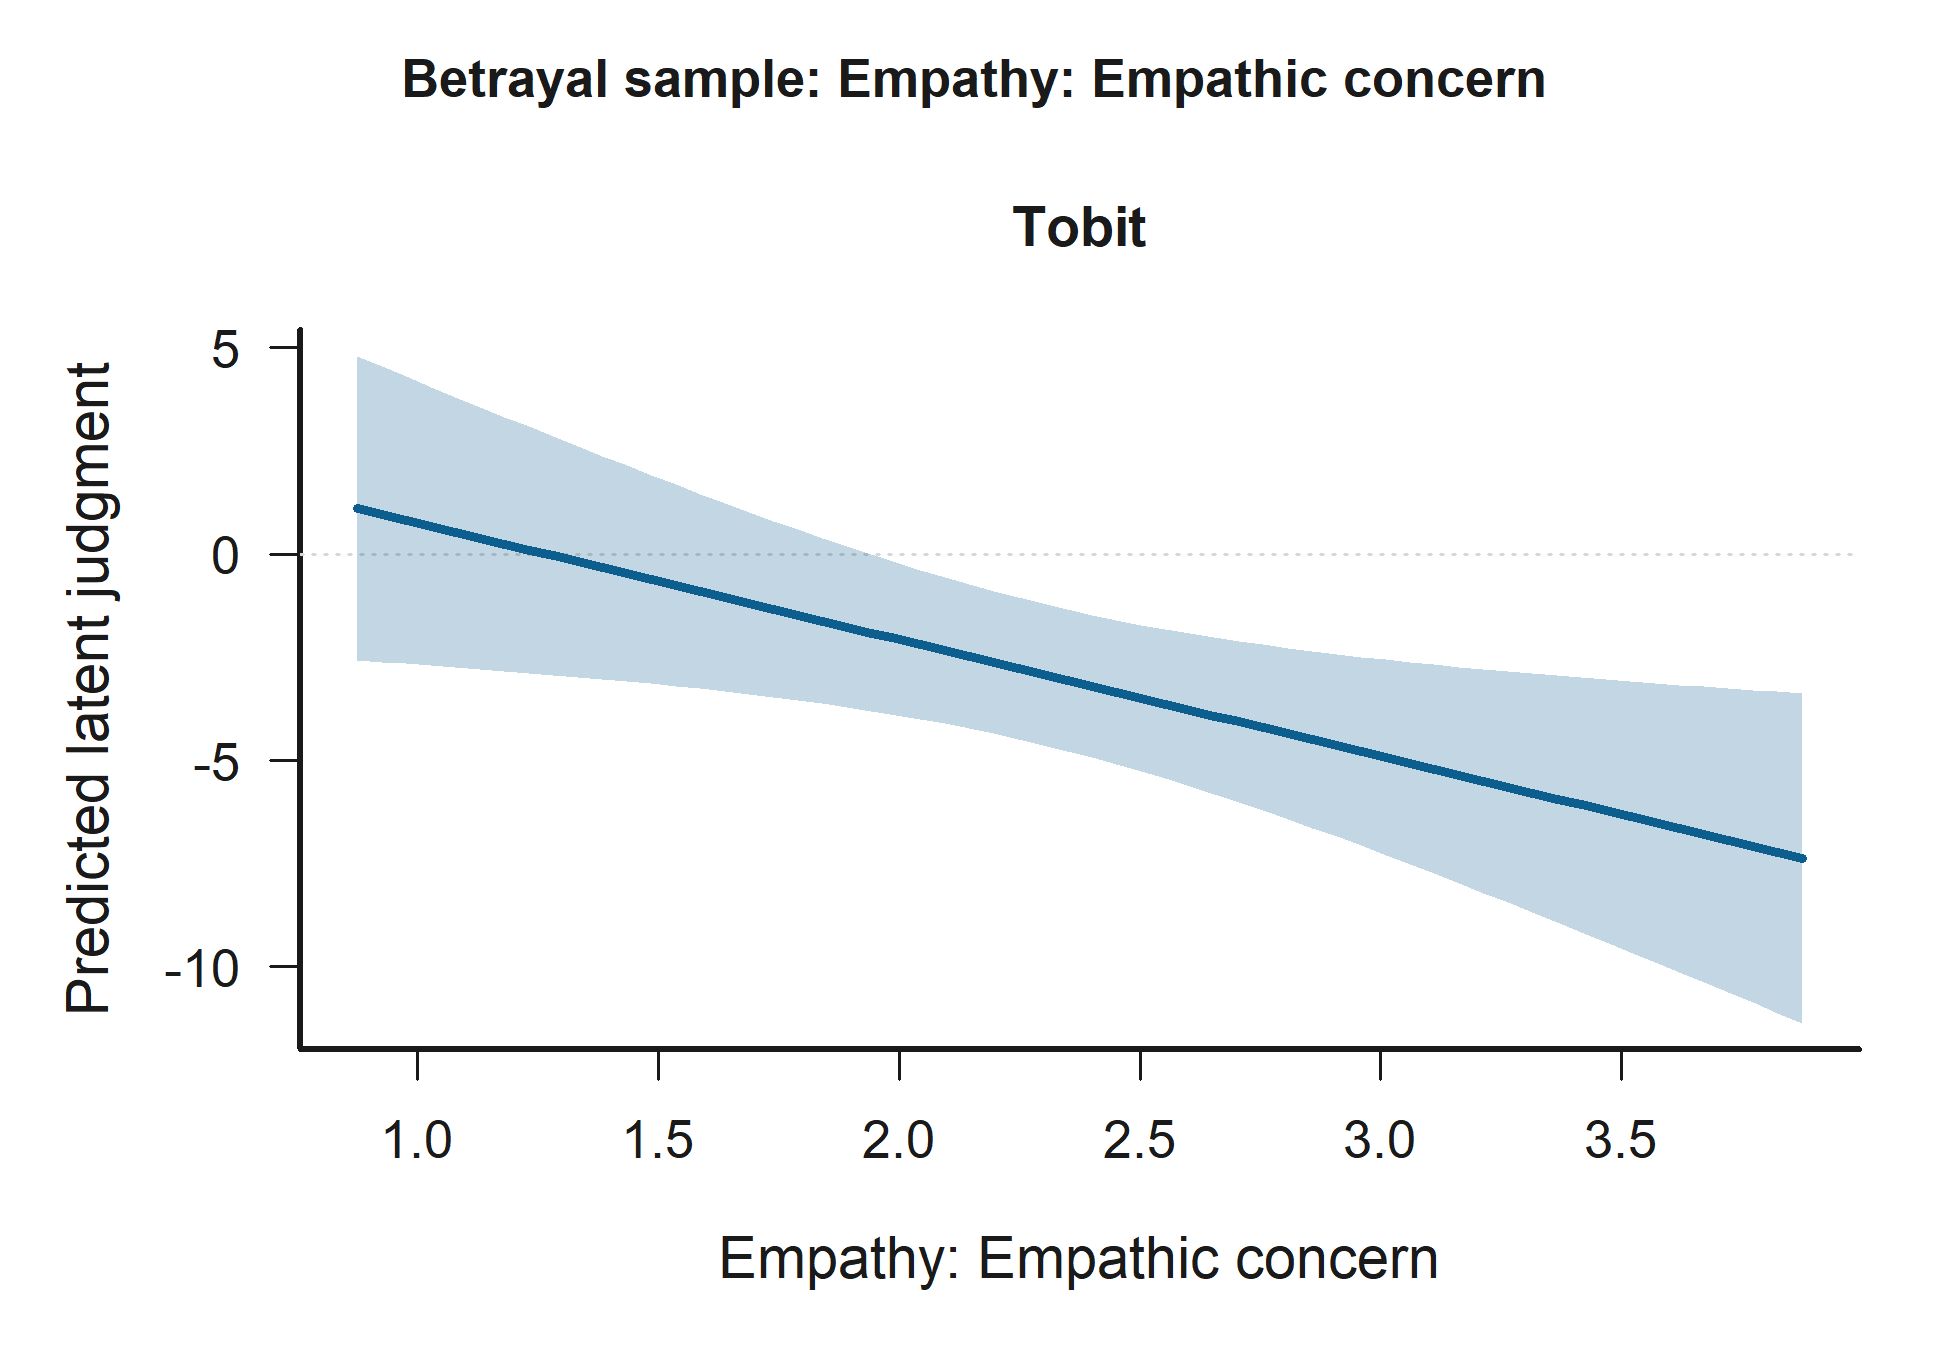
\includegraphics[width=0.92\textwidth]{../figures/figure_sig_all_betrayal_sample_iri_ec.png}
\caption{Effect Plot for Empathy: Empathic concern in the Betrayal sample. Statistically significant support appears in H2a: Relational betrayal contrasts Model B (Tobit). The panels show predicted latent judgments with 95\% confidence intervals.}
\label{fig:sig_all_betrayal_sample_iri_ec}
\end{figure}

Age is statistically significant in H2a: Relational betrayal contrasts Model A (Tobit) and H2a: Relational betrayal contrasts Model B (Tobit). Figure \textbackslash\{\}ref\{fig:sig\_all\_betrayal\_sample\_age\} shows that across the observed range, higher Age corresponds to higher predicted latent judgment.

\begin{figure}[H]
\centering
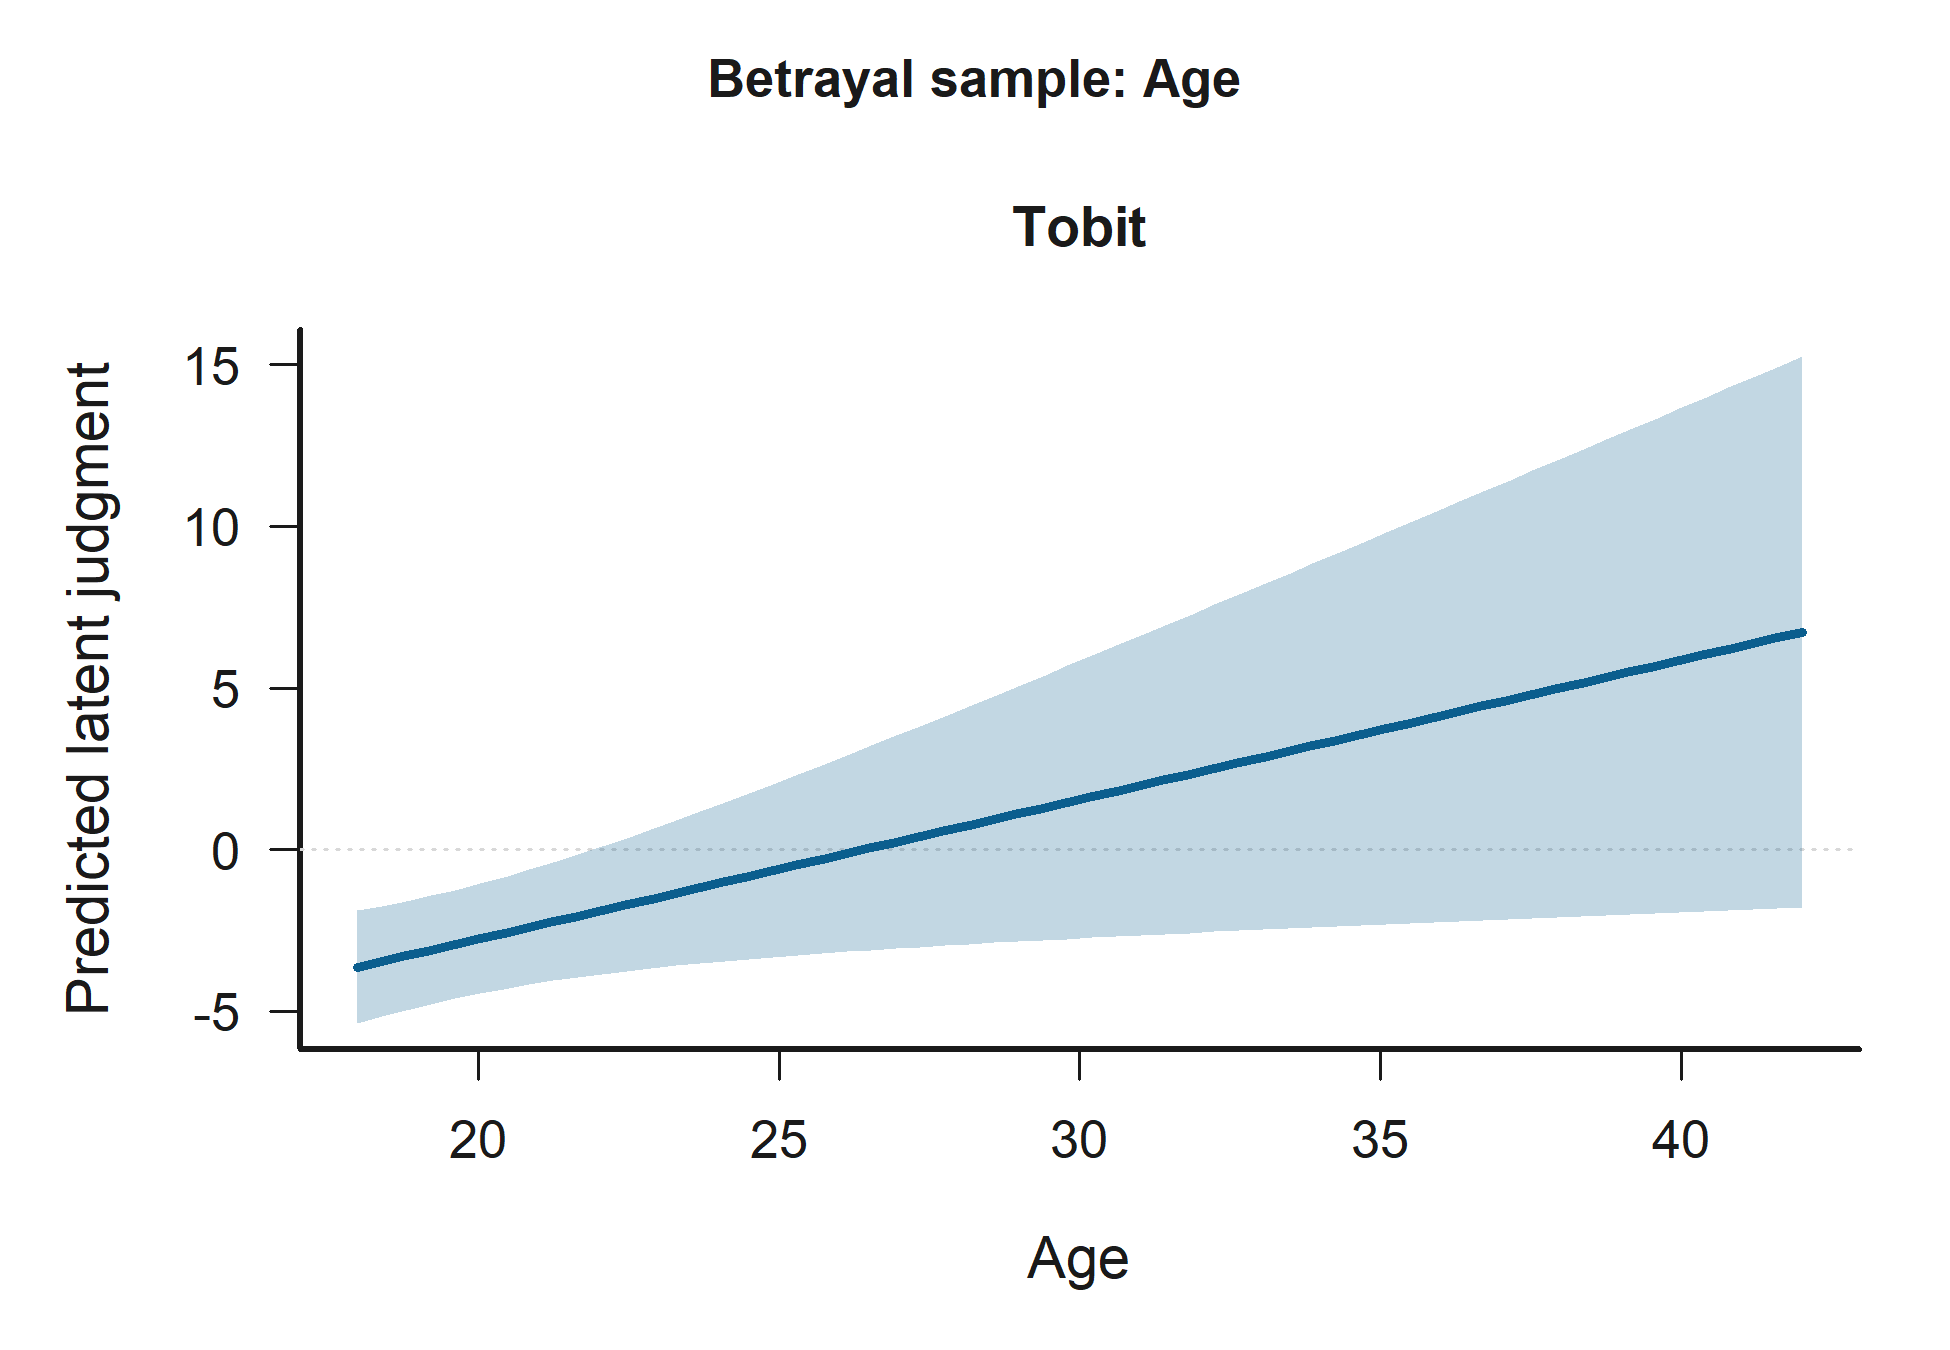
\includegraphics[width=0.92\textwidth]{../figures/figure_sig_all_betrayal_sample_age.png}
\caption{Effect Plot for Age in the Betrayal sample. Statistically significant support appears in H2a: Relational betrayal contrasts Model A (Tobit) and H2a: Relational betrayal contrasts Model B (Tobit). The panels show predicted latent judgments with 95\% confidence intervals.}
\label{fig:sig_all_betrayal_sample_age}
\end{figure}

Case configuration: Humanities victim x Engineering negotiator is statistically significant in H2a: Relational betrayal contrasts Model A (Tobit) and H2a: Relational betrayal contrasts Model B (Tobit). Figure \textbackslash\{\}ref\{fig:sig\_all\_betrayal\_sample\_case\_hum\_x\_ing\} shows that predicted latent judgment is lower for Humanities victim x Engineering negotiator than for All other case configurations.

\begin{figure}[H]
\centering
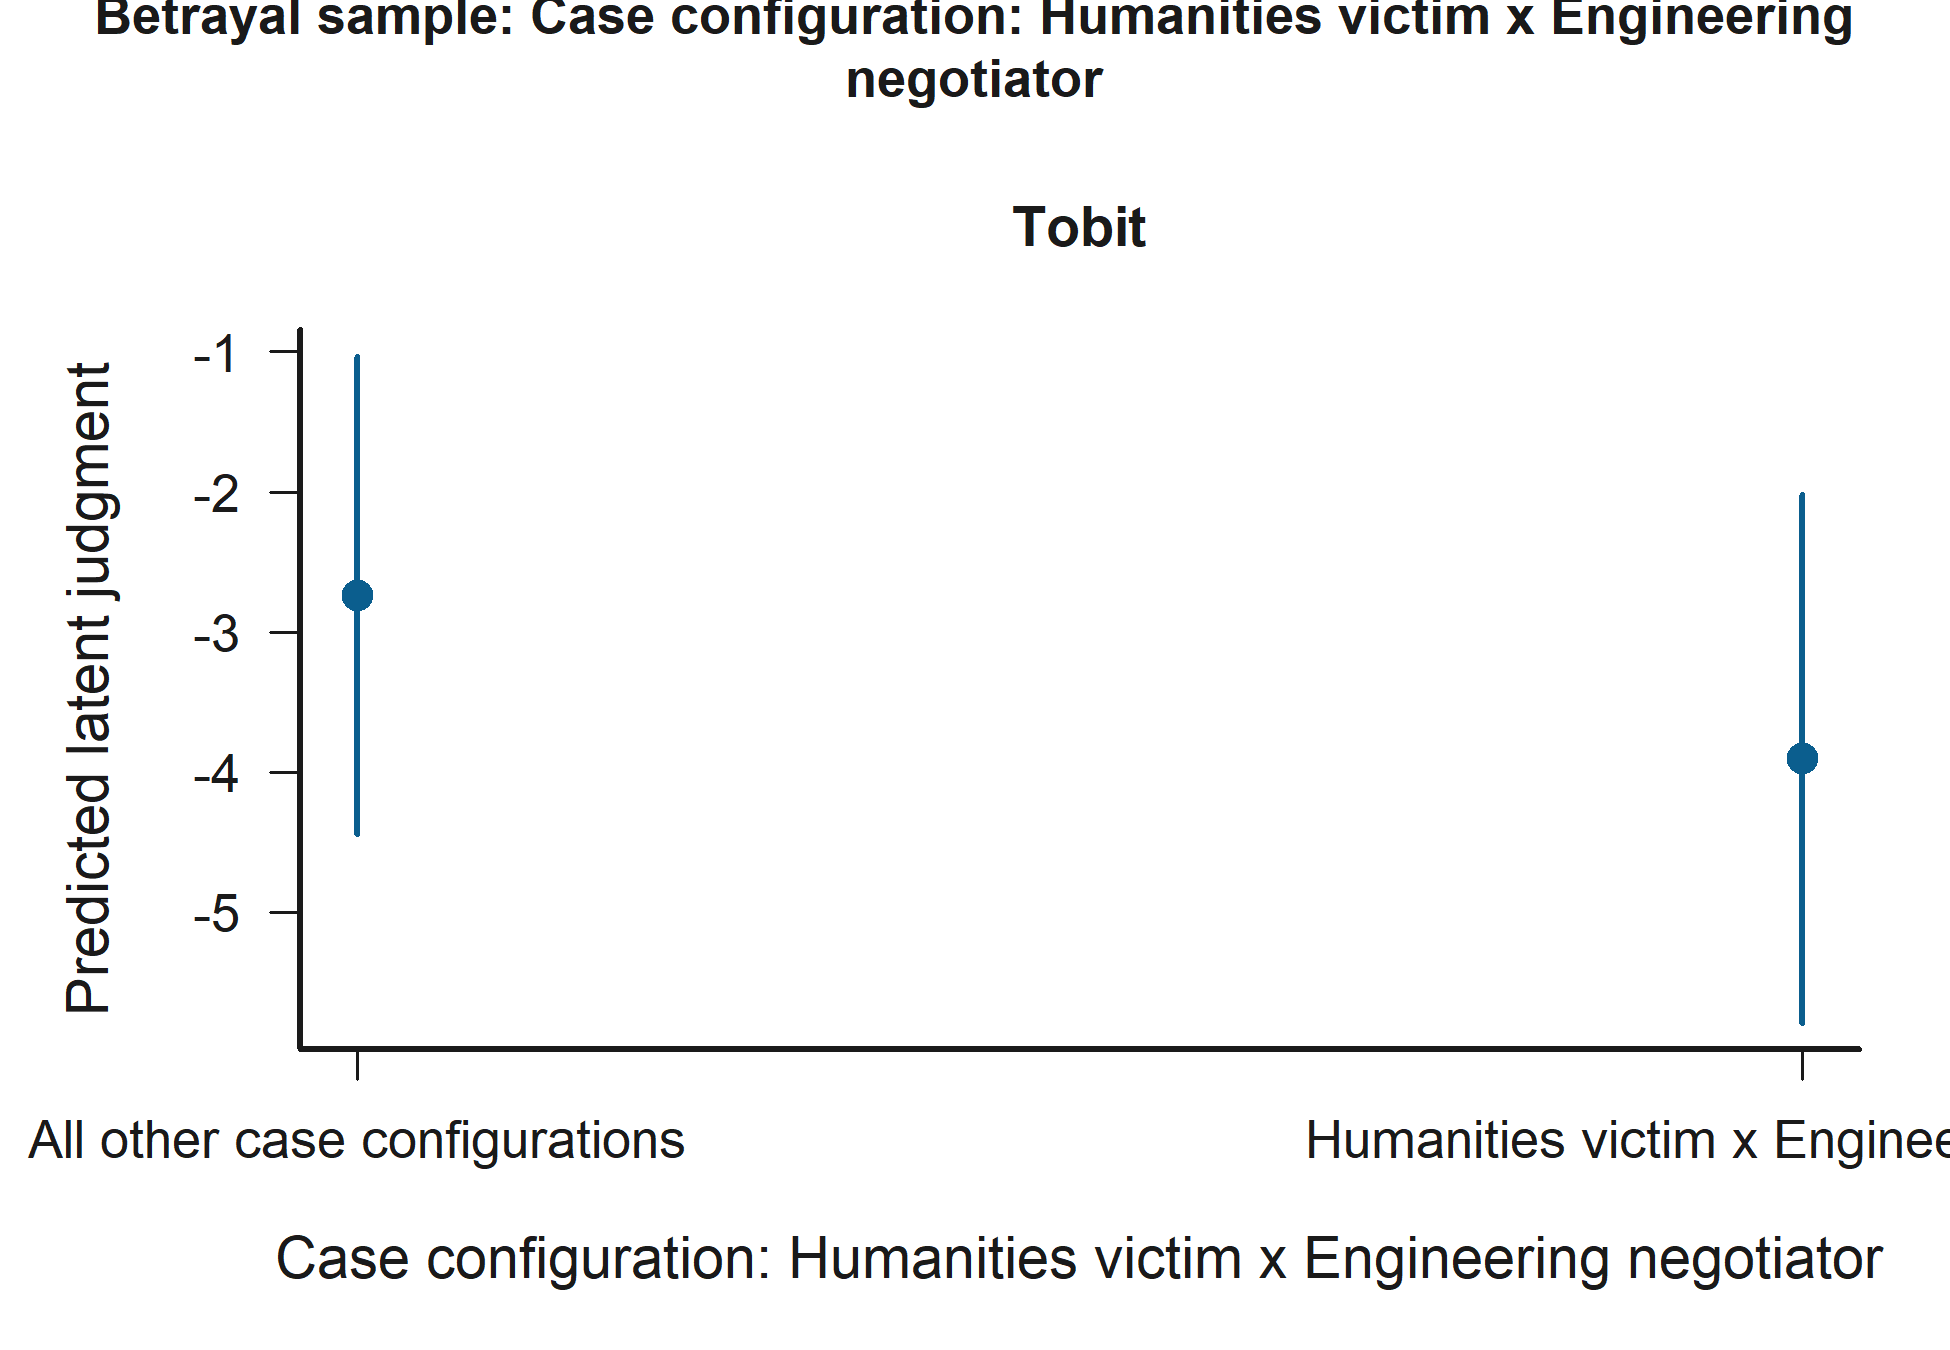
\includegraphics[width=0.92\textwidth]{../figures/figure_sig_all_betrayal_sample_case_hum_x_ing.png}
\caption{Grouped Prediction Plot for Case configuration: Humanities victim x Engineering negotiator in the Betrayal sample. Statistically significant support appears in H2a: Relational betrayal contrasts Model A (Tobit) and H2a: Relational betrayal contrasts Model B (Tobit). The panels show predicted latent judgments with 95\% confidence intervals.}
\label{fig:sig_all_betrayal_sample_case_hum_x_ing}
\end{figure}

Empathy: Perspective taking is statistically significant in H2a: Relational betrayal contrasts Model B (Tobit). Figure \textbackslash\{\}ref\{fig:sig\_all\_betrayal\_sample\_iri\_pt\} shows that across the observed range, higher Empathy: Perspective taking corresponds to higher predicted latent judgment.

\begin{figure}[H]
\centering
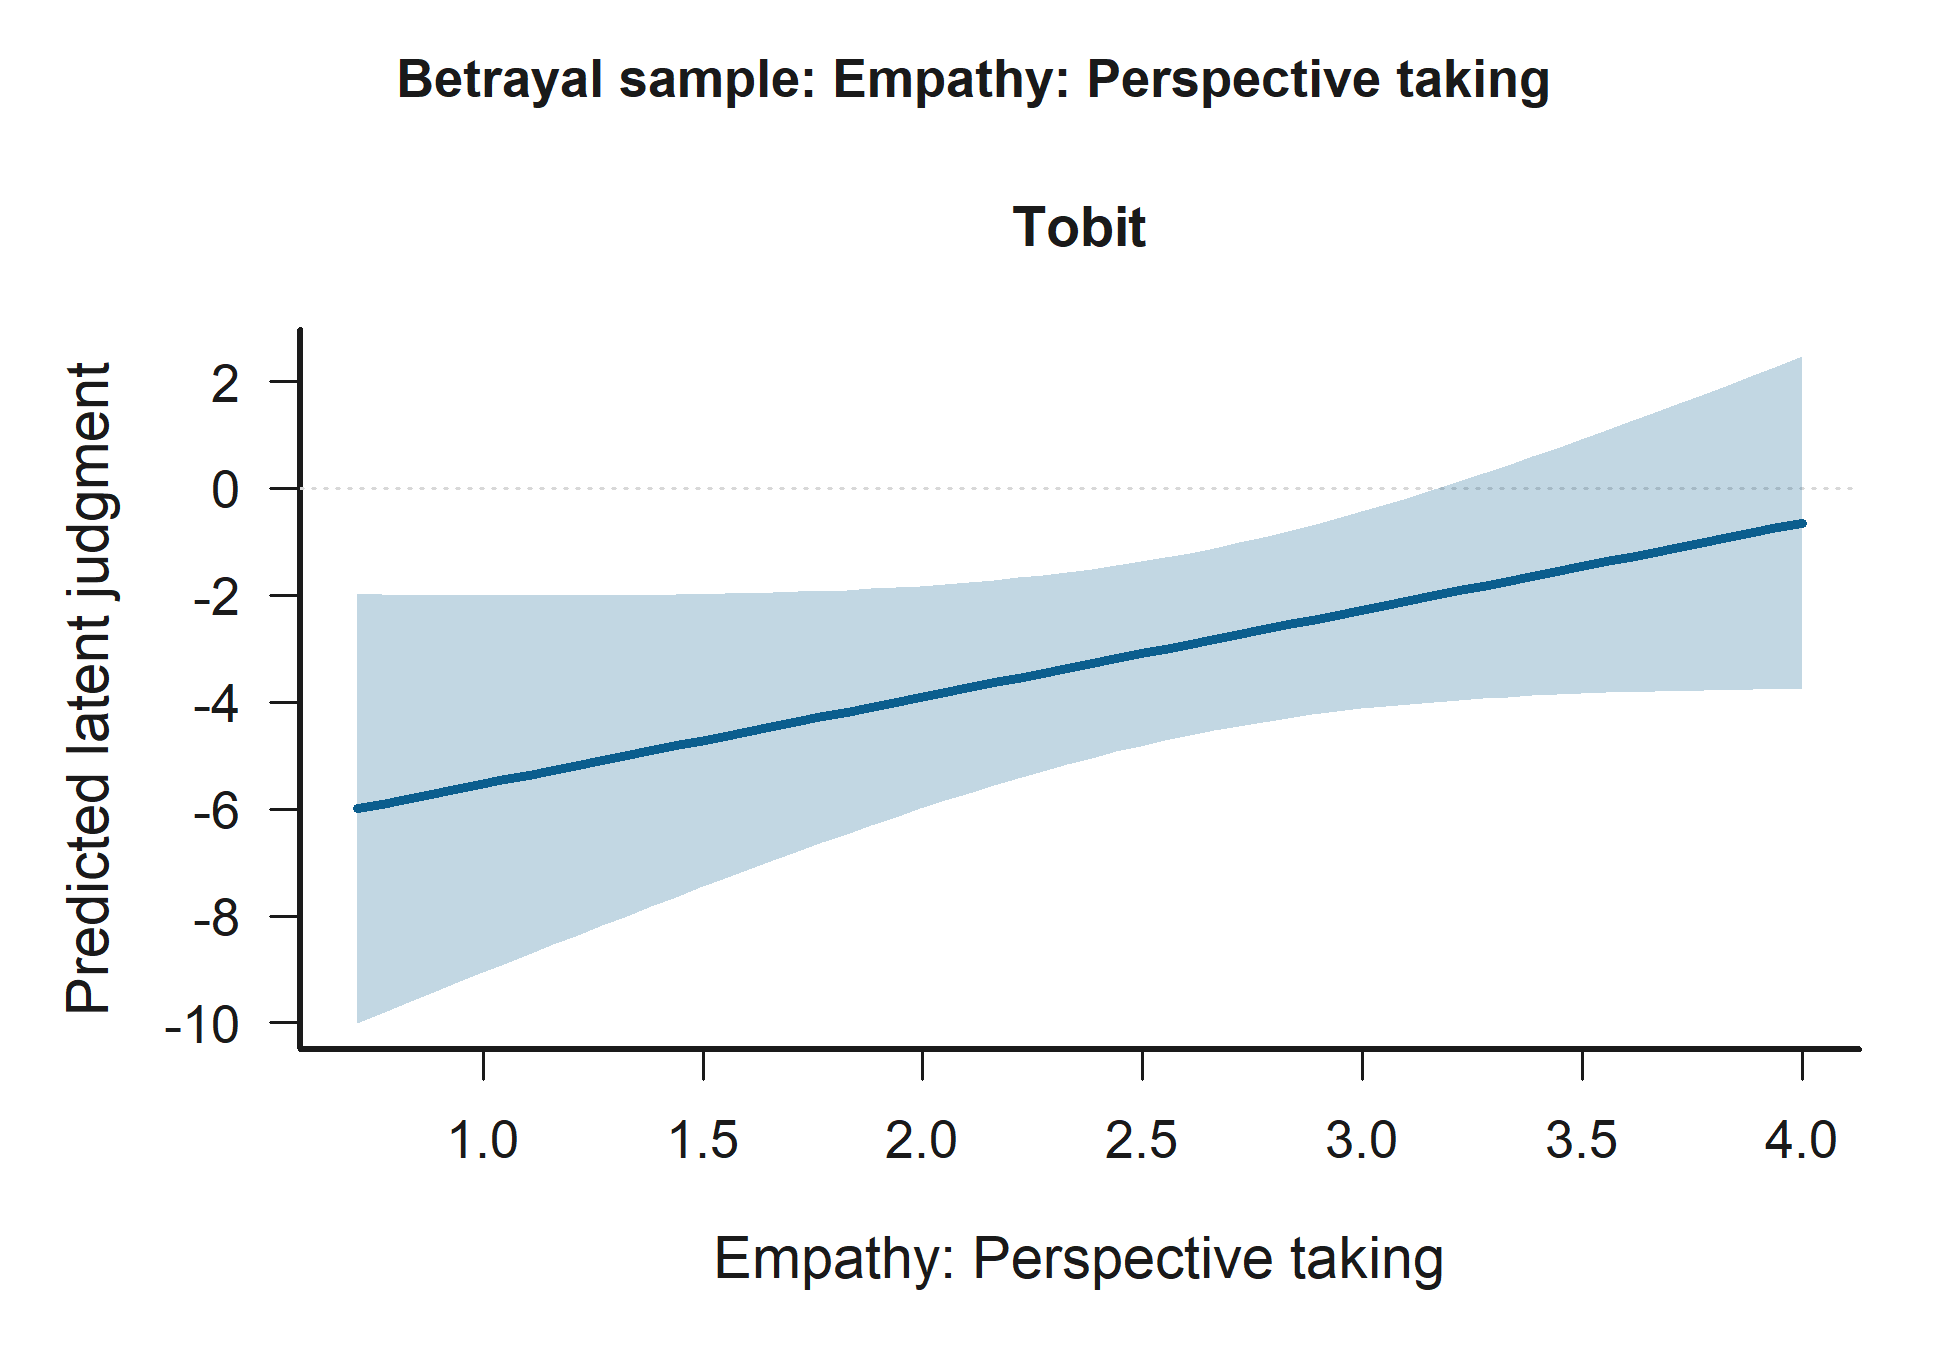
\includegraphics[width=0.92\textwidth]{../figures/figure_sig_all_betrayal_sample_iri_pt.png}
\caption{Effect Plot for Empathy: Perspective taking in the Betrayal sample. Statistically significant support appears in H2a: Relational betrayal contrasts Model B (Tobit). The panels show predicted latent judgments with 95\% confidence intervals.}
\label{fig:sig_all_betrayal_sample_iri_pt}
\end{figure}


\subsection{Integrated Hypothesis Conclusions}
The following summary restates each original hypothesis and indicates whether the available Tobit estimates and the cluster-aware non-parametric models support it in the current data. Non-parametric conclusions are drawn when the participant-level bootstrap inference is available and are otherwise labeled explicitly.
\begin{itemize}
\item H1. Original hypothesis: Higher empathy predicts lower moral-judgment scores for harmful decisions after conditioning on explicit victim x negotiator case configurations. Tobit conclusion: the evidence is mixed but offers partial support for the hypothesis. Model A does not support the hypothesis; Empathy composite (average) is negative but not statistically significant (p = 0.503). Model B supports the hypothesis through Empathy: Empathic concern with a negative association (p = 0.025). Additional statistically significant signals include Observer role (ref = victim) with a positive association (p = 0.004) and Age with a positive association (p = 0.035). Non-parametric conclusion: no converged second-phase non-parametric model is available, so the robustness check is inconclusive for this hypothesis.
\item H2a. Original hypothesis: Same-faculty and cross-faculty betrayal cases are evaluated through explicit victim x negotiator configurations rather than a single same\_group\_harm flag. Tobit conclusion: the available models do not support the hypothesis. Model A does not support the hypothesis; none of the betrayal-sample case-configuration contrasts are statistically significant, and the closest signal is Case configuration: Humanities victim x Engineering negotiator with a negative association (p = 0.061). Model B does not support the hypothesis; none of the betrayal-sample case-configuration contrasts are statistically significant, and the closest signal is Case configuration: Humanities victim x Engineering negotiator with a negative association (p = 0.097). Additional statistically significant signals include Observer role (ref = victim) with a positive association (p = 0.002) and Empathy: Empathic concern with a negative association (p = 0.016). Non-parametric conclusion: the full-sample non-parametric fit converged, but fewer than two participant-level bootstrap refits succeeded, so the robustness check is not interpreted inferentially for this hypothesis.
\item H2b. Original hypothesis: Relational judgments are interpreted through explicit victim x negotiator case configurations such as Hum\_x\_Ing, Hum\_x\_Control, Ing\_x\_Hum, Ing\_x\_Ing, and Ing\_x\_Control. Tobit conclusion: the available models do not support the hypothesis. Model A does not support the hypothesis; none of the accepted-sample case-configuration contrasts are statistically significant, and the closest signal is Case configuration: Humanities victim x Engineering negotiator with a negative association (p = 0.065). Model B does not support the hypothesis; none of the accepted-sample case-configuration contrasts are statistically significant, and the closest signal is Case configuration: Humanities victim x Engineering negotiator with a negative association (p = 0.095). Additional statistically significant signals include Observer role (ref = victim) with a positive association (p = 0.004) and Empathy: Empathic concern with a negative association (p = 0.025). Non-parametric conclusion: no converged second-phase non-parametric model is available, so the robustness check is inconclusive for this hypothesis.
\item H3. Original hypothesis: The empathy effect may vary across explicit victim x negotiator pairings, so moderation is modeled through empathy interactions with case-configuration contrasts. Tobit conclusion: the available models support the hypothesis. Model A supports the hypothesis through Case configuration: Humanities victim x Engineering negotiator x Empathy composite (average) with a negative association (p = 0.049). Model B supports the hypothesis through Case configuration: Engineering victim x Humanities negotiator x Empathy: Empathic concern with a negative association (p < 0.001) and Case configuration: Engineering victim x Humanities negotiator x Empathy: Personal distress with a positive association (p = 0.015). Additional statistically significant signals include Observer role (ref = victim) with a positive association (p = 0.004) and Age with a positive association (p = 0.032). Non-parametric conclusion: no converged second-phase non-parametric model is available, so the robustness check is inconclusive for this hypothesis.
\end{itemize}

\section{Hypothesis Validation and Results}
Detailed coefficient tables for each Tobit model, coupled with non-parametric robustness outputs, natural language interpretive narratives, and estimator-specific diagnostics, are provided below. In the default pipeline, converged non-parametric fits immediately attempt participant-level cluster-bootstrap inference; the report labels deferred and sparse-bootstrap cases explicitly when full inference is not available.

\subsection{H1: Empathy Effect}
This section evaluates the primary effect of empathy on moral judgments while holding explicit victim x negotiator case configurations constant.
\subsubsection{Model A: Composite Empathy}
\paragraph{Tobit Estimator}

\begin{table}[H]
\centering
\caption{H1 Model A: Composite Empathy Regression Coefficients (Tobit).}
\label{tab:h1_a}
\resizebox{\textwidth}{!}{%
\begin{tabular}{llll}
\toprule
label & estimate & std\_error & p\_value \\
\midrule
Intercept & -13.201 & 4.407 & 0.003 \\
Empathy composite (average) & -0.671 & 1.002 & 0.503 \\
Case configuration: Humanities victim x Engineering negotiator & -1.145 & 0.621 & 0.065 \\
Case configuration: Humanities victim x Control label hidden negotiator & -0.050 & 0.551 & 0.928 \\
Case configuration: Engineering victim x Humanities negotiator & 0.013 & 0.641 & 0.983 \\
Case configuration: Engineering victim x Engineering negotiator & -0.757 & 0.564 & 0.179 \\
Case configuration: Engineering victim x Control label hidden negotiator & 0.317 & 0.554 & 0.566 \\
Observer role (ref = victim) & 0.929 & 0.324 & 0.004 \\
Engineering participant (ref = humanities) & 1.415 & 0.889 & 0.111 \\
Man (ref = woman) & 0.356 & 0.892 & 0.690 \\
Age & 0.408 & 0.193 & 0.035 \\
Socioeconomic status & 0.267 & 0.392 & 0.495 \\
Negotiator 2 (ref = negotiator 1) & 0.621 & 0.261 & 0.017 \\
Scale variance (log) & 1.891 & 0.060 & 0.000 \\
\bottomrule
\end{tabular}
}
\end{table}

\textbf{Interpretation}

The Intercept represents the baseline latent moral judgment when all continuous predictors are zero and categorical predictors are at their reference levels. In this model, the baseline is estimated at -13.201 (p=0.003). The term iri\_total (representing the average composite of empathetic propensity across the participant) has an estimated $\beta$ coefficient of -0.671. The p-value of 0.503 indicates the effect is not statistically significant, meaning we do not have enough evidence to reject the null hypothesis for this vector. The term case\_hum\_x\_ing (representing whether the judged scenario matches the explicit victim x negotiator case configuration Humanities victim x Engineering negotiator) has an estimated $\beta$ coefficient of -1.145. The p-value of 0.065 indicates the effect is marginally significant, meaning we do not have enough evidence to reject the null hypothesis for this vector. The term case\_hum\_x\_control (representing whether the judged scenario matches the explicit victim x negotiator case configuration Humanities victim x Control label hidden negotiator) has an estimated $\beta$ coefficient of -0.050. The p-value of 0.928 indicates the effect is not statistically significant, meaning we do not have enough evidence to reject the null hypothesis for this vector. The term case\_ing\_x\_hum (representing whether the judged scenario matches the explicit victim x negotiator case configuration Engineering victim x Humanities negotiator) has an estimated $\beta$ coefficient of 0.013. The p-value of 0.983 indicates the effect is not statistically significant, meaning we do not have enough evidence to reject the null hypothesis for this vector. The term case\_ing\_x\_ing (representing whether the judged scenario matches the explicit victim x negotiator case configuration Engineering victim x Engineering negotiator) has an estimated $\beta$ coefficient of -0.757. The p-value of 0.179 indicates the effect is not statistically significant, meaning we do not have enough evidence to reject the null hypothesis for this vector. The term case\_ing\_x\_control (representing whether the judged scenario matches the explicit victim x negotiator case configuration Engineering victim x Control label hidden negotiator) has an estimated $\beta$ coefficient of 0.317. The p-value of 0.566 indicates the effect is not statistically significant, meaning we do not have enough evidence to reject the null hypothesis for this vector. The term role\_observer (representing the procedural role where the participant acted exclusively as an observer rather than a victim) has an estimated $\beta$ coefficient of 0.929. The p-value of 0.004 indicates statistically significant, meaning the predictor has a positive effect on the latent moral judgment. The term participant\_engineering (representing whether the participant belonged to the Engineering faculty as opposed to Humanities) has an estimated $\beta$ coefficient of 1.415. The p-value of 0.111 indicates the effect is not statistically significant, meaning we do not have enough evidence to reject the null hypothesis for this vector. The term sex\_man (representing whether the participant identified as a man instead of a woman) has an estimated $\beta$ coefficient of 0.356. The p-value of 0.690 indicates the effect is not statistically significant, meaning we do not have enough evidence to reject the null hypothesis for this vector. The term age (representing the participant's biological age in years) has an estimated $\beta$ coefficient of 0.408. The p-value of 0.035 indicates statistically significant, meaning the predictor has a positive effect on the latent moral judgment. The term economic\_status (representing the socioeconomic contextual stratum of the participant's background) has an estimated $\beta$ coefficient of 0.267. The p-value of 0.495 indicates the effect is not statistically significant, meaning we do not have enough evidence to reject the null hypothesis for this vector. The Log(scale) is a standard Tobit variance parameter representing the natural logarithm of the standard deviation of the unobserved residuals. The estimated scale parameter log is 1.891, capturing the underlying dispersion of latent judgments.

\textbf{Diagnostics}

The Shapiro-Wilk test on the deviance residuals indicates a violation of the normality assumption (W = 0.954, p = 3.779e-24). The primary Tobit model still uses participant-clustered standard errors by id, and the report pairs it with a cluster-bootstrap non-parametric censored robustness model.


\paragraph{Non-parametric Robustness Estimator}

\begin{table}[H]
\centering
\caption{H1 Model A: Composite Empathy Regression Coefficients (cluster-aware non-parametric robustness).}
\label{tab:h1_a_clad}
\resizebox{\textwidth}{!}{%
\begin{tabular}{lll}
\toprule
label & estimate & inference \\
\midrule
Intercept & -15.801 & Cluster bootstrap skipped because the full-sample non-parametric fit did not converge \\
Empathy composite (average) & -0.447 & Cluster bootstrap skipped because the full-sample non-parametric fit did not converge \\
Case configuration: Humanities victim x Engineering negotiator & -0.892 & Cluster bootstrap skipped because the full-sample non-parametric fit did not converge \\
Case configuration: Humanities victim x Control label hidden negotiator & -0.164 & Cluster bootstrap skipped because the full-sample non-parametric fit did not converge \\
Case configuration: Engineering victim x Humanities negotiator & -0.147 & Cluster bootstrap skipped because the full-sample non-parametric fit did not converge \\
Case configuration: Engineering victim x Engineering negotiator & -0.418 & Cluster bootstrap skipped because the full-sample non-parametric fit did not converge \\
Case configuration: Engineering victim x Control label hidden negotiator & 0.090 & Cluster bootstrap skipped because the full-sample non-parametric fit did not converge \\
Observer role (ref = victim) & 0.999 & Cluster bootstrap skipped because the full-sample non-parametric fit did not converge \\
Engineering participant (ref = humanities) & -0.129 & Cluster bootstrap skipped because the full-sample non-parametric fit did not converge \\
Man (ref = woman) & 0.175 & Cluster bootstrap skipped because the full-sample non-parametric fit did not converge \\
Age & 0.615 & Cluster bootstrap skipped because the full-sample non-parametric fit did not converge \\
Socioeconomic status & 0.012 & Cluster bootstrap skipped because the full-sample non-parametric fit did not converge \\
Negotiator 2 (ref = negotiator 1) & 0.271 & Cluster bootstrap skipped because the full-sample non-parametric fit did not converge \\
\bottomrule
\end{tabular}
}
\end{table}

\textbf{Interpretation}

The Intercept represents the baseline conditional median latent moral judgment when all continuous predictors are zero and categorical predictors are at their reference levels. In this model, that baseline median is estimated at -15.801 (p=NA). The term iri\_total (representing the average composite of empathetic propensity across the participant) has an estimated $\beta$ coefficient of -0.447. The p-value of NA the p-value cannot be determined. The term case\_hum\_x\_ing (representing whether the judged scenario matches the explicit victim x negotiator case configuration Humanities victim x Engineering negotiator) has an estimated $\beta$ coefficient of -0.892. The p-value of NA the p-value cannot be determined. The term case\_hum\_x\_control (representing whether the judged scenario matches the explicit victim x negotiator case configuration Humanities victim x Control label hidden negotiator) has an estimated $\beta$ coefficient of -0.164. The p-value of NA the p-value cannot be determined. The term case\_ing\_x\_hum (representing whether the judged scenario matches the explicit victim x negotiator case configuration Engineering victim x Humanities negotiator) has an estimated $\beta$ coefficient of -0.147. The p-value of NA the p-value cannot be determined. The term case\_ing\_x\_ing (representing whether the judged scenario matches the explicit victim x negotiator case configuration Engineering victim x Engineering negotiator) has an estimated $\beta$ coefficient of -0.418. The p-value of NA the p-value cannot be determined. The term case\_ing\_x\_control (representing whether the judged scenario matches the explicit victim x negotiator case configuration Engineering victim x Control label hidden negotiator) has an estimated $\beta$ coefficient of 0.090. The p-value of NA the p-value cannot be determined. The term role\_observer (representing the procedural role where the participant acted exclusively as an observer rather than a victim) has an estimated $\beta$ coefficient of 0.999. The p-value of NA the p-value cannot be determined. The term participant\_engineering (representing whether the participant belonged to the Engineering faculty as opposed to Humanities) has an estimated $\beta$ coefficient of -0.129. The p-value of NA the p-value cannot be determined. The term sex\_man (representing whether the participant identified as a man instead of a woman) has an estimated $\beta$ coefficient of 0.175. The p-value of NA the p-value cannot be determined. The term age (representing the participant's biological age in years) has an estimated $\beta$ coefficient of 0.615. The p-value of NA the p-value cannot be determined. The term economic\_status (representing the socioeconomic contextual stratum of the participant's background) has an estimated $\beta$ coefficient of 0.012. The p-value of NA the p-value cannot be determined.

\textbf{Diagnostics}

The non-parametric robustness model did not achieve convergence in the full sample after 2000 iterations, so participant-level cluster bootstrap inference was not attempted for this specification. The reported point estimates remain on the original judgement scale because the internal response shift of 10.0 units was back-transformed.

\subsubsection{Model B: Separated Empathy Constructs}
\paragraph{Tobit Estimator}

\begin{table}[H]
\centering
\caption{H1 Model B: Separated Constructs Regression Coefficients (Tobit).}
\label{tab:h1_b}
\resizebox{\textwidth}{!}{%
\begin{tabular}{llll}
\toprule
label & estimate & std\_error & p\_value \\
\midrule
Intercept & -12.864 & 4.619 & 0.005 \\
Empathy: Fantasy scale & -0.930 & 0.804 & 0.247 \\
Empathy: Empathic concern & -2.523 & 1.123 & 0.025 \\
Empathy: Perspective taking & 1.738 & 0.857 & 0.042 \\
Empathy: Personal distress & 1.291 & 0.965 & 0.181 \\
Case configuration: Humanities victim x Engineering negotiator & -1.030 & 0.617 & 0.095 \\
Case configuration: Humanities victim x Control label hidden negotiator & -0.094 & 0.552 & 0.865 \\
Case configuration: Engineering victim x Humanities negotiator & 0.071 & 0.639 & 0.912 \\
Case configuration: Engineering victim x Engineering negotiator & -0.684 & 0.561 & 0.223 \\
Case configuration: Engineering victim x Control label hidden negotiator & 0.312 & 0.545 & 0.567 \\
Observer role (ref = victim) & 0.912 & 0.327 & 0.005 \\
Engineering participant (ref = humanities) & 1.377 & 0.914 & 0.132 \\
Man (ref = woman) & 0.241 & 0.946 & 0.799 \\
Age & 0.368 & 0.195 & 0.059 \\
Socioeconomic status & 0.126 & 0.393 & 0.748 \\
Negotiator 2 (ref = negotiator 1) & 0.532 & 0.255 & 0.037 \\
Scale variance (log) & 1.876 & 0.057 & 0.000 \\
\bottomrule
\end{tabular}
}
\end{table}

\textbf{Interpretation}

The Intercept represents the baseline latent moral judgment when all continuous predictors are zero and categorical predictors are at their reference levels. In this model, the baseline is estimated at -12.864 (p=0.005). The term iri\_fs (representing the participant's inclination to transpose themselves imaginatively into the feelings of fictitious characters (Fantasy scale)) has an estimated $\beta$ coefficient of -0.930. The p-value of 0.247 indicates the effect is not statistically significant, meaning we do not have enough evidence to reject the null hypothesis for this vector. The term iri\_ec (representing the participant's tendency to experience feelings of sympathy and compassion for unfortunate others (Empathic Concern)) has an estimated $\beta$ coefficient of -2.523. The p-value of 0.025 indicates statistically significant, meaning the predictor has a negative effect on the latent moral judgment. The term iri\_pt (representing the participant's tendency to spontaneously adopt the psychological point of view of others (Perspective Taking)) has an estimated $\beta$ coefficient of 1.738. The p-value of 0.042 indicates statistically significant, meaning the predictor has a positive effect on the latent moral judgment. The term iri\_pd (representing the participant's tendency to experience distress and discomfort in tense interpersonal settings (Personal Distress)) has an estimated $\beta$ coefficient of 1.291. The p-value of 0.181 indicates the effect is not statistically significant, meaning we do not have enough evidence to reject the null hypothesis for this vector. The term case\_hum\_x\_ing (representing whether the judged scenario matches the explicit victim x negotiator case configuration Humanities victim x Engineering negotiator) has an estimated $\beta$ coefficient of -1.030. The p-value of 0.095 indicates the effect is marginally significant, meaning we do not have enough evidence to reject the null hypothesis for this vector. The term case\_hum\_x\_control (representing whether the judged scenario matches the explicit victim x negotiator case configuration Humanities victim x Control label hidden negotiator) has an estimated $\beta$ coefficient of -0.094. The p-value of 0.865 indicates the effect is not statistically significant, meaning we do not have enough evidence to reject the null hypothesis for this vector. The term case\_ing\_x\_hum (representing whether the judged scenario matches the explicit victim x negotiator case configuration Engineering victim x Humanities negotiator) has an estimated $\beta$ coefficient of 0.071. The p-value of 0.912 indicates the effect is not statistically significant, meaning we do not have enough evidence to reject the null hypothesis for this vector. The term case\_ing\_x\_ing (representing whether the judged scenario matches the explicit victim x negotiator case configuration Engineering victim x Engineering negotiator) has an estimated $\beta$ coefficient of -0.684. The p-value of 0.223 indicates the effect is not statistically significant, meaning we do not have enough evidence to reject the null hypothesis for this vector. The term case\_ing\_x\_control (representing whether the judged scenario matches the explicit victim x negotiator case configuration Engineering victim x Control label hidden negotiator) has an estimated $\beta$ coefficient of 0.312. The p-value of 0.567 indicates the effect is not statistically significant, meaning we do not have enough evidence to reject the null hypothesis for this vector. The term role\_observer (representing the procedural role where the participant acted exclusively as an observer rather than a victim) has an estimated $\beta$ coefficient of 0.912. The p-value of 0.005 indicates statistically significant, meaning the predictor has a positive effect on the latent moral judgment. The term participant\_engineering (representing whether the participant belonged to the Engineering faculty as opposed to Humanities) has an estimated $\beta$ coefficient of 1.377. The p-value of 0.132 indicates the effect is not statistically significant, meaning we do not have enough evidence to reject the null hypothesis for this vector. The term sex\_man (representing whether the participant identified as a man instead of a woman) has an estimated $\beta$ coefficient of 0.241. The p-value of 0.799 indicates the effect is not statistically significant, meaning we do not have enough evidence to reject the null hypothesis for this vector. The term age (representing the participant's biological age in years) has an estimated $\beta$ coefficient of 0.368. The p-value of 0.059 indicates the effect is marginally significant, meaning we do not have enough evidence to reject the null hypothesis for this vector. The term economic\_status (representing the socioeconomic contextual stratum of the participant's background) has an estimated $\beta$ coefficient of 0.126. The p-value of 0.748 indicates the effect is not statistically significant, meaning we do not have enough evidence to reject the null hypothesis for this vector. The Log(scale) is a standard Tobit variance parameter representing the natural logarithm of the standard deviation of the unobserved residuals. The estimated scale parameter log is 1.876, capturing the underlying dispersion of latent judgments.

\textbf{Diagnostics}

The Shapiro-Wilk test on the deviance residuals indicates a violation of the normality assumption (W = 0.963, p = 9.425e-22). The primary Tobit model still uses participant-clustered standard errors by id, and the report pairs it with a cluster-bootstrap non-parametric censored robustness model.


\paragraph{Non-parametric Robustness Estimator}

\begin{table}[H]
\centering
\caption{H1 Model B: Separated Constructs Regression Coefficients (cluster-aware non-parametric robustness).}
\label{tab:h1_b_clad}
\resizebox{\textwidth}{!}{%
\begin{tabular}{llll}
\toprule
label & estimate & std\_error & p\_value \\
\midrule
Intercept & -15.603 & 5.656 & 0.006 \\
Empathy: Fantasy scale & -1.028 & 1.718 & 0.550 \\
Empathy: Empathic concern & -0.246 & 1.118 & 0.826 \\
Empathy: Perspective taking & 0.884 & 0.940 & 0.347 \\
Empathy: Personal distress & -0.405 & 0.896 & 0.651 \\
Outgroup perpetrator (ref = ingroup) & -0.171 & 1.967 & 0.931 \\
Control label hidden (ref = ingroup) & 0.297 & 1.733 & 0.864 \\
Victim outgroup (ref = ingroup) & 0.144 & 0.209 & 0.491 \\
Observer role (ref = victim) & 0.847 & 0.285 & 0.003 \\
Engineering participant (ref = humanities) & 0.239 & 1.080 & 0.825 \\
Man (ref = woman) & 0.334 & 0.496 & 0.500 \\
Age & 0.591 & 0.220 & 0.007 \\
Socioeconomic status & -0.062 & 0.480 & 0.898 \\
Negotiator 2 (ref = negotiator 1) & 0.190 & 0.190 & 0.317 \\
Fantasy x outgroup perpetrator & 0.675 & 1.467 & 0.645 \\
Empathic concern x outgroup perpetrator & -2.055 & 0.554 & 0.000 \\
Perspective taking x outgroup perpetrator & -1.015 & 1.187 & 0.392 \\
Personal distress x outgroup perpetrator & 2.891 & 0.787 & 0.000 \\
Fantasy x control label hidden & 0.138 & 1.313 & 0.916 \\
Empathic concern x control label hidden & -0.706 & 0.407 & 0.083 \\
Perspective taking x control label hidden & -0.110 & 0.983 & 0.910 \\
Personal distress x control label hidden & 0.823 & 0.983 & 0.403 \\
\bottomrule
\end{tabular}
}
\end{table}

\textbf{Interpretation}

The Intercept represents the baseline conditional median latent moral judgment when all continuous predictors are zero and categorical predictors are at their reference levels. In this model, that baseline median is estimated at -15.603 (p=0.006). The term iri\_fs (representing the participant's inclination to transpose themselves imaginatively into the feelings of fictitious characters (Fantasy scale)) has an estimated $\beta$ coefficient of -1.028. The p-value of 0.550 indicates the effect is not statistically significant, meaning we do not have enough evidence to reject the null hypothesis for this vector. The term iri\_ec (representing the participant's tendency to experience feelings of sympathy and compassion for unfortunate others (Empathic Concern)) has an estimated $\beta$ coefficient of -0.246. The p-value of 0.826 indicates the effect is not statistically significant, meaning we do not have enough evidence to reject the null hypothesis for this vector. The term iri\_pt (representing the participant's tendency to spontaneously adopt the psychological point of view of others (Perspective Taking)) has an estimated $\beta$ coefficient of 0.884. The p-value of 0.347 indicates the effect is not statistically significant, meaning we do not have enough evidence to reject the null hypothesis for this vector. The term iri\_pd (representing the participant's tendency to experience distress and discomfort in tense interpersonal settings (Personal Distress)) has an estimated $\beta$ coefficient of -0.405. The p-value of 0.651 indicates the effect is not statistically significant, meaning we do not have enough evidence to reject the null hypothesis for this vector. The term perp\_outgroup (representing whether the perpetrator belonged to a faculty different from the participant (Outgroup)) has an estimated $\beta$ coefficient of -0.171. The p-value of 0.931 indicates the effect is not statistically significant, meaning we do not have enough evidence to reject the null hypothesis for this vector. The term perp\_control (representing whether the perpetrator's organizational alignment was explicitly hidden (Control label)) has an estimated $\beta$ coefficient of 0.297. The p-value of 0.864 indicates the effect is not statistically significant, meaning we do not have enough evidence to reject the null hypothesis for this vector. The term victim\_outgroup (representing whether the victim was affiliated with a different faculty than the participant) has an estimated $\beta$ coefficient of 0.144. The p-value of 0.491 indicates the effect is not statistically significant, meaning we do not have enough evidence to reject the null hypothesis for this vector. The term role\_observer (representing the procedural role where the participant acted exclusively as an observer rather than a victim) has an estimated $\beta$ coefficient of 0.847. The p-value of 0.003 indicates statistically significant, meaning the predictor has a positive effect on the latent moral judgment. The term participant\_engineering (representing whether the participant belonged to the Engineering faculty as opposed to Humanities) has an estimated $\beta$ coefficient of 0.239. The p-value of 0.825 indicates the effect is not statistically significant, meaning we do not have enough evidence to reject the null hypothesis for this vector. The term sex\_man (representing whether the participant identified as a man instead of a woman) has an estimated $\beta$ coefficient of 0.334. The p-value of 0.500 indicates the effect is not statistically significant, meaning we do not have enough evidence to reject the null hypothesis for this vector. The term age (representing the participant's biological age in years) has an estimated $\beta$ coefficient of 0.591. The p-value of 0.007 indicates statistically significant, meaning the predictor has a positive effect on the latent moral judgment. The term economic\_status (representing the socioeconomic contextual stratum of the participant's background) has an estimated $\beta$ coefficient of -0.062. The p-value of 0.898 indicates the effect is not statistically significant, meaning we do not have enough evidence to reject the null hypothesis for this vector. The term iri\_fs:perp\_outgroup (representing the combined interaction effect between the Fantasy scale and an outgroup perpetrator) has an estimated $\beta$ coefficient of 0.675. The p-value of 0.645 indicates the effect is not statistically significant, meaning we do not have enough evidence to reject the null hypothesis for this vector. The term iri\_ec:perp\_outgroup (representing the combined interaction effect between Empathic Concern and an outgroup perpetrator) has an estimated $\beta$ coefficient of -2.055. The p-value of 0.000 indicates highly statistically significant, meaning the predictor has a negative effect on the latent moral judgment. The term iri\_pt:perp\_outgroup (representing the combined interaction effect between Perspective Taking and an outgroup perpetrator) has an estimated $\beta$ coefficient of -1.015. The p-value of 0.392 indicates the effect is not statistically significant, meaning we do not have enough evidence to reject the null hypothesis for this vector. The term iri\_pd:perp\_outgroup (representing the combined interaction effect between Personal Distress and an outgroup perpetrator) has an estimated $\beta$ coefficient of 2.891. The p-value of 0.000 indicates highly statistically significant, meaning the predictor has a positive effect on the latent moral judgment. The term iri\_fs:perp\_control (representing the combined interaction effect between the Fantasy scale and an unidentified perpetrator) has an estimated $\beta$ coefficient of 0.138. The p-value of 0.916 indicates the effect is not statistically significant, meaning we do not have enough evidence to reject the null hypothesis for this vector. The term iri\_ec:perp\_control (representing the combined interaction effect between Empathic Concern and an unidentified perpetrator) has an estimated $\beta$ coefficient of -0.706. The p-value of 0.083 indicates the effect is marginally significant, meaning we do not have enough evidence to reject the null hypothesis for this vector. The term iri\_pt:perp\_control (representing the combined interaction effect between Perspective Taking and an unidentified perpetrator) has an estimated $\beta$ coefficient of -0.110. The p-value of 0.910 indicates the effect is not statistically significant, meaning we do not have enough evidence to reject the null hypothesis for this vector. The term iri\_pd:perp\_control (representing the combined interaction effect between Personal Distress and an unidentified perpetrator) has an estimated $\beta$ coefficient of 0.823. The p-value of 0.403 indicates the effect is not statistically significant, meaning we do not have enough evidence to reject the null hypothesis for this vector.

\textbf{Diagnostics}

The non-parametric robustness model was estimated as an interval-censored median regression (p = 0.50), and participant id was used only as the clustering unit for inference rather than as a substantive predictor. Within-participant dependence is handled through a participant-level cluster bootstrap that resampled 10 ids with replacement, retaining all repeated observations from each sampled participant; 4 bootstrap refits converged successfully. The full-sample optimization status is converged after 93 iterations. To satisfy the positive-time requirement of the censored quantile routine, the bounded judgement outcome was shifted internally by 10.0 units, and the reported intercept is back-transformed to the original judgement scale. Reported standard errors come from that cluster bootstrap, percentile confidence intervals use the bootstrap distribution directly, and p-values are summarized from the bootstrap standard errors on a normal-approximation scale.


\subsection{H2a: Relational Betrayal Contrasts}
This section tests whether same-faculty and cross-faculty betrayal cases differ when they are represented directly as explicit victim x negotiator scenarios.
\subsubsection{Model A: Composite Empathy Control}
\paragraph{Tobit Estimator}

\begin{table}[H]
\centering
\caption{H2a Model A: Composite Empathy Regression Coefficients (Tobit).}
\label{tab:h2a_a}
\resizebox{\textwidth}{!}{%
\begin{tabular}{llll}
\toprule
label & estimate & std\_error & p\_value \\
\midrule
Intercept & -13.882 & 4.501 & 0.002 \\
Case configuration: Humanities victim x Engineering negotiator & -1.165 & 0.622 & 0.061 \\
Case configuration: Engineering victim x Humanities negotiator & 0.229 & 0.645 & 0.723 \\
Case configuration: Engineering victim x Engineering negotiator & -0.551 & 0.569 & 0.332 \\
Empathy composite (average) & -0.735 & 1.037 & 0.478 \\
Observer role (ref = victim) & 1.196 & 0.381 & 0.002 \\
Engineering participant (ref = humanities) & 0.859 & 0.928 & 0.355 \\
Man (ref = woman) & 0.446 & 0.936 & 0.634 \\
Age & 0.432 & 0.187 & 0.021 \\
Socioeconomic status & 0.471 & 0.392 & 0.229 \\
Negotiator 2 (ref = negotiator 1) & 0.435 & 0.336 & 0.196 \\
Scale variance (log) & 1.893 & 0.063 & 0.000 \\
\bottomrule
\end{tabular}
}
\end{table}

\textbf{Interpretation}

The Intercept represents the baseline latent moral judgment when all continuous predictors are zero and categorical predictors are at their reference levels. In this model, the baseline is estimated at -13.882 (p=0.002). The term case\_hum\_x\_ing (representing whether the judged scenario matches the explicit victim x negotiator case configuration Humanities victim x Engineering negotiator) has an estimated $\beta$ coefficient of -1.165. The p-value of 0.061 indicates the effect is marginally significant, meaning we do not have enough evidence to reject the null hypothesis for this vector. The term case\_ing\_x\_hum (representing whether the judged scenario matches the explicit victim x negotiator case configuration Engineering victim x Humanities negotiator) has an estimated $\beta$ coefficient of 0.229. The p-value of 0.723 indicates the effect is not statistically significant, meaning we do not have enough evidence to reject the null hypothesis for this vector. The term case\_ing\_x\_ing (representing whether the judged scenario matches the explicit victim x negotiator case configuration Engineering victim x Engineering negotiator) has an estimated $\beta$ coefficient of -0.551. The p-value of 0.332 indicates the effect is not statistically significant, meaning we do not have enough evidence to reject the null hypothesis for this vector. The term iri\_total (representing the average composite of empathetic propensity across the participant) has an estimated $\beta$ coefficient of -0.735. The p-value of 0.478 indicates the effect is not statistically significant, meaning we do not have enough evidence to reject the null hypothesis for this vector. The term role\_observer (representing the procedural role where the participant acted exclusively as an observer rather than a victim) has an estimated $\beta$ coefficient of 1.196. The p-value of 0.002 indicates statistically significant, meaning the predictor has a positive effect on the latent moral judgment. The term participant\_engineering (representing whether the participant belonged to the Engineering faculty as opposed to Humanities) has an estimated $\beta$ coefficient of 0.859. The p-value of 0.355 indicates the effect is not statistically significant, meaning we do not have enough evidence to reject the null hypothesis for this vector. The term sex\_man (representing whether the participant identified as a man instead of a woman) has an estimated $\beta$ coefficient of 0.446. The p-value of 0.634 indicates the effect is not statistically significant, meaning we do not have enough evidence to reject the null hypothesis for this vector. The term age (representing the participant's biological age in years) has an estimated $\beta$ coefficient of 0.432. The p-value of 0.021 indicates statistically significant, meaning the predictor has a positive effect on the latent moral judgment. The term economic\_status (representing the socioeconomic contextual stratum of the participant's background) has an estimated $\beta$ coefficient of 0.471. The p-value of 0.229 indicates the effect is not statistically significant, meaning we do not have enough evidence to reject the null hypothesis for this vector. The Log(scale) is a standard Tobit variance parameter representing the natural logarithm of the standard deviation of the unobserved residuals. The estimated scale parameter log is 1.893, capturing the underlying dispersion of latent judgments.

\textbf{Diagnostics}

The Shapiro-Wilk test on the deviance residuals indicates a violation of the normality assumption (W = 0.948, p = 1.326e-20). The primary Tobit model still uses participant-clustered standard errors by id, and the report pairs it with a cluster-bootstrap non-parametric censored robustness model.


\paragraph{Non-parametric Robustness Estimator}

\begin{table}[H]
\centering
\caption{H2a Model A: Composite Empathy Regression Coefficients (cluster-aware non-parametric robustness).}
\label{tab:h2a_a_clad}
\resizebox{\textwidth}{!}{%
\begin{tabular}{llll}
\toprule
label & estimate & std\_error & p\_value \\
\midrule
Intercept & -16.137 & NA & 1 \\
Case configuration: Humanities victim x Engineering negotiator & -0.766 & NA & 1 \\
Case configuration: Engineering victim x Humanities negotiator & -0.192 & NA & 1 \\
Case configuration: Engineering victim x Engineering negotiator & -0.388 & NA & 1 \\
Empathy composite (average) & -0.304 & NA & 1 \\
Observer role (ref = victim) & 0.980 & NA & 1 \\
Engineering participant (ref = humanities) & -0.353 & NA & 1 \\
Man (ref = woman) & 0.525 & NA & 1 \\
Age & 0.597 & NA & 1 \\
Socioeconomic status & 0.170 & NA & 1 \\
Negotiator 2 (ref = negotiator 1) & 0.246 & NA & 1 \\
\bottomrule
\end{tabular}
}
\end{table}

\textbf{Interpretation}

The Intercept represents the baseline conditional median latent moral judgment when all continuous predictors are zero and categorical predictors are at their reference levels. In this model, that baseline median is estimated at -16.137 (p=1.000). The term case\_hum\_x\_ing (representing whether the judged scenario matches the explicit victim x negotiator case configuration Humanities victim x Engineering negotiator) has an estimated $\beta$ coefficient of -0.766. The p-value of 1.000 indicates the effect is not statistically significant, meaning we do not have enough evidence to reject the null hypothesis for this vector. The term case\_ing\_x\_hum (representing whether the judged scenario matches the explicit victim x negotiator case configuration Engineering victim x Humanities negotiator) has an estimated $\beta$ coefficient of -0.192. The p-value of 1.000 indicates the effect is not statistically significant, meaning we do not have enough evidence to reject the null hypothesis for this vector. The term case\_ing\_x\_ing (representing whether the judged scenario matches the explicit victim x negotiator case configuration Engineering victim x Engineering negotiator) has an estimated $\beta$ coefficient of -0.388. The p-value of 1.000 indicates the effect is not statistically significant, meaning we do not have enough evidence to reject the null hypothesis for this vector. The term iri\_total (representing the average composite of empathetic propensity across the participant) has an estimated $\beta$ coefficient of -0.304. The p-value of 1.000 indicates the effect is not statistically significant, meaning we do not have enough evidence to reject the null hypothesis for this vector. The term role\_observer (representing the procedural role where the participant acted exclusively as an observer rather than a victim) has an estimated $\beta$ coefficient of 0.980. The p-value of 1.000 indicates the effect is not statistically significant, meaning we do not have enough evidence to reject the null hypothesis for this vector. The term participant\_engineering (representing whether the participant belonged to the Engineering faculty as opposed to Humanities) has an estimated $\beta$ coefficient of -0.353. The p-value of 1.000 indicates the effect is not statistically significant, meaning we do not have enough evidence to reject the null hypothesis for this vector. The term sex\_man (representing whether the participant identified as a man instead of a woman) has an estimated $\beta$ coefficient of 0.525. The p-value of 1.000 indicates the effect is not statistically significant, meaning we do not have enough evidence to reject the null hypothesis for this vector. The term age (representing the participant's biological age in years) has an estimated $\beta$ coefficient of 0.597. The p-value of 1.000 indicates the effect is not statistically significant, meaning we do not have enough evidence to reject the null hypothesis for this vector. The term economic\_status (representing the socioeconomic contextual stratum of the participant's background) has an estimated $\beta$ coefficient of 0.170. The p-value of 1.000 indicates the effect is not statistically significant, meaning we do not have enough evidence to reject the null hypothesis for this vector.

\textbf{Diagnostics}

The non-parametric robustness model was estimated as an interval-censored median regression (p = 0.50), and participant id was used only as the clustering unit for inference rather than as a substantive predictor. Within-participant dependence is handled through a participant-level cluster bootstrap that resampled 1 ids with replacement, retaining all repeated observations from each sampled participant; 1 bootstrap refits converged successfully. The full-sample optimization status is converged after 46 iterations. To satisfy the positive-time requirement of the censored quantile routine, the bounded judgement outcome was shifted internally by 10.0 units, and the reported intercept is back-transformed to the original judgement scale. Reported standard errors come from that cluster bootstrap, percentile confidence intervals use the bootstrap distribution directly, and p-values are summarized from the bootstrap standard errors on a normal-approximation scale.

\subsubsection{Model B: Separated Construct Controls}
\paragraph{Tobit Estimator}

\begin{table}[H]
\centering
\caption{H2a Model B: Separated Constructs Regression Coefficients (Tobit).}
\label{tab:h2a_b}
\resizebox{\textwidth}{!}{%
\begin{tabular}{llll}
\toprule
label & estimate & std\_error & p\_value \\
\midrule
Intercept & -13.161 & 4.847 & 0.007 \\
Case configuration: Humanities victim x Engineering negotiator & -1.026 & 0.619 & 0.097 \\
Case configuration: Engineering victim x Humanities negotiator & 0.271 & 0.645 & 0.674 \\
Case configuration: Engineering victim x Engineering negotiator & -0.494 & 0.565 & 0.382 \\
Empathy: Fantasy scale & -0.952 & 0.860 & 0.268 \\
Empathy: Empathic concern & -2.825 & 1.169 & 0.016 \\
Empathy: Perspective taking & 1.627 & 0.968 & 0.093 \\
Empathy: Personal distress & 1.582 & 0.968 & 0.102 \\
Observer role (ref = victim) & 1.133 & 0.378 & 0.003 \\
Engineering participant (ref = humanities) & 0.851 & 0.952 & 0.371 \\
Man (ref = woman) & 0.265 & 0.989 & 0.789 \\
Age & 0.393 & 0.194 & 0.042 \\
Socioeconomic status & 0.320 & 0.407 & 0.431 \\
Negotiator 2 (ref = negotiator 1) & 0.265 & 0.328 & 0.419 \\
Scale variance (log) & 1.876 & 0.060 & 0.000 \\
\bottomrule
\end{tabular}
}
\end{table}

\textbf{Interpretation}

The Intercept represents the baseline latent moral judgment when all continuous predictors are zero and categorical predictors are at their reference levels. In this model, the baseline is estimated at -13.161 (p=0.007). The term case\_hum\_x\_ing (representing whether the judged scenario matches the explicit victim x negotiator case configuration Humanities victim x Engineering negotiator) has an estimated $\beta$ coefficient of -1.026. The p-value of 0.097 indicates the effect is marginally significant, meaning we do not have enough evidence to reject the null hypothesis for this vector. The term case\_ing\_x\_hum (representing whether the judged scenario matches the explicit victim x negotiator case configuration Engineering victim x Humanities negotiator) has an estimated $\beta$ coefficient of 0.271. The p-value of 0.674 indicates the effect is not statistically significant, meaning we do not have enough evidence to reject the null hypothesis for this vector. The term case\_ing\_x\_ing (representing whether the judged scenario matches the explicit victim x negotiator case configuration Engineering victim x Engineering negotiator) has an estimated $\beta$ coefficient of -0.494. The p-value of 0.382 indicates the effect is not statistically significant, meaning we do not have enough evidence to reject the null hypothesis for this vector. The term iri\_fs (representing the participant's inclination to transpose themselves imaginatively into the feelings of fictitious characters (Fantasy scale)) has an estimated $\beta$ coefficient of -0.952. The p-value of 0.268 indicates the effect is not statistically significant, meaning we do not have enough evidence to reject the null hypothesis for this vector. The term iri\_ec (representing the participant's tendency to experience feelings of sympathy and compassion for unfortunate others (Empathic Concern)) has an estimated $\beta$ coefficient of -2.825. The p-value of 0.016 indicates statistically significant, meaning the predictor has a negative effect on the latent moral judgment. The term iri\_pt (representing the participant's tendency to spontaneously adopt the psychological point of view of others (Perspective Taking)) has an estimated $\beta$ coefficient of 1.627. The p-value of 0.093 indicates the effect is marginally significant, meaning we do not have enough evidence to reject the null hypothesis for this vector. The term iri\_pd (representing the participant's tendency to experience distress and discomfort in tense interpersonal settings (Personal Distress)) has an estimated $\beta$ coefficient of 1.582. The p-value of 0.102 indicates the effect is not statistically significant, meaning we do not have enough evidence to reject the null hypothesis for this vector. The term role\_observer (representing the procedural role where the participant acted exclusively as an observer rather than a victim) has an estimated $\beta$ coefficient of 1.133. The p-value of 0.003 indicates statistically significant, meaning the predictor has a positive effect on the latent moral judgment. The term participant\_engineering (representing whether the participant belonged to the Engineering faculty as opposed to Humanities) has an estimated $\beta$ coefficient of 0.851. The p-value of 0.371 indicates the effect is not statistically significant, meaning we do not have enough evidence to reject the null hypothesis for this vector. The term sex\_man (representing whether the participant identified as a man instead of a woman) has an estimated $\beta$ coefficient of 0.265. The p-value of 0.789 indicates the effect is not statistically significant, meaning we do not have enough evidence to reject the null hypothesis for this vector. The term age (representing the participant's biological age in years) has an estimated $\beta$ coefficient of 0.393. The p-value of 0.042 indicates statistically significant, meaning the predictor has a positive effect on the latent moral judgment. The term economic\_status (representing the socioeconomic contextual stratum of the participant's background) has an estimated $\beta$ coefficient of 0.320. The p-value of 0.431 indicates the effect is not statistically significant, meaning we do not have enough evidence to reject the null hypothesis for this vector. The Log(scale) is a standard Tobit variance parameter representing the natural logarithm of the standard deviation of the unobserved residuals. The estimated scale parameter log is 1.876, capturing the underlying dispersion of latent judgments.

\textbf{Diagnostics}

The Shapiro-Wilk test on the deviance residuals indicates a violation of the normality assumption (W = 0.961, p = 6.381e-18). The primary Tobit model still uses participant-clustered standard errors by id, and the report pairs it with a cluster-bootstrap non-parametric censored robustness model.


\paragraph{Non-parametric Robustness Estimator}

\begin{table}[H]
\centering
\caption{H2a Model B: Separated Constructs Regression Coefficients (cluster-aware non-parametric robustness).}
\label{tab:h2a_b_clad}
\resizebox{\textwidth}{!}{%
\begin{tabular}{llll}
\toprule
label & estimate & std\_error & p\_value \\
\midrule
Intercept & -16.182 & 6.376 & 0.011 \\
Negotiator and victim share faculty & 0.133 & 0.188 & 0.477 \\
Empathy: Fantasy scale & -0.599 & 1.056 & 0.570 \\
Empathy: Empathic concern & -1.178 & 0.893 & 0.187 \\
Empathy: Perspective taking & 0.245 & 0.805 & 0.760 \\
Empathy: Personal distress & 0.852 & 0.637 & 0.181 \\
Outgroup perpetrator (ref = ingroup) & -0.114 & 0.491 & 0.816 \\
Victim outgroup (ref = ingroup) & 0.134 & 0.312 & 0.668 \\
Observer role (ref = victim) & 1.113 & 0.498 & 0.025 \\
Engineering participant (ref = humanities) & -0.039 & 0.985 & 0.969 \\
Man (ref = woman) & 0.439 & 0.506 & 0.386 \\
Age & 0.605 & 0.261 & 0.020 \\
Socioeconomic status & 0.236 & 0.328 & 0.471 \\
Negotiator 2 (ref = negotiator 1) & 0.258 & 0.454 & 0.570 \\
\bottomrule
\end{tabular}
}
\end{table}

\textbf{Interpretation}

The Intercept represents the baseline conditional median latent moral judgment when all continuous predictors are zero and categorical predictors are at their reference levels. In this model, that baseline median is estimated at -16.182 (p=0.011). The term same\_group\_harm (representing whether the harm inflicted by the perpetrator targeted a victim from their own faculty (Ingroup Betrayal)) has an estimated $\beta$ coefficient of 0.133. The p-value of 0.477 indicates the effect is not statistically significant, meaning we do not have enough evidence to reject the null hypothesis for this vector. The term iri\_fs (representing the participant's inclination to transpose themselves imaginatively into the feelings of fictitious characters (Fantasy scale)) has an estimated $\beta$ coefficient of -0.599. The p-value of 0.570 indicates the effect is not statistically significant, meaning we do not have enough evidence to reject the null hypothesis for this vector. The term iri\_ec (representing the participant's tendency to experience feelings of sympathy and compassion for unfortunate others (Empathic Concern)) has an estimated $\beta$ coefficient of -1.178. The p-value of 0.187 indicates the effect is not statistically significant, meaning we do not have enough evidence to reject the null hypothesis for this vector. The term iri\_pt (representing the participant's tendency to spontaneously adopt the psychological point of view of others (Perspective Taking)) has an estimated $\beta$ coefficient of 0.245. The p-value of 0.760 indicates the effect is not statistically significant, meaning we do not have enough evidence to reject the null hypothesis for this vector. The term iri\_pd (representing the participant's tendency to experience distress and discomfort in tense interpersonal settings (Personal Distress)) has an estimated $\beta$ coefficient of 0.852. The p-value of 0.181 indicates the effect is not statistically significant, meaning we do not have enough evidence to reject the null hypothesis for this vector. The term perp\_outgroup (representing whether the perpetrator belonged to a faculty different from the participant (Outgroup)) has an estimated $\beta$ coefficient of -0.114. The p-value of 0.816 indicates the effect is not statistically significant, meaning we do not have enough evidence to reject the null hypothesis for this vector. The term victim\_outgroup (representing whether the victim was affiliated with a different faculty than the participant) has an estimated $\beta$ coefficient of 0.134. The p-value of 0.668 indicates the effect is not statistically significant, meaning we do not have enough evidence to reject the null hypothesis for this vector. The term role\_observer (representing the procedural role where the participant acted exclusively as an observer rather than a victim) has an estimated $\beta$ coefficient of 1.113. The p-value of 0.025 indicates statistically significant, meaning the predictor has a positive effect on the latent moral judgment. The term participant\_engineering (representing whether the participant belonged to the Engineering faculty as opposed to Humanities) has an estimated $\beta$ coefficient of -0.039. The p-value of 0.969 indicates the effect is not statistically significant, meaning we do not have enough evidence to reject the null hypothesis for this vector. The term sex\_man (representing whether the participant identified as a man instead of a woman) has an estimated $\beta$ coefficient of 0.439. The p-value of 0.386 indicates the effect is not statistically significant, meaning we do not have enough evidence to reject the null hypothesis for this vector. The term age (representing the participant's biological age in years) has an estimated $\beta$ coefficient of 0.605. The p-value of 0.020 indicates statistically significant, meaning the predictor has a positive effect on the latent moral judgment. The term economic\_status (representing the socioeconomic contextual stratum of the participant's background) has an estimated $\beta$ coefficient of 0.236. The p-value of 0.471 indicates the effect is not statistically significant, meaning we do not have enough evidence to reject the null hypothesis for this vector.

\textbf{Diagnostics}

The non-parametric robustness model was estimated as an interval-censored median regression (p = 0.50), and participant id was used only as the clustering unit for inference rather than as a substantive predictor. Within-participant dependence is handled through a participant-level cluster bootstrap that resampled 10 ids with replacement, retaining all repeated observations from each sampled participant; 4 bootstrap refits converged successfully. The full-sample optimization status is converged after 27 iterations. To satisfy the positive-time requirement of the censored quantile routine, the bounded judgement outcome was shifted internally by 10.0 units, and the reported intercept is back-transformed to the original judgement scale. Reported standard errors come from that cluster bootstrap, percentile confidence intervals use the bootstrap distribution directly, and p-values are summarized from the bootstrap standard errors on a normal-approximation scale.


\subsection{H2b: Explicit Case-Configuration Contrasts}
This section examines interpretable victim x negotiator case contrasts directly, replacing isolated outgroup-perpetrator indicators with explicit relational scenarios.
\subsubsection{Model A: Composite Empathy Control}
\paragraph{Tobit Estimator}

\begin{table}[H]
\centering
\caption{H2b Model A: Composite Empathy Regression Coefficients (Tobit).}
\label{tab:h2b_a}
\resizebox{\textwidth}{!}{%
\begin{tabular}{llll}
\toprule
label & estimate & std\_error & p\_value \\
\midrule
Intercept & -13.201 & 4.407 & 0.003 \\
Case configuration: Humanities victim x Engineering negotiator & -1.145 & 0.621 & 0.065 \\
Case configuration: Humanities victim x Control label hidden negotiator & -0.050 & 0.551 & 0.928 \\
Case configuration: Engineering victim x Humanities negotiator & 0.013 & 0.641 & 0.983 \\
Case configuration: Engineering victim x Engineering negotiator & -0.757 & 0.564 & 0.179 \\
Case configuration: Engineering victim x Control label hidden negotiator & 0.317 & 0.554 & 0.566 \\
Empathy composite (average) & -0.671 & 1.002 & 0.503 \\
Observer role (ref = victim) & 0.929 & 0.324 & 0.004 \\
Engineering participant (ref = humanities) & 1.415 & 0.889 & 0.111 \\
Man (ref = woman) & 0.356 & 0.892 & 0.690 \\
Age & 0.408 & 0.193 & 0.035 \\
Socioeconomic status & 0.267 & 0.392 & 0.495 \\
Negotiator 2 (ref = negotiator 1) & 0.621 & 0.261 & 0.017 \\
Scale variance (log) & 1.891 & 0.060 & 0.000 \\
\bottomrule
\end{tabular}
}
\end{table}

\textbf{Interpretation}

The Intercept represents the baseline latent moral judgment when all continuous predictors are zero and categorical predictors are at their reference levels. In this model, the baseline is estimated at -13.201 (p=0.003). The term case\_hum\_x\_ing (representing whether the judged scenario matches the explicit victim x negotiator case configuration Humanities victim x Engineering negotiator) has an estimated $\beta$ coefficient of -1.145. The p-value of 0.065 indicates the effect is marginally significant, meaning we do not have enough evidence to reject the null hypothesis for this vector. The term case\_hum\_x\_control (representing whether the judged scenario matches the explicit victim x negotiator case configuration Humanities victim x Control label hidden negotiator) has an estimated $\beta$ coefficient of -0.050. The p-value of 0.928 indicates the effect is not statistically significant, meaning we do not have enough evidence to reject the null hypothesis for this vector. The term case\_ing\_x\_hum (representing whether the judged scenario matches the explicit victim x negotiator case configuration Engineering victim x Humanities negotiator) has an estimated $\beta$ coefficient of 0.013. The p-value of 0.983 indicates the effect is not statistically significant, meaning we do not have enough evidence to reject the null hypothesis for this vector. The term case\_ing\_x\_ing (representing whether the judged scenario matches the explicit victim x negotiator case configuration Engineering victim x Engineering negotiator) has an estimated $\beta$ coefficient of -0.757. The p-value of 0.179 indicates the effect is not statistically significant, meaning we do not have enough evidence to reject the null hypothesis for this vector. The term case\_ing\_x\_control (representing whether the judged scenario matches the explicit victim x negotiator case configuration Engineering victim x Control label hidden negotiator) has an estimated $\beta$ coefficient of 0.317. The p-value of 0.566 indicates the effect is not statistically significant, meaning we do not have enough evidence to reject the null hypothesis for this vector. The term iri\_total (representing the average composite of empathetic propensity across the participant) has an estimated $\beta$ coefficient of -0.671. The p-value of 0.503 indicates the effect is not statistically significant, meaning we do not have enough evidence to reject the null hypothesis for this vector. The term role\_observer (representing the procedural role where the participant acted exclusively as an observer rather than a victim) has an estimated $\beta$ coefficient of 0.929. The p-value of 0.004 indicates statistically significant, meaning the predictor has a positive effect on the latent moral judgment. The term participant\_engineering (representing whether the participant belonged to the Engineering faculty as opposed to Humanities) has an estimated $\beta$ coefficient of 1.415. The p-value of 0.111 indicates the effect is not statistically significant, meaning we do not have enough evidence to reject the null hypothesis for this vector. The term sex\_man (representing whether the participant identified as a man instead of a woman) has an estimated $\beta$ coefficient of 0.356. The p-value of 0.690 indicates the effect is not statistically significant, meaning we do not have enough evidence to reject the null hypothesis for this vector. The term age (representing the participant's biological age in years) has an estimated $\beta$ coefficient of 0.408. The p-value of 0.035 indicates statistically significant, meaning the predictor has a positive effect on the latent moral judgment. The term economic\_status (representing the socioeconomic contextual stratum of the participant's background) has an estimated $\beta$ coefficient of 0.267. The p-value of 0.495 indicates the effect is not statistically significant, meaning we do not have enough evidence to reject the null hypothesis for this vector. The Log(scale) is a standard Tobit variance parameter representing the natural logarithm of the standard deviation of the unobserved residuals. The estimated scale parameter log is 1.891, capturing the underlying dispersion of latent judgments.

\textbf{Diagnostics}

The Shapiro-Wilk test on the deviance residuals indicates a violation of the normality assumption (W = 0.954, p = 3.779e-24). The primary Tobit model still uses participant-clustered standard errors by id, and the report pairs it with a cluster-bootstrap non-parametric censored robustness model.


\paragraph{Non-parametric Robustness Estimator}

\begin{table}[H]
\centering
\caption{H2b Model A: Composite Empathy Regression Coefficients (cluster-aware non-parametric robustness).}
\label{tab:h2b_a_clad}
\resizebox{\textwidth}{!}{%
\begin{tabular}{lll}
\toprule
label & estimate & inference \\
\midrule
Intercept & -15.801 & Cluster bootstrap skipped because the full-sample non-parametric fit did not converge \\
Case configuration: Humanities victim x Engineering negotiator & -0.892 & Cluster bootstrap skipped because the full-sample non-parametric fit did not converge \\
Case configuration: Humanities victim x Control label hidden negotiator & -0.164 & Cluster bootstrap skipped because the full-sample non-parametric fit did not converge \\
Case configuration: Engineering victim x Humanities negotiator & -0.147 & Cluster bootstrap skipped because the full-sample non-parametric fit did not converge \\
Case configuration: Engineering victim x Engineering negotiator & -0.418 & Cluster bootstrap skipped because the full-sample non-parametric fit did not converge \\
Case configuration: Engineering victim x Control label hidden negotiator & 0.090 & Cluster bootstrap skipped because the full-sample non-parametric fit did not converge \\
Empathy composite (average) & -0.447 & Cluster bootstrap skipped because the full-sample non-parametric fit did not converge \\
Observer role (ref = victim) & 0.999 & Cluster bootstrap skipped because the full-sample non-parametric fit did not converge \\
Engineering participant (ref = humanities) & -0.129 & Cluster bootstrap skipped because the full-sample non-parametric fit did not converge \\
Man (ref = woman) & 0.175 & Cluster bootstrap skipped because the full-sample non-parametric fit did not converge \\
Age & 0.615 & Cluster bootstrap skipped because the full-sample non-parametric fit did not converge \\
Socioeconomic status & 0.012 & Cluster bootstrap skipped because the full-sample non-parametric fit did not converge \\
Negotiator 2 (ref = negotiator 1) & 0.271 & Cluster bootstrap skipped because the full-sample non-parametric fit did not converge \\
\bottomrule
\end{tabular}
}
\end{table}

\textbf{Interpretation}

The Intercept represents the baseline conditional median latent moral judgment when all continuous predictors are zero and categorical predictors are at their reference levels. In this model, that baseline median is estimated at -15.801 (p=NA). The term case\_hum\_x\_ing (representing whether the judged scenario matches the explicit victim x negotiator case configuration Humanities victim x Engineering negotiator) has an estimated $\beta$ coefficient of -0.892. The p-value of NA the p-value cannot be determined. The term case\_hum\_x\_control (representing whether the judged scenario matches the explicit victim x negotiator case configuration Humanities victim x Control label hidden negotiator) has an estimated $\beta$ coefficient of -0.164. The p-value of NA the p-value cannot be determined. The term case\_ing\_x\_hum (representing whether the judged scenario matches the explicit victim x negotiator case configuration Engineering victim x Humanities negotiator) has an estimated $\beta$ coefficient of -0.147. The p-value of NA the p-value cannot be determined. The term case\_ing\_x\_ing (representing whether the judged scenario matches the explicit victim x negotiator case configuration Engineering victim x Engineering negotiator) has an estimated $\beta$ coefficient of -0.418. The p-value of NA the p-value cannot be determined. The term case\_ing\_x\_control (representing whether the judged scenario matches the explicit victim x negotiator case configuration Engineering victim x Control label hidden negotiator) has an estimated $\beta$ coefficient of 0.090. The p-value of NA the p-value cannot be determined. The term iri\_total (representing the average composite of empathetic propensity across the participant) has an estimated $\beta$ coefficient of -0.447. The p-value of NA the p-value cannot be determined. The term role\_observer (representing the procedural role where the participant acted exclusively as an observer rather than a victim) has an estimated $\beta$ coefficient of 0.999. The p-value of NA the p-value cannot be determined. The term participant\_engineering (representing whether the participant belonged to the Engineering faculty as opposed to Humanities) has an estimated $\beta$ coefficient of -0.129. The p-value of NA the p-value cannot be determined. The term sex\_man (representing whether the participant identified as a man instead of a woman) has an estimated $\beta$ coefficient of 0.175. The p-value of NA the p-value cannot be determined. The term age (representing the participant's biological age in years) has an estimated $\beta$ coefficient of 0.615. The p-value of NA the p-value cannot be determined. The term economic\_status (representing the socioeconomic contextual stratum of the participant's background) has an estimated $\beta$ coefficient of 0.012. The p-value of NA the p-value cannot be determined.

\textbf{Diagnostics}

The non-parametric robustness model did not achieve convergence in the full sample after 2000 iterations, so participant-level cluster bootstrap inference was not attempted for this specification. The reported point estimates remain on the original judgement scale because the internal response shift of 10.0 units was back-transformed.

\subsubsection{Model B: Separated Construct Controls}
\paragraph{Tobit Estimator}

\begin{table}[H]
\centering
\caption{H2b Model B: Separated Constructs Regression Coefficients (Tobit).}
\label{tab:h2b_b}
\resizebox{\textwidth}{!}{%
\begin{tabular}{llll}
\toprule
label & estimate & std\_error & p\_value \\
\midrule
Intercept & -12.864 & 4.619 & 0.005 \\
Case configuration: Humanities victim x Engineering negotiator & -1.030 & 0.617 & 0.095 \\
Case configuration: Humanities victim x Control label hidden negotiator & -0.094 & 0.552 & 0.865 \\
Case configuration: Engineering victim x Humanities negotiator & 0.071 & 0.639 & 0.912 \\
Case configuration: Engineering victim x Engineering negotiator & -0.684 & 0.561 & 0.223 \\
Case configuration: Engineering victim x Control label hidden negotiator & 0.312 & 0.545 & 0.567 \\
Empathy: Fantasy scale & -0.930 & 0.804 & 0.247 \\
Empathy: Empathic concern & -2.523 & 1.123 & 0.025 \\
Empathy: Perspective taking & 1.738 & 0.857 & 0.042 \\
Empathy: Personal distress & 1.291 & 0.965 & 0.181 \\
Observer role (ref = victim) & 0.912 & 0.327 & 0.005 \\
Engineering participant (ref = humanities) & 1.377 & 0.914 & 0.132 \\
Man (ref = woman) & 0.241 & 0.946 & 0.799 \\
Age & 0.368 & 0.195 & 0.059 \\
Socioeconomic status & 0.126 & 0.393 & 0.748 \\
Negotiator 2 (ref = negotiator 1) & 0.532 & 0.255 & 0.037 \\
Scale variance (log) & 1.876 & 0.057 & 0.000 \\
\bottomrule
\end{tabular}
}
\end{table}

\textbf{Interpretation}

The Intercept represents the baseline latent moral judgment when all continuous predictors are zero and categorical predictors are at their reference levels. In this model, the baseline is estimated at -12.864 (p=0.005). The term case\_hum\_x\_ing (representing whether the judged scenario matches the explicit victim x negotiator case configuration Humanities victim x Engineering negotiator) has an estimated $\beta$ coefficient of -1.030. The p-value of 0.095 indicates the effect is marginally significant, meaning we do not have enough evidence to reject the null hypothesis for this vector. The term case\_hum\_x\_control (representing whether the judged scenario matches the explicit victim x negotiator case configuration Humanities victim x Control label hidden negotiator) has an estimated $\beta$ coefficient of -0.094. The p-value of 0.865 indicates the effect is not statistically significant, meaning we do not have enough evidence to reject the null hypothesis for this vector. The term case\_ing\_x\_hum (representing whether the judged scenario matches the explicit victim x negotiator case configuration Engineering victim x Humanities negotiator) has an estimated $\beta$ coefficient of 0.071. The p-value of 0.912 indicates the effect is not statistically significant, meaning we do not have enough evidence to reject the null hypothesis for this vector. The term case\_ing\_x\_ing (representing whether the judged scenario matches the explicit victim x negotiator case configuration Engineering victim x Engineering negotiator) has an estimated $\beta$ coefficient of -0.684. The p-value of 0.223 indicates the effect is not statistically significant, meaning we do not have enough evidence to reject the null hypothesis for this vector. The term case\_ing\_x\_control (representing whether the judged scenario matches the explicit victim x negotiator case configuration Engineering victim x Control label hidden negotiator) has an estimated $\beta$ coefficient of 0.312. The p-value of 0.567 indicates the effect is not statistically significant, meaning we do not have enough evidence to reject the null hypothesis for this vector. The term iri\_fs (representing the participant's inclination to transpose themselves imaginatively into the feelings of fictitious characters (Fantasy scale)) has an estimated $\beta$ coefficient of -0.930. The p-value of 0.247 indicates the effect is not statistically significant, meaning we do not have enough evidence to reject the null hypothesis for this vector. The term iri\_ec (representing the participant's tendency to experience feelings of sympathy and compassion for unfortunate others (Empathic Concern)) has an estimated $\beta$ coefficient of -2.523. The p-value of 0.025 indicates statistically significant, meaning the predictor has a negative effect on the latent moral judgment. The term iri\_pt (representing the participant's tendency to spontaneously adopt the psychological point of view of others (Perspective Taking)) has an estimated $\beta$ coefficient of 1.738. The p-value of 0.042 indicates statistically significant, meaning the predictor has a positive effect on the latent moral judgment. The term iri\_pd (representing the participant's tendency to experience distress and discomfort in tense interpersonal settings (Personal Distress)) has an estimated $\beta$ coefficient of 1.291. The p-value of 0.181 indicates the effect is not statistically significant, meaning we do not have enough evidence to reject the null hypothesis for this vector. The term role\_observer (representing the procedural role where the participant acted exclusively as an observer rather than a victim) has an estimated $\beta$ coefficient of 0.912. The p-value of 0.005 indicates statistically significant, meaning the predictor has a positive effect on the latent moral judgment. The term participant\_engineering (representing whether the participant belonged to the Engineering faculty as opposed to Humanities) has an estimated $\beta$ coefficient of 1.377. The p-value of 0.132 indicates the effect is not statistically significant, meaning we do not have enough evidence to reject the null hypothesis for this vector. The term sex\_man (representing whether the participant identified as a man instead of a woman) has an estimated $\beta$ coefficient of 0.241. The p-value of 0.799 indicates the effect is not statistically significant, meaning we do not have enough evidence to reject the null hypothesis for this vector. The term age (representing the participant's biological age in years) has an estimated $\beta$ coefficient of 0.368. The p-value of 0.059 indicates the effect is marginally significant, meaning we do not have enough evidence to reject the null hypothesis for this vector. The term economic\_status (representing the socioeconomic contextual stratum of the participant's background) has an estimated $\beta$ coefficient of 0.126. The p-value of 0.748 indicates the effect is not statistically significant, meaning we do not have enough evidence to reject the null hypothesis for this vector. The Log(scale) is a standard Tobit variance parameter representing the natural logarithm of the standard deviation of the unobserved residuals. The estimated scale parameter log is 1.876, capturing the underlying dispersion of latent judgments.

\textbf{Diagnostics}

The Shapiro-Wilk test on the deviance residuals indicates a violation of the normality assumption (W = 0.963, p = 9.425e-22). The primary Tobit model still uses participant-clustered standard errors by id, and the report pairs it with a cluster-bootstrap non-parametric censored robustness model.


\paragraph{Non-parametric Robustness Estimator}

\begin{table}[H]
\centering
\caption{H2b Model B: Separated Constructs Regression Coefficients (cluster-aware non-parametric robustness).}
\label{tab:h2b_b_clad}
\resizebox{\textwidth}{!}{%
\begin{tabular}{llll}
\toprule
label & estimate & std\_error & p\_value \\
\midrule
Intercept & -15.603 & 5.169 & 0.003 \\
Outgroup perpetrator (ref = ingroup) & -0.171 & 2.676 & 0.949 \\
Empathy: Fantasy scale & -1.028 & 1.044 & 0.325 \\
Empathy: Empathic concern & -0.246 & 0.575 & 0.668 \\
Empathy: Perspective taking & 0.884 & 0.828 & 0.286 \\
Empathy: Personal distress & -0.405 & 0.925 & 0.662 \\
Control label hidden (ref = ingroup) & 0.297 & 1.792 & 0.869 \\
Victim outgroup (ref = ingroup) & 0.144 & 0.370 & 0.698 \\
Observer role (ref = victim) & 0.847 & 0.230 & 0.000 \\
Engineering participant (ref = humanities) & 0.239 & 1.756 & 0.892 \\
Man (ref = woman) & 0.334 & 0.814 & 0.681 \\
Age & 0.591 & 0.244 & 0.015 \\
Socioeconomic status & -0.062 & 0.358 & 0.863 \\
Negotiator 2 (ref = negotiator 1) & 0.190 & 0.137 & 0.164 \\
Fantasy x outgroup perpetrator & 0.675 & 0.867 & 0.436 \\
Empathic concern x outgroup perpetrator & -2.055 & 0.420 & 0.000 \\
Perspective taking x outgroup perpetrator & -1.015 & 0.284 & 0.000 \\
Personal distress x outgroup perpetrator & 2.891 & 0.650 & 0.000 \\
Fantasy x control label hidden & 0.138 & 0.444 & 0.757 \\
Empathic concern x control label hidden & -0.706 & 0.434 & 0.104 \\
Perspective taking x control label hidden & -0.110 & 0.541 & 0.838 \\
Personal distress x control label hidden & 0.823 & 0.748 & 0.272 \\
\bottomrule
\end{tabular}
}
\end{table}

\textbf{Interpretation}

The Intercept represents the baseline conditional median latent moral judgment when all continuous predictors are zero and categorical predictors are at their reference levels. In this model, that baseline median is estimated at -15.603 (p=0.003). The term perp\_outgroup (representing whether the perpetrator belonged to a faculty different from the participant (Outgroup)) has an estimated $\beta$ coefficient of -0.171. The p-value of 0.949 indicates the effect is not statistically significant, meaning we do not have enough evidence to reject the null hypothesis for this vector. The term iri\_fs (representing the participant's inclination to transpose themselves imaginatively into the feelings of fictitious characters (Fantasy scale)) has an estimated $\beta$ coefficient of -1.028. The p-value of 0.325 indicates the effect is not statistically significant, meaning we do not have enough evidence to reject the null hypothesis for this vector. The term iri\_ec (representing the participant's tendency to experience feelings of sympathy and compassion for unfortunate others (Empathic Concern)) has an estimated $\beta$ coefficient of -0.246. The p-value of 0.668 indicates the effect is not statistically significant, meaning we do not have enough evidence to reject the null hypothesis for this vector. The term iri\_pt (representing the participant's tendency to spontaneously adopt the psychological point of view of others (Perspective Taking)) has an estimated $\beta$ coefficient of 0.884. The p-value of 0.286 indicates the effect is not statistically significant, meaning we do not have enough evidence to reject the null hypothesis for this vector. The term iri\_pd (representing the participant's tendency to experience distress and discomfort in tense interpersonal settings (Personal Distress)) has an estimated $\beta$ coefficient of -0.405. The p-value of 0.662 indicates the effect is not statistically significant, meaning we do not have enough evidence to reject the null hypothesis for this vector. The term perp\_control (representing whether the perpetrator's organizational alignment was explicitly hidden (Control label)) has an estimated $\beta$ coefficient of 0.297. The p-value of 0.869 indicates the effect is not statistically significant, meaning we do not have enough evidence to reject the null hypothesis for this vector. The term victim\_outgroup (representing whether the victim was affiliated with a different faculty than the participant) has an estimated $\beta$ coefficient of 0.144. The p-value of 0.698 indicates the effect is not statistically significant, meaning we do not have enough evidence to reject the null hypothesis for this vector. The term role\_observer (representing the procedural role where the participant acted exclusively as an observer rather than a victim) has an estimated $\beta$ coefficient of 0.847. The p-value of 0.000 indicates highly statistically significant, meaning the predictor has a positive effect on the latent moral judgment. The term participant\_engineering (representing whether the participant belonged to the Engineering faculty as opposed to Humanities) has an estimated $\beta$ coefficient of 0.239. The p-value of 0.892 indicates the effect is not statistically significant, meaning we do not have enough evidence to reject the null hypothesis for this vector. The term sex\_man (representing whether the participant identified as a man instead of a woman) has an estimated $\beta$ coefficient of 0.334. The p-value of 0.681 indicates the effect is not statistically significant, meaning we do not have enough evidence to reject the null hypothesis for this vector. The term age (representing the participant's biological age in years) has an estimated $\beta$ coefficient of 0.591. The p-value of 0.015 indicates statistically significant, meaning the predictor has a positive effect on the latent moral judgment. The term economic\_status (representing the socioeconomic contextual stratum of the participant's background) has an estimated $\beta$ coefficient of -0.062. The p-value of 0.863 indicates the effect is not statistically significant, meaning we do not have enough evidence to reject the null hypothesis for this vector. The term perp\_outgroup:iri\_fs (representing the combined interaction effect between the Fantasy scale and an outgroup perpetrator) has an estimated $\beta$ coefficient of 0.675. The p-value of 0.436 indicates the effect is not statistically significant, meaning we do not have enough evidence to reject the null hypothesis for this vector. The term perp\_outgroup:iri\_ec (representing the combined interaction effect between Empathic Concern and an outgroup perpetrator) has an estimated $\beta$ coefficient of -2.055. The p-value of 0.000 indicates highly statistically significant, meaning the predictor has a negative effect on the latent moral judgment. The term perp\_outgroup:iri\_pt (representing the combined interaction effect between Perspective Taking and an outgroup perpetrator) has an estimated $\beta$ coefficient of -1.015. The p-value of 0.000 indicates highly statistically significant, meaning the predictor has a negative effect on the latent moral judgment. The term perp\_outgroup:iri\_pd (representing the combined interaction effect between Personal Distress and an outgroup perpetrator) has an estimated $\beta$ coefficient of 2.891. The p-value of 0.000 indicates highly statistically significant, meaning the predictor has a positive effect on the latent moral judgment. The term iri\_fs:perp\_control (representing the combined interaction effect between the Fantasy scale and an unidentified perpetrator) has an estimated $\beta$ coefficient of 0.138. The p-value of 0.757 indicates the effect is not statistically significant, meaning we do not have enough evidence to reject the null hypothesis for this vector. The term iri\_ec:perp\_control (representing the combined interaction effect between Empathic Concern and an unidentified perpetrator) has an estimated $\beta$ coefficient of -0.706. The p-value of 0.104 indicates the effect is not statistically significant, meaning we do not have enough evidence to reject the null hypothesis for this vector. The term iri\_pt:perp\_control (representing the combined interaction effect between Perspective Taking and an unidentified perpetrator) has an estimated $\beta$ coefficient of -0.110. The p-value of 0.838 indicates the effect is not statistically significant, meaning we do not have enough evidence to reject the null hypothesis for this vector. The term iri\_pd:perp\_control (representing the combined interaction effect between Personal Distress and an unidentified perpetrator) has an estimated $\beta$ coefficient of 0.823. The p-value of 0.272 indicates the effect is not statistically significant, meaning we do not have enough evidence to reject the null hypothesis for this vector.

\textbf{Diagnostics}

The non-parametric robustness model was estimated as an interval-censored median regression (p = 0.50), and participant id was used only as the clustering unit for inference rather than as a substantive predictor. Within-participant dependence is handled through a participant-level cluster bootstrap that resampled 10 ids with replacement, retaining all repeated observations from each sampled participant; 3 bootstrap refits converged successfully. The full-sample optimization status is converged after 93 iterations. To satisfy the positive-time requirement of the censored quantile routine, the bounded judgement outcome was shifted internally by 10.0 units, and the reported intercept is back-transformed to the original judgement scale. Reported standard errors come from that cluster bootstrap, percentile confidence intervals use the bootstrap distribution directly, and p-values are summarized from the bootstrap standard errors on a normal-approximation scale.


\subsection{H3: Interaction Moderation}
This section tests whether empathy is conditioned by explicit case-configuration contrasts rather than by a single outgroup flag.
\subsubsection{Model A: Composite Empathy Interaction}
\paragraph{Tobit Estimator}

\begin{table}[H]
\centering
\caption{H3 Model A: Composite Empathy Regression Coefficients (Tobit).}
\label{tab:h3_a}
\resizebox{\textwidth}{!}{%
\begin{tabular}{llll}
\toprule
label & estimate & std\_error & p\_value \\
\midrule
Intercept & -16.704 & 4.841 & 0.001 \\
Empathy composite (average) & 0.879 & 1.364 & 0.519 \\
Case configuration: Humanities victim x Engineering negotiator & 5.011 & 3.307 & 0.130 \\
Case configuration: Humanities victim x Control label hidden negotiator & 1.542 & 2.564 & 0.548 \\
Case configuration: Engineering victim x Humanities negotiator & 5.718 & 3.344 & 0.087 \\
Case configuration: Engineering victim x Engineering negotiator & 1.800 & 3.141 & 0.567 \\
Case configuration: Engineering victim x Control label hidden negotiator & 4.807 & 3.315 & 0.147 \\
Observer role (ref = victim) & 0.943 & 0.330 & 0.004 \\
Engineering participant (ref = humanities) & 1.431 & 0.880 & 0.104 \\
Man (ref = woman) & 0.334 & 0.884 & 0.705 \\
Age & 0.409 & 0.191 & 0.032 \\
Socioeconomic status & 0.268 & 0.391 & 0.493 \\
Negotiator 2 (ref = negotiator 1) & 0.589 & 0.262 & 0.025 \\
Case configuration: Humanities victim x Engineering negotiator x Empathy composite (average) & -2.738 & 1.390 & 0.049 \\
Case configuration: Humanities victim x Control label hidden negotiator x Empathy composite (average) & -0.693 & 1.114 & 0.534 \\
Case configuration: Engineering victim x Humanities negotiator x Empathy composite (average) & -2.532 & 1.444 & 0.080 \\
Case configuration: Engineering victim x Engineering negotiator x Empathy composite (average) & -1.140 & 1.348 & 0.398 \\
Case configuration: Engineering victim x Control label hidden negotiator x Empathy composite (average) & -1.994 & 1.450 & 0.169 \\
Scale variance (log) & 1.889 & 0.060 & 0.000 \\
\bottomrule
\end{tabular}
}
\end{table}

\textbf{Interpretation}

The Intercept represents the baseline latent moral judgment when all continuous predictors are zero and categorical predictors are at their reference levels. In this model, the baseline is estimated at -16.704 (p=0.001). The term iri\_total (representing the average composite of empathetic propensity across the participant) has an estimated $\beta$ coefficient of 0.879. The p-value of 0.519 indicates the effect is not statistically significant, meaning we do not have enough evidence to reject the null hypothesis for this vector. The term case\_hum\_x\_ing (representing whether the judged scenario matches the explicit victim x negotiator case configuration Humanities victim x Engineering negotiator) has an estimated $\beta$ coefficient of 5.011. The p-value of 0.130 indicates the effect is not statistically significant, meaning we do not have enough evidence to reject the null hypothesis for this vector. The term case\_hum\_x\_control (representing whether the judged scenario matches the explicit victim x negotiator case configuration Humanities victim x Control label hidden negotiator) has an estimated $\beta$ coefficient of 1.542. The p-value of 0.548 indicates the effect is not statistically significant, meaning we do not have enough evidence to reject the null hypothesis for this vector. The term case\_ing\_x\_hum (representing whether the judged scenario matches the explicit victim x negotiator case configuration Engineering victim x Humanities negotiator) has an estimated $\beta$ coefficient of 5.718. The p-value of 0.087 indicates the effect is marginally significant, meaning we do not have enough evidence to reject the null hypothesis for this vector. The term case\_ing\_x\_ing (representing whether the judged scenario matches the explicit victim x negotiator case configuration Engineering victim x Engineering negotiator) has an estimated $\beta$ coefficient of 1.800. The p-value of 0.567 indicates the effect is not statistically significant, meaning we do not have enough evidence to reject the null hypothesis for this vector. The term case\_ing\_x\_control (representing whether the judged scenario matches the explicit victim x negotiator case configuration Engineering victim x Control label hidden negotiator) has an estimated $\beta$ coefficient of 4.807. The p-value of 0.147 indicates the effect is not statistically significant, meaning we do not have enough evidence to reject the null hypothesis for this vector. The term role\_observer (representing the procedural role where the participant acted exclusively as an observer rather than a victim) has an estimated $\beta$ coefficient of 0.943. The p-value of 0.004 indicates statistically significant, meaning the predictor has a positive effect on the latent moral judgment. The term participant\_engineering (representing whether the participant belonged to the Engineering faculty as opposed to Humanities) has an estimated $\beta$ coefficient of 1.431. The p-value of 0.104 indicates the effect is not statistically significant, meaning we do not have enough evidence to reject the null hypothesis for this vector. The term sex\_man (representing whether the participant identified as a man instead of a woman) has an estimated $\beta$ coefficient of 0.334. The p-value of 0.705 indicates the effect is not statistically significant, meaning we do not have enough evidence to reject the null hypothesis for this vector. The term age (representing the participant's biological age in years) has an estimated $\beta$ coefficient of 0.409. The p-value of 0.032 indicates statistically significant, meaning the predictor has a positive effect on the latent moral judgment. The term economic\_status (representing the socioeconomic contextual stratum of the participant's background) has an estimated $\beta$ coefficient of 0.268. The p-value of 0.493 indicates the effect is not statistically significant, meaning we do not have enough evidence to reject the null hypothesis for this vector. The term iri\_total:case\_hum\_x\_ing (representing whether the judged scenario matches the explicit victim x negotiator case configuration Humanities victim x Engineering negotiator interacted with the average composite of empathetic propensity across the participant) has an estimated $\beta$ coefficient of -2.738. The p-value of 0.049 indicates statistically significant, meaning the predictor has a negative effect on the latent moral judgment. The term iri\_total:case\_hum\_x\_control (representing whether the judged scenario matches the explicit victim x negotiator case configuration Humanities victim x Control label hidden negotiator interacted with the average composite of empathetic propensity across the participant) has an estimated $\beta$ coefficient of -0.693. The p-value of 0.534 indicates the effect is not statistically significant, meaning we do not have enough evidence to reject the null hypothesis for this vector. The term iri\_total:case\_ing\_x\_hum (representing whether the judged scenario matches the explicit victim x negotiator case configuration Engineering victim x Humanities negotiator interacted with the average composite of empathetic propensity across the participant) has an estimated $\beta$ coefficient of -2.532. The p-value of 0.080 indicates the effect is marginally significant, meaning we do not have enough evidence to reject the null hypothesis for this vector. The term iri\_total:case\_ing\_x\_ing (representing whether the judged scenario matches the explicit victim x negotiator case configuration Engineering victim x Engineering negotiator interacted with the average composite of empathetic propensity across the participant) has an estimated $\beta$ coefficient of -1.140. The p-value of 0.398 indicates the effect is not statistically significant, meaning we do not have enough evidence to reject the null hypothesis for this vector. The term iri\_total:case\_ing\_x\_control (representing whether the judged scenario matches the explicit victim x negotiator case configuration Engineering victim x Control label hidden negotiator interacted with the average composite of empathetic propensity across the participant) has an estimated $\beta$ coefficient of -1.994. The p-value of 0.169 indicates the effect is not statistically significant, meaning we do not have enough evidence to reject the null hypothesis for this vector. The Log(scale) is a standard Tobit variance parameter representing the natural logarithm of the standard deviation of the unobserved residuals. The estimated scale parameter log is 1.889, capturing the underlying dispersion of latent judgments.

\textbf{Diagnostics}

The Shapiro-Wilk test on the deviance residuals indicates a violation of the normality assumption (W = 0.955, p = 4.559e-24). The primary Tobit model still uses participant-clustered standard errors by id, and the report pairs it with a cluster-bootstrap non-parametric censored robustness model.


\paragraph{Non-parametric Robustness Estimator}

\begin{table}[H]
\centering
\caption{H3 Model A: Composite Empathy Regression Coefficients (cluster-aware non-parametric robustness).}
\label{tab:h3_a_clad}
\resizebox{\textwidth}{!}{%
\begin{tabular}{lll}
\toprule
label & estimate & inference \\
\midrule
Intercept & -18.758 & Cluster bootstrap skipped because the full-sample non-parametric fit did not converge \\
Empathy composite (average) & 1.010 & Cluster bootstrap skipped because the full-sample non-parametric fit did not converge \\
Case configuration: Humanities victim x Engineering negotiator & 2.749 & Cluster bootstrap skipped because the full-sample non-parametric fit did not converge \\
Case configuration: Humanities victim x Control label hidden negotiator & 2.984 & Cluster bootstrap skipped because the full-sample non-parametric fit did not converge \\
Case configuration: Engineering victim x Humanities negotiator & 4.249 & Cluster bootstrap skipped because the full-sample non-parametric fit did not converge \\
Case configuration: Engineering victim x Engineering negotiator & 1.801 & Cluster bootstrap skipped because the full-sample non-parametric fit did not converge \\
Case configuration: Engineering victim x Control label hidden negotiator & 3.649 & Cluster bootstrap skipped because the full-sample non-parametric fit did not converge \\
Observer role (ref = victim) & 0.999 & Cluster bootstrap skipped because the full-sample non-parametric fit did not converge \\
Engineering participant (ref = humanities) & -0.143 & Cluster bootstrap skipped because the full-sample non-parametric fit did not converge \\
Man (ref = woman) & 0.186 & Cluster bootstrap skipped because the full-sample non-parametric fit did not converge \\
Age & 0.602 & Cluster bootstrap skipped because the full-sample non-parametric fit did not converge \\
Socioeconomic status & 0.020 & Cluster bootstrap skipped because the full-sample non-parametric fit did not converge \\
Negotiator 2 (ref = negotiator 1) & 0.343 & Cluster bootstrap skipped because the full-sample non-parametric fit did not converge \\
Case configuration: Humanities victim x Engineering negotiator x Empathy composite (average) & -1.712 & Cluster bootstrap skipped because the full-sample non-parametric fit did not converge \\
Case configuration: Humanities victim x Control label hidden negotiator x Empathy composite (average) & -1.496 & Cluster bootstrap skipped because the full-sample non-parametric fit did not converge \\
Case configuration: Engineering victim x Humanities negotiator x Empathy composite (average) & -2.056 & Cluster bootstrap skipped because the full-sample non-parametric fit did not converge \\
Case configuration: Engineering victim x Engineering negotiator x Empathy composite (average) & -1.055 & Cluster bootstrap skipped because the full-sample non-parametric fit did not converge \\
Case configuration: Engineering victim x Control label hidden negotiator x Empathy composite (average) & -1.614 & Cluster bootstrap skipped because the full-sample non-parametric fit did not converge \\
\bottomrule
\end{tabular}
}
\end{table}

\textbf{Interpretation}

The Intercept represents the baseline conditional median latent moral judgment when all continuous predictors are zero and categorical predictors are at their reference levels. In this model, that baseline median is estimated at -18.758 (p=NA). The term iri\_total (representing the average composite of empathetic propensity across the participant) has an estimated $\beta$ coefficient of 1.010. The p-value of NA the p-value cannot be determined. The term case\_hum\_x\_ing (representing whether the judged scenario matches the explicit victim x negotiator case configuration Humanities victim x Engineering negotiator) has an estimated $\beta$ coefficient of 2.749. The p-value of NA the p-value cannot be determined. The term case\_hum\_x\_control (representing whether the judged scenario matches the explicit victim x negotiator case configuration Humanities victim x Control label hidden negotiator) has an estimated $\beta$ coefficient of 2.984. The p-value of NA the p-value cannot be determined. The term case\_ing\_x\_hum (representing whether the judged scenario matches the explicit victim x negotiator case configuration Engineering victim x Humanities negotiator) has an estimated $\beta$ coefficient of 4.249. The p-value of NA the p-value cannot be determined. The term case\_ing\_x\_ing (representing whether the judged scenario matches the explicit victim x negotiator case configuration Engineering victim x Engineering negotiator) has an estimated $\beta$ coefficient of 1.801. The p-value of NA the p-value cannot be determined. The term case\_ing\_x\_control (representing whether the judged scenario matches the explicit victim x negotiator case configuration Engineering victim x Control label hidden negotiator) has an estimated $\beta$ coefficient of 3.649. The p-value of NA the p-value cannot be determined. The term role\_observer (representing the procedural role where the participant acted exclusively as an observer rather than a victim) has an estimated $\beta$ coefficient of 0.999. The p-value of NA the p-value cannot be determined. The term participant\_engineering (representing whether the participant belonged to the Engineering faculty as opposed to Humanities) has an estimated $\beta$ coefficient of -0.143. The p-value of NA the p-value cannot be determined. The term sex\_man (representing whether the participant identified as a man instead of a woman) has an estimated $\beta$ coefficient of 0.186. The p-value of NA the p-value cannot be determined. The term age (representing the participant's biological age in years) has an estimated $\beta$ coefficient of 0.602. The p-value of NA the p-value cannot be determined. The term economic\_status (representing the socioeconomic contextual stratum of the participant's background) has an estimated $\beta$ coefficient of 0.020. The p-value of NA the p-value cannot be determined. The term iri\_total:case\_hum\_x\_ing (representing whether the judged scenario matches the explicit victim x negotiator case configuration Humanities victim x Engineering negotiator interacted with the average composite of empathetic propensity across the participant) has an estimated $\beta$ coefficient of -1.712. The p-value of NA the p-value cannot be determined. The term iri\_total:case\_hum\_x\_control (representing whether the judged scenario matches the explicit victim x negotiator case configuration Humanities victim x Control label hidden negotiator interacted with the average composite of empathetic propensity across the participant) has an estimated $\beta$ coefficient of -1.496. The p-value of NA the p-value cannot be determined. The term iri\_total:case\_ing\_x\_hum (representing whether the judged scenario matches the explicit victim x negotiator case configuration Engineering victim x Humanities negotiator interacted with the average composite of empathetic propensity across the participant) has an estimated $\beta$ coefficient of -2.056. The p-value of NA the p-value cannot be determined. The term iri\_total:case\_ing\_x\_ing (representing whether the judged scenario matches the explicit victim x negotiator case configuration Engineering victim x Engineering negotiator interacted with the average composite of empathetic propensity across the participant) has an estimated $\beta$ coefficient of -1.055. The p-value of NA the p-value cannot be determined. The term iri\_total:case\_ing\_x\_control (representing whether the judged scenario matches the explicit victim x negotiator case configuration Engineering victim x Control label hidden negotiator interacted with the average composite of empathetic propensity across the participant) has an estimated $\beta$ coefficient of -1.614. The p-value of NA the p-value cannot be determined.

\textbf{Diagnostics}

The non-parametric robustness model did not achieve convergence in the full sample after 2000 iterations, so participant-level cluster bootstrap inference was not attempted for this specification. The reported point estimates remain on the original judgement scale because the internal response shift of 10.0 units was back-transformed.

\subsubsection{Model B: Separated Constructs Interaction}
\paragraph{Tobit Estimator}

\begin{table}[H]
\centering
\caption{H3 Model B: Separated Constructs Regression Coefficients (Tobit).}
\label{tab:h3_b}
\resizebox{\textwidth}{!}{%
\begin{tabular}{llll}
\toprule
label & estimate & std\_error & p\_value \\
\midrule
Intercept & -15.990 & 5.251 & 0.002 \\
Empathy: Fantasy scale & -0.552 & 0.955 & 0.563 \\
Empathy: Empathic concern & -0.294 & 1.365 & 0.830 \\
Empathy: Perspective taking & 1.151 & 1.024 & 0.261 \\
Empathy: Personal distress & 0.753 & 1.165 & 0.518 \\
Case configuration: Humanities victim x Engineering negotiator & 5.420 & 3.836 & 0.158 \\
Case configuration: Humanities victim x Control label hidden negotiator & 0.120 & 2.836 & 0.966 \\
Case configuration: Engineering victim x Humanities negotiator & 5.717 & 4.048 & 0.158 \\
Case configuration: Engineering victim x Engineering negotiator & 1.088 & 3.373 & 0.747 \\
Case configuration: Engineering victim x Control label hidden negotiator & 4.526 & 3.670 & 0.218 \\
Observer role (ref = victim) & 0.956 & 0.347 & 0.006 \\
Engineering participant (ref = humanities) & 1.388 & 0.892 & 0.120 \\
Man (ref = woman) & 0.156 & 0.930 & 0.867 \\
Age & 0.363 & 0.194 & 0.061 \\
Socioeconomic status & 0.128 & 0.392 & 0.744 \\
Negotiator 2 (ref = negotiator 1) & 0.484 & 0.254 & 0.057 \\
Case configuration: Humanities victim x Engineering negotiator x Empathy: Fantasy scale & -0.525 & 1.115 & 0.637 \\
Case configuration: Humanities victim x Engineering negotiator x Empathy: Empathic concern & -1.660 & 1.737 & 0.339 \\
Case configuration: Humanities victim x Engineering negotiator x Empathy: Perspective taking & -0.587 & 1.217 & 0.630 \\
Case configuration: Humanities victim x Engineering negotiator x Empathy: Personal distress & -0.051 & 1.155 & 0.964 \\
Case configuration: Humanities victim x Control label hidden negotiator x Empathy: Fantasy scale & -1.105 & 0.916 & 0.228 \\
Case configuration: Humanities victim x Control label hidden negotiator x Empathy: Empathic concern & 0.820 & 1.514 & 0.588 \\
Case configuration: Humanities victim x Control label hidden negotiator x Empathy: Perspective taking & 0.610 & 0.923 & 0.509 \\
Case configuration: Humanities victim x Control label hidden negotiator x Empathy: Personal distress & -0.680 & 1.248 & 0.586 \\
Case configuration: Engineering victim x Humanities negotiator x Empathy: Fantasy scale & -0.778 & 1.374 & 0.571 \\
Case configuration: Engineering victim x Humanities negotiator x Empathy: Empathic concern & -5.682 & 1.574 & 0.000 \\
Case configuration: Engineering victim x Humanities negotiator x Empathy: Perspective taking & 0.833 & 1.674 & 0.619 \\
Case configuration: Engineering victim x Humanities negotiator x Empathy: Personal distress & 3.318 & 1.368 & 0.015 \\
Case configuration: Engineering victim x Engineering negotiator x Empathy: Fantasy scale & 0.052 & 1.220 & 0.966 \\
Case configuration: Engineering victim x Engineering negotiator x Empathy: Empathic concern & -1.375 & 1.321 & 0.298 \\
Case configuration: Engineering victim x Engineering negotiator x Empathy: Perspective taking & 1.207 & 1.258 & 0.337 \\
Case configuration: Engineering victim x Engineering negotiator x Empathy: Personal distress & -0.845 & 1.246 & 0.498 \\
Case configuration: Engineering victim x Control label hidden negotiator x Empathy: Fantasy scale & -0.105 & 1.229 & 0.932 \\
Case configuration: Engineering victim x Control label hidden negotiator x Empathy: Empathic concern & -3.135 & 1.633 & 0.055 \\
Case configuration: Engineering victim x Control label hidden negotiator x Empathy: Perspective taking & 0.780 & 1.447 & 0.590 \\
Case configuration: Engineering victim x Control label hidden negotiator x Empathy: Personal distress & 0.605 & 1.406 & 0.667 \\
Scale variance (log) & 1.863 & 0.057 & 0.000 \\
\bottomrule
\end{tabular}
}
\end{table}

\textbf{Interpretation}

The Intercept represents the baseline latent moral judgment when all continuous predictors are zero and categorical predictors are at their reference levels. In this model, the baseline is estimated at -15.990 (p=0.002). The term iri\_fs (representing the participant's inclination to transpose themselves imaginatively into the feelings of fictitious characters (Fantasy scale)) has an estimated $\beta$ coefficient of -0.552. The p-value of 0.563 indicates the effect is not statistically significant, meaning we do not have enough evidence to reject the null hypothesis for this vector. The term iri\_ec (representing the participant's tendency to experience feelings of sympathy and compassion for unfortunate others (Empathic Concern)) has an estimated $\beta$ coefficient of -0.294. The p-value of 0.830 indicates the effect is not statistically significant, meaning we do not have enough evidence to reject the null hypothesis for this vector. The term iri\_pt (representing the participant's tendency to spontaneously adopt the psychological point of view of others (Perspective Taking)) has an estimated $\beta$ coefficient of 1.151. The p-value of 0.261 indicates the effect is not statistically significant, meaning we do not have enough evidence to reject the null hypothesis for this vector. The term iri\_pd (representing the participant's tendency to experience distress and discomfort in tense interpersonal settings (Personal Distress)) has an estimated $\beta$ coefficient of 0.753. The p-value of 0.518 indicates the effect is not statistically significant, meaning we do not have enough evidence to reject the null hypothesis for this vector. The term case\_hum\_x\_ing (representing whether the judged scenario matches the explicit victim x negotiator case configuration Humanities victim x Engineering negotiator) has an estimated $\beta$ coefficient of 5.420. The p-value of 0.158 indicates the effect is not statistically significant, meaning we do not have enough evidence to reject the null hypothesis for this vector. The term case\_hum\_x\_control (representing whether the judged scenario matches the explicit victim x negotiator case configuration Humanities victim x Control label hidden negotiator) has an estimated $\beta$ coefficient of 0.120. The p-value of 0.966 indicates the effect is not statistically significant, meaning we do not have enough evidence to reject the null hypothesis for this vector. The term case\_ing\_x\_hum (representing whether the judged scenario matches the explicit victim x negotiator case configuration Engineering victim x Humanities negotiator) has an estimated $\beta$ coefficient of 5.717. The p-value of 0.158 indicates the effect is not statistically significant, meaning we do not have enough evidence to reject the null hypothesis for this vector. The term case\_ing\_x\_ing (representing whether the judged scenario matches the explicit victim x negotiator case configuration Engineering victim x Engineering negotiator) has an estimated $\beta$ coefficient of 1.088. The p-value of 0.747 indicates the effect is not statistically significant, meaning we do not have enough evidence to reject the null hypothesis for this vector. The term case\_ing\_x\_control (representing whether the judged scenario matches the explicit victim x negotiator case configuration Engineering victim x Control label hidden negotiator) has an estimated $\beta$ coefficient of 4.526. The p-value of 0.218 indicates the effect is not statistically significant, meaning we do not have enough evidence to reject the null hypothesis for this vector. The term role\_observer (representing the procedural role where the participant acted exclusively as an observer rather than a victim) has an estimated $\beta$ coefficient of 0.956. The p-value of 0.006 indicates statistically significant, meaning the predictor has a positive effect on the latent moral judgment. The term participant\_engineering (representing whether the participant belonged to the Engineering faculty as opposed to Humanities) has an estimated $\beta$ coefficient of 1.388. The p-value of 0.120 indicates the effect is not statistically significant, meaning we do not have enough evidence to reject the null hypothesis for this vector. The term sex\_man (representing whether the participant identified as a man instead of a woman) has an estimated $\beta$ coefficient of 0.156. The p-value of 0.867 indicates the effect is not statistically significant, meaning we do not have enough evidence to reject the null hypothesis for this vector. The term age (representing the participant's biological age in years) has an estimated $\beta$ coefficient of 0.363. The p-value of 0.061 indicates the effect is marginally significant, meaning we do not have enough evidence to reject the null hypothesis for this vector. The term economic\_status (representing the socioeconomic contextual stratum of the participant's background) has an estimated $\beta$ coefficient of 0.128. The p-value of 0.744 indicates the effect is not statistically significant, meaning we do not have enough evidence to reject the null hypothesis for this vector. The term iri\_fs:case\_hum\_x\_ing (representing whether the judged scenario matches the explicit victim x negotiator case configuration Humanities victim x Engineering negotiator interacted with the participant's inclination to transpose themselves imaginatively into the feelings of fictitious characters (Fantasy scale)) has an estimated $\beta$ coefficient of -0.525. The p-value of 0.637 indicates the effect is not statistically significant, meaning we do not have enough evidence to reject the null hypothesis for this vector. The term iri\_ec:case\_hum\_x\_ing (representing whether the judged scenario matches the explicit victim x negotiator case configuration Humanities victim x Engineering negotiator interacted with the participant's tendency to experience feelings of sympathy and compassion for unfortunate others (Empathic Concern)) has an estimated $\beta$ coefficient of -1.660. The p-value of 0.339 indicates the effect is not statistically significant, meaning we do not have enough evidence to reject the null hypothesis for this vector. The term iri\_pt:case\_hum\_x\_ing (representing whether the judged scenario matches the explicit victim x negotiator case configuration Humanities victim x Engineering negotiator interacted with the participant's tendency to spontaneously adopt the psychological point of view of others (Perspective Taking)) has an estimated $\beta$ coefficient of -0.587. The p-value of 0.630 indicates the effect is not statistically significant, meaning we do not have enough evidence to reject the null hypothesis for this vector. The term iri\_pd:case\_hum\_x\_ing (representing whether the judged scenario matches the explicit victim x negotiator case configuration Humanities victim x Engineering negotiator interacted with the participant's tendency to experience distress and discomfort in tense interpersonal settings (Personal Distress)) has an estimated $\beta$ coefficient of -0.051. The p-value of 0.964 indicates the effect is not statistically significant, meaning we do not have enough evidence to reject the null hypothesis for this vector. The term iri\_fs:case\_hum\_x\_control (representing whether the judged scenario matches the explicit victim x negotiator case configuration Humanities victim x Control label hidden negotiator interacted with the participant's inclination to transpose themselves imaginatively into the feelings of fictitious characters (Fantasy scale)) has an estimated $\beta$ coefficient of -1.105. The p-value of 0.228 indicates the effect is not statistically significant, meaning we do not have enough evidence to reject the null hypothesis for this vector. The term iri\_ec:case\_hum\_x\_control (representing whether the judged scenario matches the explicit victim x negotiator case configuration Humanities victim x Control label hidden negotiator interacted with the participant's tendency to experience feelings of sympathy and compassion for unfortunate others (Empathic Concern)) has an estimated $\beta$ coefficient of 0.820. The p-value of 0.588 indicates the effect is not statistically significant, meaning we do not have enough evidence to reject the null hypothesis for this vector. The term iri\_pt:case\_hum\_x\_control (representing whether the judged scenario matches the explicit victim x negotiator case configuration Humanities victim x Control label hidden negotiator interacted with the participant's tendency to spontaneously adopt the psychological point of view of others (Perspective Taking)) has an estimated $\beta$ coefficient of 0.610. The p-value of 0.509 indicates the effect is not statistically significant, meaning we do not have enough evidence to reject the null hypothesis for this vector. The term iri\_pd:case\_hum\_x\_control (representing whether the judged scenario matches the explicit victim x negotiator case configuration Humanities victim x Control label hidden negotiator interacted with the participant's tendency to experience distress and discomfort in tense interpersonal settings (Personal Distress)) has an estimated $\beta$ coefficient of -0.680. The p-value of 0.586 indicates the effect is not statistically significant, meaning we do not have enough evidence to reject the null hypothesis for this vector. The term iri\_fs:case\_ing\_x\_hum (representing whether the judged scenario matches the explicit victim x negotiator case configuration Engineering victim x Humanities negotiator interacted with the participant's inclination to transpose themselves imaginatively into the feelings of fictitious characters (Fantasy scale)) has an estimated $\beta$ coefficient of -0.778. The p-value of 0.571 indicates the effect is not statistically significant, meaning we do not have enough evidence to reject the null hypothesis for this vector. The term iri\_ec:case\_ing\_x\_hum (representing whether the judged scenario matches the explicit victim x negotiator case configuration Engineering victim x Humanities negotiator interacted with the participant's tendency to experience feelings of sympathy and compassion for unfortunate others (Empathic Concern)) has an estimated $\beta$ coefficient of -5.682. The p-value of 0.000 indicates highly statistically significant, meaning the predictor has a negative effect on the latent moral judgment. The term iri\_pt:case\_ing\_x\_hum (representing whether the judged scenario matches the explicit victim x negotiator case configuration Engineering victim x Humanities negotiator interacted with the participant's tendency to spontaneously adopt the psychological point of view of others (Perspective Taking)) has an estimated $\beta$ coefficient of 0.833. The p-value of 0.619 indicates the effect is not statistically significant, meaning we do not have enough evidence to reject the null hypothesis for this vector. The term iri\_pd:case\_ing\_x\_hum (representing whether the judged scenario matches the explicit victim x negotiator case configuration Engineering victim x Humanities negotiator interacted with the participant's tendency to experience distress and discomfort in tense interpersonal settings (Personal Distress)) has an estimated $\beta$ coefficient of 3.318. The p-value of 0.015 indicates statistically significant, meaning the predictor has a positive effect on the latent moral judgment. The term iri\_fs:case\_ing\_x\_ing (representing whether the judged scenario matches the explicit victim x negotiator case configuration Engineering victim x Engineering negotiator interacted with the participant's inclination to transpose themselves imaginatively into the feelings of fictitious characters (Fantasy scale)) has an estimated $\beta$ coefficient of 0.052. The p-value of 0.966 indicates the effect is not statistically significant, meaning we do not have enough evidence to reject the null hypothesis for this vector. The term iri\_ec:case\_ing\_x\_ing (representing whether the judged scenario matches the explicit victim x negotiator case configuration Engineering victim x Engineering negotiator interacted with the participant's tendency to experience feelings of sympathy and compassion for unfortunate others (Empathic Concern)) has an estimated $\beta$ coefficient of -1.375. The p-value of 0.298 indicates the effect is not statistically significant, meaning we do not have enough evidence to reject the null hypothesis for this vector. The term iri\_pt:case\_ing\_x\_ing (representing whether the judged scenario matches the explicit victim x negotiator case configuration Engineering victim x Engineering negotiator interacted with the participant's tendency to spontaneously adopt the psychological point of view of others (Perspective Taking)) has an estimated $\beta$ coefficient of 1.207. The p-value of 0.337 indicates the effect is not statistically significant, meaning we do not have enough evidence to reject the null hypothesis for this vector. The term iri\_pd:case\_ing\_x\_ing (representing whether the judged scenario matches the explicit victim x negotiator case configuration Engineering victim x Engineering negotiator interacted with the participant's tendency to experience distress and discomfort in tense interpersonal settings (Personal Distress)) has an estimated $\beta$ coefficient of -0.845. The p-value of 0.498 indicates the effect is not statistically significant, meaning we do not have enough evidence to reject the null hypothesis for this vector. The term iri\_fs:case\_ing\_x\_control (representing whether the judged scenario matches the explicit victim x negotiator case configuration Engineering victim x Control label hidden negotiator interacted with the participant's inclination to transpose themselves imaginatively into the feelings of fictitious characters (Fantasy scale)) has an estimated $\beta$ coefficient of -0.105. The p-value of 0.932 indicates the effect is not statistically significant, meaning we do not have enough evidence to reject the null hypothesis for this vector. The term iri\_ec:case\_ing\_x\_control (representing whether the judged scenario matches the explicit victim x negotiator case configuration Engineering victim x Control label hidden negotiator interacted with the participant's tendency to experience feelings of sympathy and compassion for unfortunate others (Empathic Concern)) has an estimated $\beta$ coefficient of -3.135. The p-value of 0.055 indicates the effect is marginally significant, meaning we do not have enough evidence to reject the null hypothesis for this vector. The term iri\_pt:case\_ing\_x\_control (representing whether the judged scenario matches the explicit victim x negotiator case configuration Engineering victim x Control label hidden negotiator interacted with the participant's tendency to spontaneously adopt the psychological point of view of others (Perspective Taking)) has an estimated $\beta$ coefficient of 0.780. The p-value of 0.590 indicates the effect is not statistically significant, meaning we do not have enough evidence to reject the null hypothesis for this vector. The term iri\_pd:case\_ing\_x\_control (representing whether the judged scenario matches the explicit victim x negotiator case configuration Engineering victim x Control label hidden negotiator interacted with the participant's tendency to experience distress and discomfort in tense interpersonal settings (Personal Distress)) has an estimated $\beta$ coefficient of 0.605. The p-value of 0.667 indicates the effect is not statistically significant, meaning we do not have enough evidence to reject the null hypothesis for this vector. The Log(scale) is a standard Tobit variance parameter representing the natural logarithm of the standard deviation of the unobserved residuals. The estimated scale parameter log is 1.863, capturing the underlying dispersion of latent judgments.

\textbf{Diagnostics}

The Shapiro-Wilk test on the deviance residuals indicates a violation of the normality assumption (W = 0.967, p = 9.484e-21). The primary Tobit model still uses participant-clustered standard errors by id, and the report pairs it with a cluster-bootstrap non-parametric censored robustness model.


\paragraph{Non-parametric Robustness Estimator}

\begin{table}[H]
\centering
\caption{H3 Model B: Separated Constructs Regression Coefficients (cluster-aware non-parametric robustness).}
\label{tab:h3_b_clad}
\resizebox{\textwidth}{!}{%
\begin{tabular}{lll}
\toprule
label & estimate & inference \\
\midrule
Intercept & -16.454 & Cluster bootstrap skipped because the full-sample non-parametric fit did not converge \\
Empathy: Fantasy scale & -0.262 & Cluster bootstrap skipped because the full-sample non-parametric fit did not converge \\
Empathy: Empathic concern & 0.348 & Cluster bootstrap skipped because the full-sample non-parametric fit did not converge \\
Empathy: Perspective taking & -0.539 & Cluster bootstrap skipped because the full-sample non-parametric fit did not converge \\
Empathy: Personal distress & 0.905 & Cluster bootstrap skipped because the full-sample non-parametric fit did not converge \\
Case configuration: Humanities victim x Engineering negotiator & 1.400 & Cluster bootstrap skipped because the full-sample non-parametric fit did not converge \\
Case configuration: Humanities victim x Control label hidden negotiator & 0.761 & Cluster bootstrap skipped because the full-sample non-parametric fit did not converge \\
Case configuration: Engineering victim x Humanities negotiator & 4.894 & Cluster bootstrap skipped because the full-sample non-parametric fit did not converge \\
Case configuration: Engineering victim x Engineering negotiator & -0.345 & Cluster bootstrap skipped because the full-sample non-parametric fit did not converge \\
Case configuration: Engineering victim x Control label hidden negotiator & 1.943 & Cluster bootstrap skipped because the full-sample non-parametric fit did not converge \\
Observer role (ref = victim) & 0.964 & Cluster bootstrap skipped because the full-sample non-parametric fit did not converge \\
Engineering participant (ref = humanities) & 0.110 & Cluster bootstrap skipped because the full-sample non-parametric fit did not converge \\
Man (ref = woman) & 0.107 & Cluster bootstrap skipped because the full-sample non-parametric fit did not converge \\
Age & 0.568 & Cluster bootstrap skipped because the full-sample non-parametric fit did not converge \\
Socioeconomic status & -0.073 & Cluster bootstrap skipped because the full-sample non-parametric fit did not converge \\
Negotiator 2 (ref = negotiator 1) & 0.327 & Cluster bootstrap skipped because the full-sample non-parametric fit did not converge \\
Case configuration: Humanities victim x Engineering negotiator x Empathy: Fantasy scale & -1.016 & Cluster bootstrap skipped because the full-sample non-parametric fit did not converge \\
Case configuration: Humanities victim x Engineering negotiator x Empathy: Empathic concern & -1.386 & Cluster bootstrap skipped because the full-sample non-parametric fit did not converge \\
Case configuration: Humanities victim x Engineering negotiator x Empathy: Perspective taking & 0.283 & Cluster bootstrap skipped because the full-sample non-parametric fit did not converge \\
Case configuration: Humanities victim x Engineering negotiator x Empathy: Personal distress & 0.838 & Cluster bootstrap skipped because the full-sample non-parametric fit did not converge \\
Case configuration: Humanities victim x Control label hidden negotiator x Empathy: Fantasy scale & -1.668 & Cluster bootstrap skipped because the full-sample non-parametric fit did not converge \\
Case configuration: Humanities victim x Control label hidden negotiator x Empathy: Empathic concern & 0.236 & Cluster bootstrap skipped because the full-sample non-parametric fit did not converge \\
Case configuration: Humanities victim x Control label hidden negotiator x Empathy: Perspective taking & 1.494 & Cluster bootstrap skipped because the full-sample non-parametric fit did not converge \\
Case configuration: Humanities victim x Control label hidden negotiator x Empathy: Personal distress & -1.119 & Cluster bootstrap skipped because the full-sample non-parametric fit did not converge \\
Case configuration: Engineering victim x Humanities negotiator x Empathy: Fantasy scale & -0.449 & Cluster bootstrap skipped because the full-sample non-parametric fit did not converge \\
Case configuration: Engineering victim x Humanities negotiator x Empathy: Empathic concern & -4.728 & Cluster bootstrap skipped because the full-sample non-parametric fit did not converge \\
Case configuration: Engineering victim x Humanities negotiator x Empathy: Perspective taking & 1.102 & Cluster bootstrap skipped because the full-sample non-parametric fit did not converge \\
Case configuration: Engineering victim x Humanities negotiator x Empathy: Personal distress & 2.111 & Cluster bootstrap skipped because the full-sample non-parametric fit did not converge \\
Case configuration: Engineering victim x Engineering negotiator x Empathy: Fantasy scale & -0.684 & Cluster bootstrap skipped because the full-sample non-parametric fit did not converge \\
Case configuration: Engineering victim x Engineering negotiator x Empathy: Empathic concern & -0.416 & Cluster bootstrap skipped because the full-sample non-parametric fit did not converge \\
Case configuration: Engineering victim x Engineering negotiator x Empathy: Perspective taking & 2.079 & Cluster bootstrap skipped because the full-sample non-parametric fit did not converge \\
Case configuration: Engineering victim x Engineering negotiator x Empathy: Personal distress & -1.572 & Cluster bootstrap skipped because the full-sample non-parametric fit did not converge \\
Case configuration: Engineering victim x Control label hidden negotiator x Empathy: Fantasy scale & -0.486 & Cluster bootstrap skipped because the full-sample non-parametric fit did not converge \\
Case configuration: Engineering victim x Control label hidden negotiator x Empathy: Empathic concern & -1.924 & Cluster bootstrap skipped because the full-sample non-parametric fit did not converge \\
Case configuration: Engineering victim x Control label hidden negotiator x Empathy: Perspective taking & 1.615 & Cluster bootstrap skipped because the full-sample non-parametric fit did not converge \\
Case configuration: Engineering victim x Control label hidden negotiator x Empathy: Personal distress & -0.324 & Cluster bootstrap skipped because the full-sample non-parametric fit did not converge \\
\bottomrule
\end{tabular}
}
\end{table}

\textbf{Interpretation}

The Intercept represents the baseline conditional median latent moral judgment when all continuous predictors are zero and categorical predictors are at their reference levels. In this model, that baseline median is estimated at -16.454 (p=NA). The term iri\_fs (representing the participant's inclination to transpose themselves imaginatively into the feelings of fictitious characters (Fantasy scale)) has an estimated $\beta$ coefficient of -0.262. The p-value of NA the p-value cannot be determined. The term iri\_ec (representing the participant's tendency to experience feelings of sympathy and compassion for unfortunate others (Empathic Concern)) has an estimated $\beta$ coefficient of 0.348. The p-value of NA the p-value cannot be determined. The term iri\_pt (representing the participant's tendency to spontaneously adopt the psychological point of view of others (Perspective Taking)) has an estimated $\beta$ coefficient of -0.539. The p-value of NA the p-value cannot be determined. The term iri\_pd (representing the participant's tendency to experience distress and discomfort in tense interpersonal settings (Personal Distress)) has an estimated $\beta$ coefficient of 0.905. The p-value of NA the p-value cannot be determined. The term case\_hum\_x\_ing (representing whether the judged scenario matches the explicit victim x negotiator case configuration Humanities victim x Engineering negotiator) has an estimated $\beta$ coefficient of 1.400. The p-value of NA the p-value cannot be determined. The term case\_hum\_x\_control (representing whether the judged scenario matches the explicit victim x negotiator case configuration Humanities victim x Control label hidden negotiator) has an estimated $\beta$ coefficient of 0.761. The p-value of NA the p-value cannot be determined. The term case\_ing\_x\_hum (representing whether the judged scenario matches the explicit victim x negotiator case configuration Engineering victim x Humanities negotiator) has an estimated $\beta$ coefficient of 4.894. The p-value of NA the p-value cannot be determined. The term case\_ing\_x\_ing (representing whether the judged scenario matches the explicit victim x negotiator case configuration Engineering victim x Engineering negotiator) has an estimated $\beta$ coefficient of -0.345. The p-value of NA the p-value cannot be determined. The term case\_ing\_x\_control (representing whether the judged scenario matches the explicit victim x negotiator case configuration Engineering victim x Control label hidden negotiator) has an estimated $\beta$ coefficient of 1.943. The p-value of NA the p-value cannot be determined. The term role\_observer (representing the procedural role where the participant acted exclusively as an observer rather than a victim) has an estimated $\beta$ coefficient of 0.964. The p-value of NA the p-value cannot be determined. The term participant\_engineering (representing whether the participant belonged to the Engineering faculty as opposed to Humanities) has an estimated $\beta$ coefficient of 0.110. The p-value of NA the p-value cannot be determined. The term sex\_man (representing whether the participant identified as a man instead of a woman) has an estimated $\beta$ coefficient of 0.107. The p-value of NA the p-value cannot be determined. The term age (representing the participant's biological age in years) has an estimated $\beta$ coefficient of 0.568. The p-value of NA the p-value cannot be determined. The term economic\_status (representing the socioeconomic contextual stratum of the participant's background) has an estimated $\beta$ coefficient of -0.073. The p-value of NA the p-value cannot be determined. The term iri\_fs:case\_hum\_x\_ing (representing whether the judged scenario matches the explicit victim x negotiator case configuration Humanities victim x Engineering negotiator interacted with the participant's inclination to transpose themselves imaginatively into the feelings of fictitious characters (Fantasy scale)) has an estimated $\beta$ coefficient of -1.016. The p-value of NA the p-value cannot be determined. The term iri\_ec:case\_hum\_x\_ing (representing whether the judged scenario matches the explicit victim x negotiator case configuration Humanities victim x Engineering negotiator interacted with the participant's tendency to experience feelings of sympathy and compassion for unfortunate others (Empathic Concern)) has an estimated $\beta$ coefficient of -1.386. The p-value of NA the p-value cannot be determined. The term iri\_pt:case\_hum\_x\_ing (representing whether the judged scenario matches the explicit victim x negotiator case configuration Humanities victim x Engineering negotiator interacted with the participant's tendency to spontaneously adopt the psychological point of view of others (Perspective Taking)) has an estimated $\beta$ coefficient of 0.283. The p-value of NA the p-value cannot be determined. The term iri\_pd:case\_hum\_x\_ing (representing whether the judged scenario matches the explicit victim x negotiator case configuration Humanities victim x Engineering negotiator interacted with the participant's tendency to experience distress and discomfort in tense interpersonal settings (Personal Distress)) has an estimated $\beta$ coefficient of 0.838. The p-value of NA the p-value cannot be determined. The term iri\_fs:case\_hum\_x\_control (representing whether the judged scenario matches the explicit victim x negotiator case configuration Humanities victim x Control label hidden negotiator interacted with the participant's inclination to transpose themselves imaginatively into the feelings of fictitious characters (Fantasy scale)) has an estimated $\beta$ coefficient of -1.668. The p-value of NA the p-value cannot be determined. The term iri\_ec:case\_hum\_x\_control (representing whether the judged scenario matches the explicit victim x negotiator case configuration Humanities victim x Control label hidden negotiator interacted with the participant's tendency to experience feelings of sympathy and compassion for unfortunate others (Empathic Concern)) has an estimated $\beta$ coefficient of 0.236. The p-value of NA the p-value cannot be determined. The term iri\_pt:case\_hum\_x\_control (representing whether the judged scenario matches the explicit victim x negotiator case configuration Humanities victim x Control label hidden negotiator interacted with the participant's tendency to spontaneously adopt the psychological point of view of others (Perspective Taking)) has an estimated $\beta$ coefficient of 1.494. The p-value of NA the p-value cannot be determined. The term iri\_pd:case\_hum\_x\_control (representing whether the judged scenario matches the explicit victim x negotiator case configuration Humanities victim x Control label hidden negotiator interacted with the participant's tendency to experience distress and discomfort in tense interpersonal settings (Personal Distress)) has an estimated $\beta$ coefficient of -1.119. The p-value of NA the p-value cannot be determined. The term iri\_fs:case\_ing\_x\_hum (representing whether the judged scenario matches the explicit victim x negotiator case configuration Engineering victim x Humanities negotiator interacted with the participant's inclination to transpose themselves imaginatively into the feelings of fictitious characters (Fantasy scale)) has an estimated $\beta$ coefficient of -0.449. The p-value of NA the p-value cannot be determined. The term iri\_ec:case\_ing\_x\_hum (representing whether the judged scenario matches the explicit victim x negotiator case configuration Engineering victim x Humanities negotiator interacted with the participant's tendency to experience feelings of sympathy and compassion for unfortunate others (Empathic Concern)) has an estimated $\beta$ coefficient of -4.728. The p-value of NA the p-value cannot be determined. The term iri\_pt:case\_ing\_x\_hum (representing whether the judged scenario matches the explicit victim x negotiator case configuration Engineering victim x Humanities negotiator interacted with the participant's tendency to spontaneously adopt the psychological point of view of others (Perspective Taking)) has an estimated $\beta$ coefficient of 1.102. The p-value of NA the p-value cannot be determined. The term iri\_pd:case\_ing\_x\_hum (representing whether the judged scenario matches the explicit victim x negotiator case configuration Engineering victim x Humanities negotiator interacted with the participant's tendency to experience distress and discomfort in tense interpersonal settings (Personal Distress)) has an estimated $\beta$ coefficient of 2.111. The p-value of NA the p-value cannot be determined. The term iri\_fs:case\_ing\_x\_ing (representing whether the judged scenario matches the explicit victim x negotiator case configuration Engineering victim x Engineering negotiator interacted with the participant's inclination to transpose themselves imaginatively into the feelings of fictitious characters (Fantasy scale)) has an estimated $\beta$ coefficient of -0.684. The p-value of NA the p-value cannot be determined. The term iri\_ec:case\_ing\_x\_ing (representing whether the judged scenario matches the explicit victim x negotiator case configuration Engineering victim x Engineering negotiator interacted with the participant's tendency to experience feelings of sympathy and compassion for unfortunate others (Empathic Concern)) has an estimated $\beta$ coefficient of -0.416. The p-value of NA the p-value cannot be determined. The term iri\_pt:case\_ing\_x\_ing (representing whether the judged scenario matches the explicit victim x negotiator case configuration Engineering victim x Engineering negotiator interacted with the participant's tendency to spontaneously adopt the psychological point of view of others (Perspective Taking)) has an estimated $\beta$ coefficient of 2.079. The p-value of NA the p-value cannot be determined. The term iri\_pd:case\_ing\_x\_ing (representing whether the judged scenario matches the explicit victim x negotiator case configuration Engineering victim x Engineering negotiator interacted with the participant's tendency to experience distress and discomfort in tense interpersonal settings (Personal Distress)) has an estimated $\beta$ coefficient of -1.572. The p-value of NA the p-value cannot be determined. The term iri\_fs:case\_ing\_x\_control (representing whether the judged scenario matches the explicit victim x negotiator case configuration Engineering victim x Control label hidden negotiator interacted with the participant's inclination to transpose themselves imaginatively into the feelings of fictitious characters (Fantasy scale)) has an estimated $\beta$ coefficient of -0.486. The p-value of NA the p-value cannot be determined. The term iri\_ec:case\_ing\_x\_control (representing whether the judged scenario matches the explicit victim x negotiator case configuration Engineering victim x Control label hidden negotiator interacted with the participant's tendency to experience feelings of sympathy and compassion for unfortunate others (Empathic Concern)) has an estimated $\beta$ coefficient of -1.924. The p-value of NA the p-value cannot be determined. The term iri\_pt:case\_ing\_x\_control (representing whether the judged scenario matches the explicit victim x negotiator case configuration Engineering victim x Control label hidden negotiator interacted with the participant's tendency to spontaneously adopt the psychological point of view of others (Perspective Taking)) has an estimated $\beta$ coefficient of 1.615. The p-value of NA the p-value cannot be determined. The term iri\_pd:case\_ing\_x\_control (representing whether the judged scenario matches the explicit victim x negotiator case configuration Engineering victim x Control label hidden negotiator interacted with the participant's tendency to experience distress and discomfort in tense interpersonal settings (Personal Distress)) has an estimated $\beta$ coefficient of -0.324. The p-value of NA the p-value cannot be determined.

\textbf{Diagnostics}

The non-parametric robustness model did not achieve convergence in the full sample after 2000 iterations, so participant-level cluster bootstrap inference was not attempted for this specification. The reported point estimates remain on the original judgement scale because the internal response shift of 10.0 units was back-transformed.


\section{Discussion and Limitations}
While the dual-estimator strategy strengthens the analysis, several limitations remain. First, both inference strategies assume  independence between participants, which may still be violated by broader shared institutional or contextual shocks. Second, we assume a  normal distribution for the latent errors $\epsilon_{ij}$ in the Tobit branch; departures from normality could affect the consistency of  the maximum likelihood estimators. The non-parametric robustness branch reduces dependence on that assumption and adds participant-level cluster bootstrap inference after converged full-sample fits, but bootstrap summaries still carry Monte Carlo error and can be sensitive to convergence problems in difficult specifications.  Finally, the use of unstandardized averages for empathy assumes a linear mapping between the psychometric scale and the latent moral preference across both estimators.

\section{Conclusion}
Based on the combined interval-censored Tobit estimations and the cluster-aware non-parametric robustness workflow, empathy and relational victim x negotiator case configurations have been documented together under Option 2 explicit case-configuration modeling, alongside their theoretical assumptions above.
\end{document}
